
\chapter{Залишкові ефекти мікрохвильових та ультразвукових обробок в напівпровідникових структурах на основі GaAs, SiC та Si\label{Ch_UST_MW}}

\section{Вплив мікрохвильових обробок на дефектну підсистему структур GaAs та монокристалів карбіду кремнію}

Мікроелектроніка є однією з найважливіших галузей сьогодення і тому
вивчення впливу різноманітних зовнішніх факторів на властивості напівпровідників та структур на їх основі є однією з найважливіших задач фізичного матеріалознавства.
Загалом, цьому питанню присвячено величезна кількість теоретичних та експериментальних робіт,
що викликано як бажанням зрозуміти механізми деградаційних процесів, що відбуваються у мікроелектронних приладах,
так і пошуком нових технологічних шляхів виготовлення таких пристроїв.
Вплив деяких факторів, наприклад радіації, вивчений достатньо повно --- див., наприклад, \cite{KorshunovBook,Kozlovs}.
Водночас більшої уваги починають потребувати нові засоби активного впливу, такі як, наприклад, УЗО чи мікрохвильова обробка (МХО) \cite{MW:Rev,Rjanov1981,paton1993,Vinnik1989,ZOHM2000,BHUNIA1998,Bacherikov2003r,Pashkov1994r,
Boltovets,Kr1996,Milenin1994,BelyaevIntac,ASHKINADZE1996,ProcSPIE,Venger1999,Belyaev1998JTFr,
Bacherikov2008,Konakova2015,Konakova2012FTP}.
В останньому випадку найширше застосування надвисокочастотне (НВЧ) електромагнітне опромінення отримало
у зв'язку з його властивістю викликати розігрів твердих тіл \cite{MW:Rev,ZOHM2000,paton1993}, причому визначальними особливостями такого підходу є висока ефективність, здатність як до однорідного, так і просторово-вибіркового підвищення температури та екстремально високі швидкості нагріву \cite{MW:Rev}.
Як наслідок, МХО широко використовується, для синтезу різноманітних, зокрема і напівпровідникових, сполук \cite{MW:Rev,BHUNIA1998}.
Проте подібний засіб зовнішнього впливу є також причиною зміни різноманітних характеристик напівпровідникових матеріалів та приладних структур.
Так, виявлено, що НВЧ опромінення викликає релаксацію внутрішніх напруг та модифікацію приповерхневих
областей в структурах GaAs та InP \cite{Boltovets,Pashkov1994r,Kr1996,Milenin1994,BelyaevIntac,ProcSPIE,Venger1999,Konakova2015,Konakova2012FTP},
вирівнювання мікрорельєфу поверхні структур SiC/SiO$-2$ \cite{Bacherikov2003r},
перерозподіл домішок \cite{Bacherikov2003r,Belyaev1998JTFr,Konakova2015},
зміну зарядового стану комплексів \cite{Milenin1994}
та гетерування дефектів \cite{Belyaev1998JTFr}.
Одним із наслідків подібних процесів структурно--домішкового впорядкування було зменшення розкиду параметрів діодів Шотки \cite{Milenin1994,Belyaev1998JTFr}.
Окрім того, спостерігалася стимульована НВЧ опроміненням
зміна властивостей плівок оксидів Ti, Gd та Er, осаджених на карбіді кремнію \cite{Bacherikov2008},
перебудова спектрів фотолюмінісценціїї пластин GaAs \cite{BelyaevIntac,ProcSPIE,Belyaev1998JTFr},
причому особливості ефекту залежали як від типу легуючої домішки, так і від кристалографічної орієнтації зразків.
Все це дозволяє розглядати МХО як один з найперспективніших, поряд з УЗО, шляхів модифікації напівпровідникових приладів.

Водночас, більш детальна інформація щодо впливу НВЧ опромінення на параметри глибоких центрів практично невідома.
Метою досліджень, результати яких наведено у цьому параграфі є дослідження впливу МХО на параметри глибоких центрів, розташованих у приповерхневій області монокристалів $n$--6$H$--SiC та $n$--GaAs, а також арсенід галієвих епітаксійних структур за допомогою методу акустоелектричної релаксаційної спектроскопії.



\subsection{Параметри структур та методи досліджень}

З літератури \cite{Boltovets,Kr1996,Milenin1994,BelyaevIntac,ASHKINADZE1996,ProcSPIE,Venger1999} відомо,
що загальний характер впливу МХО на напівпровідникові структури залежить від багатьох факторів, основними з яких
є початковий рівень структурної досконалості, провідність, діелектрична проникність,топологія структур.
З метою оцінки впливу МХО на параметри були відібрані різні (за ступенем легування, вихідним рівнем залишкових механічних напруг та структурою) зразки.
А саме.
\begin{enumerate}[label=\asbuk*),leftmargin=0em,itemindent=1.5em]
\item Монокристалічні пластини $n$--SiC, політип 6$H$, вирощені  за методом Лелі та леговані азотом.
Зразки мали вигляд пластин розміром $5\times10$~мм$^2$ товщиною 490~мкм з концентрацією носіїв $(3\div6)\cdot10^{18}$~см$^{-3}$ (надалі вони позначені SIC1 s SIC2)
і товщиною 460~мкм з концентрацією носіїв $(1\div3)\cdot10^{18}$~см$^{-3}$ (SIC3).

\item Монокристали арсеніду галію були вирізані з пластин товщиною 300~мкм.
Пластини орієнтовані в площині (100) були леговані оловом, концентрація електронів дорівнювала $(1,5\div2,5)\cdot10^{18}$~см$^{-3}$ для зразка GAS1
та $(3\div5)\cdot10^{16}$~см$^{-3}$ для зразка GAS2.
Позначення GAT використовується для пластини (111), легованої телуром, $n=(1\div2)\cdot10^{18}$~см$^{-3}$.

\item Епітаксійні $n-n^+$ структури GaAs, які складалися з монокристалічної підкладки товщиною 300~мкм з $n=2\cdot10^{18}$~см$^{-3}$
та нанесеного на його поверхню  шару товщиною 6~мкм з концентрацією носіїв $3,9\cdot10^{15}$~см$^{-3}$ (зразок GAE1),
$3,5\cdot10^{15}$~см$^{-3}$ (GAE2), $5,0\cdot10^{15}$~см$^{-3}$ (GAE3).
І підкладка, і епітаксійний шар леговані телуром.

\item Епітаксійні $n-n^+n^{++}$ структури GaAs:Te з буферним шаром, які складалися з монокристалічної (100) підкладки (300~мкм, $n=2\cdot10^{18}$~см$^{-3}$),
на яку послідовно були нанесені шар товщиною 1~мкм з $n=8\cdot10^{16}$~см$^{-3}$
та шар товщиною 2~мкм, у якому $n=7\cdot10^{15}$~см$^{-3}$.
Для досліджень використовувалися зразки, вирізані з двох різних пластин та позначені GAB1 та GAB2.
\end{enumerate}
Епітаксійні системи були виготовлені за допомогою методу газофазної епітаксії і відповідали стандартним технічним умовам на подібні структури.
Використані зразки узагальнені на Рис.~\ref{figSamp_TAV}.

\begin{figure}
\center
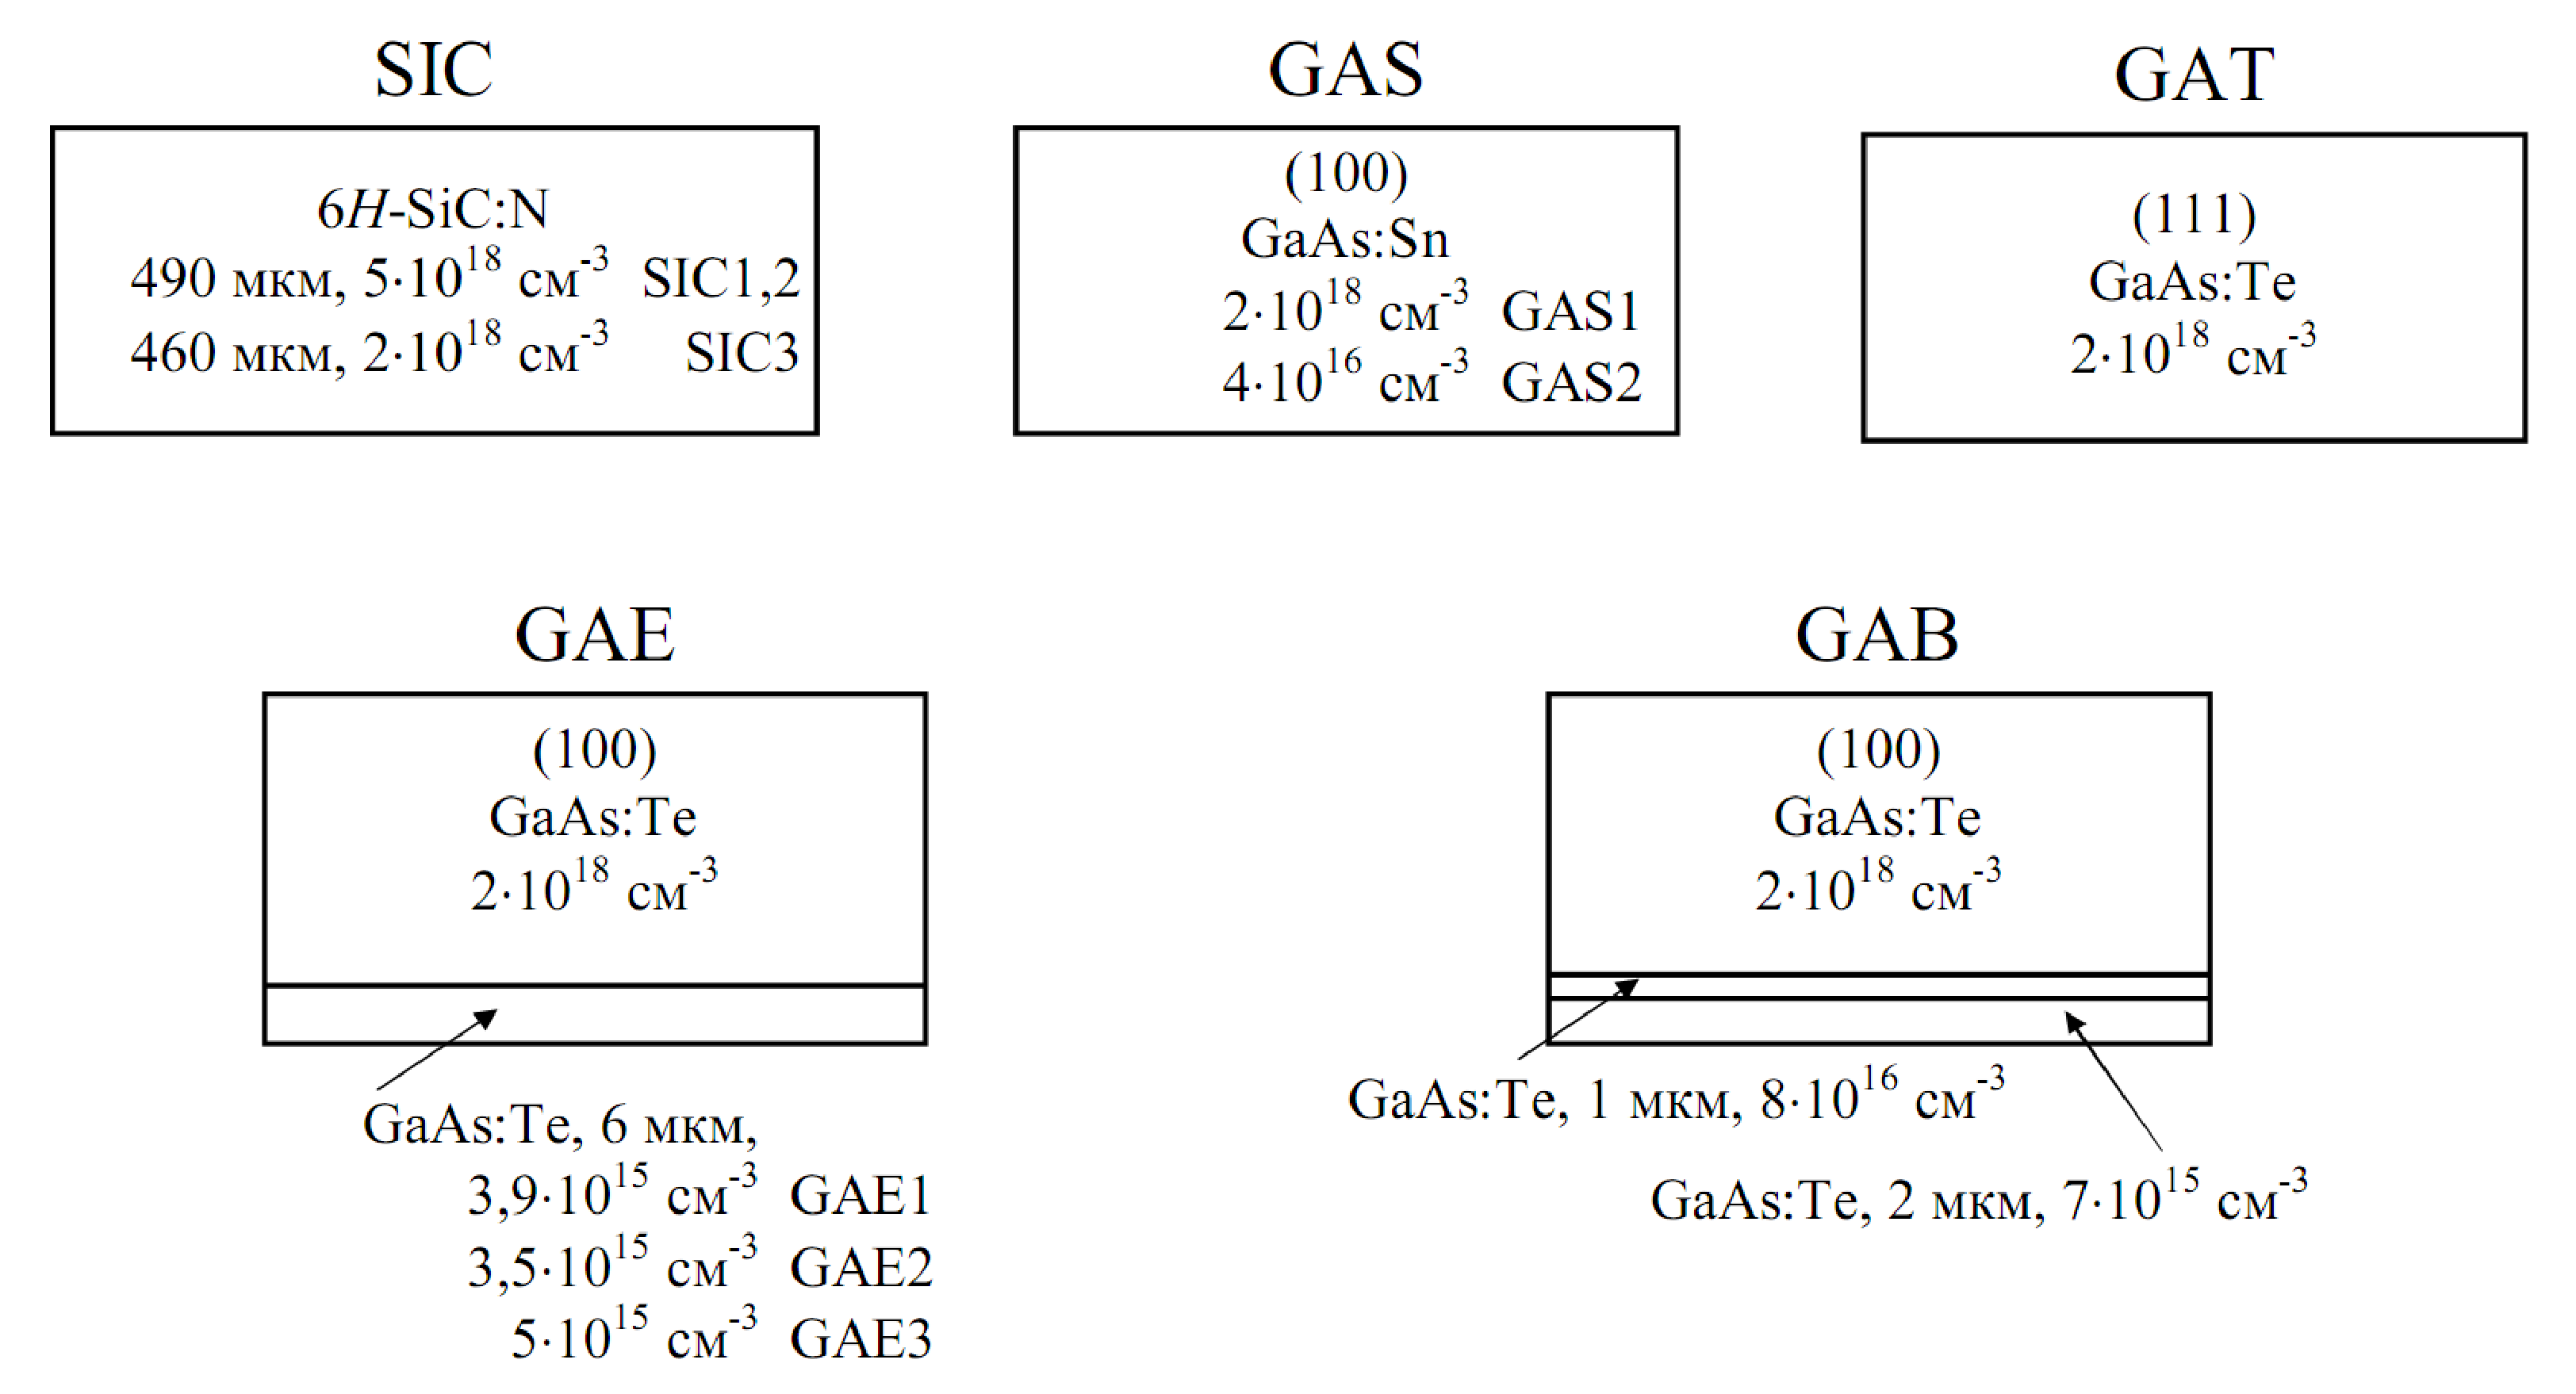
\includegraphics[width=0.95\textwidth]{figSamp_TAV}
\caption{\label{figSamp_TAV}
Структура зразків для вивчення глибоких рівнів.
}%
\end{figure}

МХО зразків проводилася у вільному просторі при кімнатній температурі в магнетроні на частоті 2,45 ГГц з питомою потужністю  $1,5$~Вт/см$^2$.
Опромінення епітаксійних структур здійснювалося з боку розташування епітаксійного шару.
Загальний час експозиції $t_\mathtt{MWT}$ змінювався в інтервалі $20\div60$~c для різних зразків.
З метою запобігання суттєвого нагріву зразків тривалість неперервного опромінення складала 5~с.

До та після МХО визначалися такі параметри глибоких центрів, як ефективний поперечний переріз захоплення електронів $\sigma_n$
та розташування енергетичного рівня центру відносно дна зони провідності $E_c-E_t$.
Для цього використовувався метод акустоелектричної релаксаційної спектроскопії \cite{Saiko1993,OstrovPAN,OlikhSSC}.
Схема методу зображена на Рис.~\ref{figTAV}.
Зразки розміщувалися на п'єзоелектричній пластині LiNbO$_3$, в якій імпульсно збуджувалися АХ.
Поширення УЗ в пластині супроводжується електричним полем, яке проникало в напівпровідник.
Внаслідок акусто--електронної взаємодії в напівпровіднику виникає постійна напруга, пов'язана з перерозподілом носіїв заряду,
захоплених пастками, розташованими в приповерхневому шарі --- так звана поперечна акустоелектрична напруга (ПАН).
Після закінчення УЗ імпульсу відбувається релаксація ПАН згідно з законом
\begin{equation}\label{eqVtav}
  V_\mathtt{TAV}(t)=V_{\mathtt{TAV},0}\exp(-t/\tau).
\end{equation}

\begin{figure}
\center
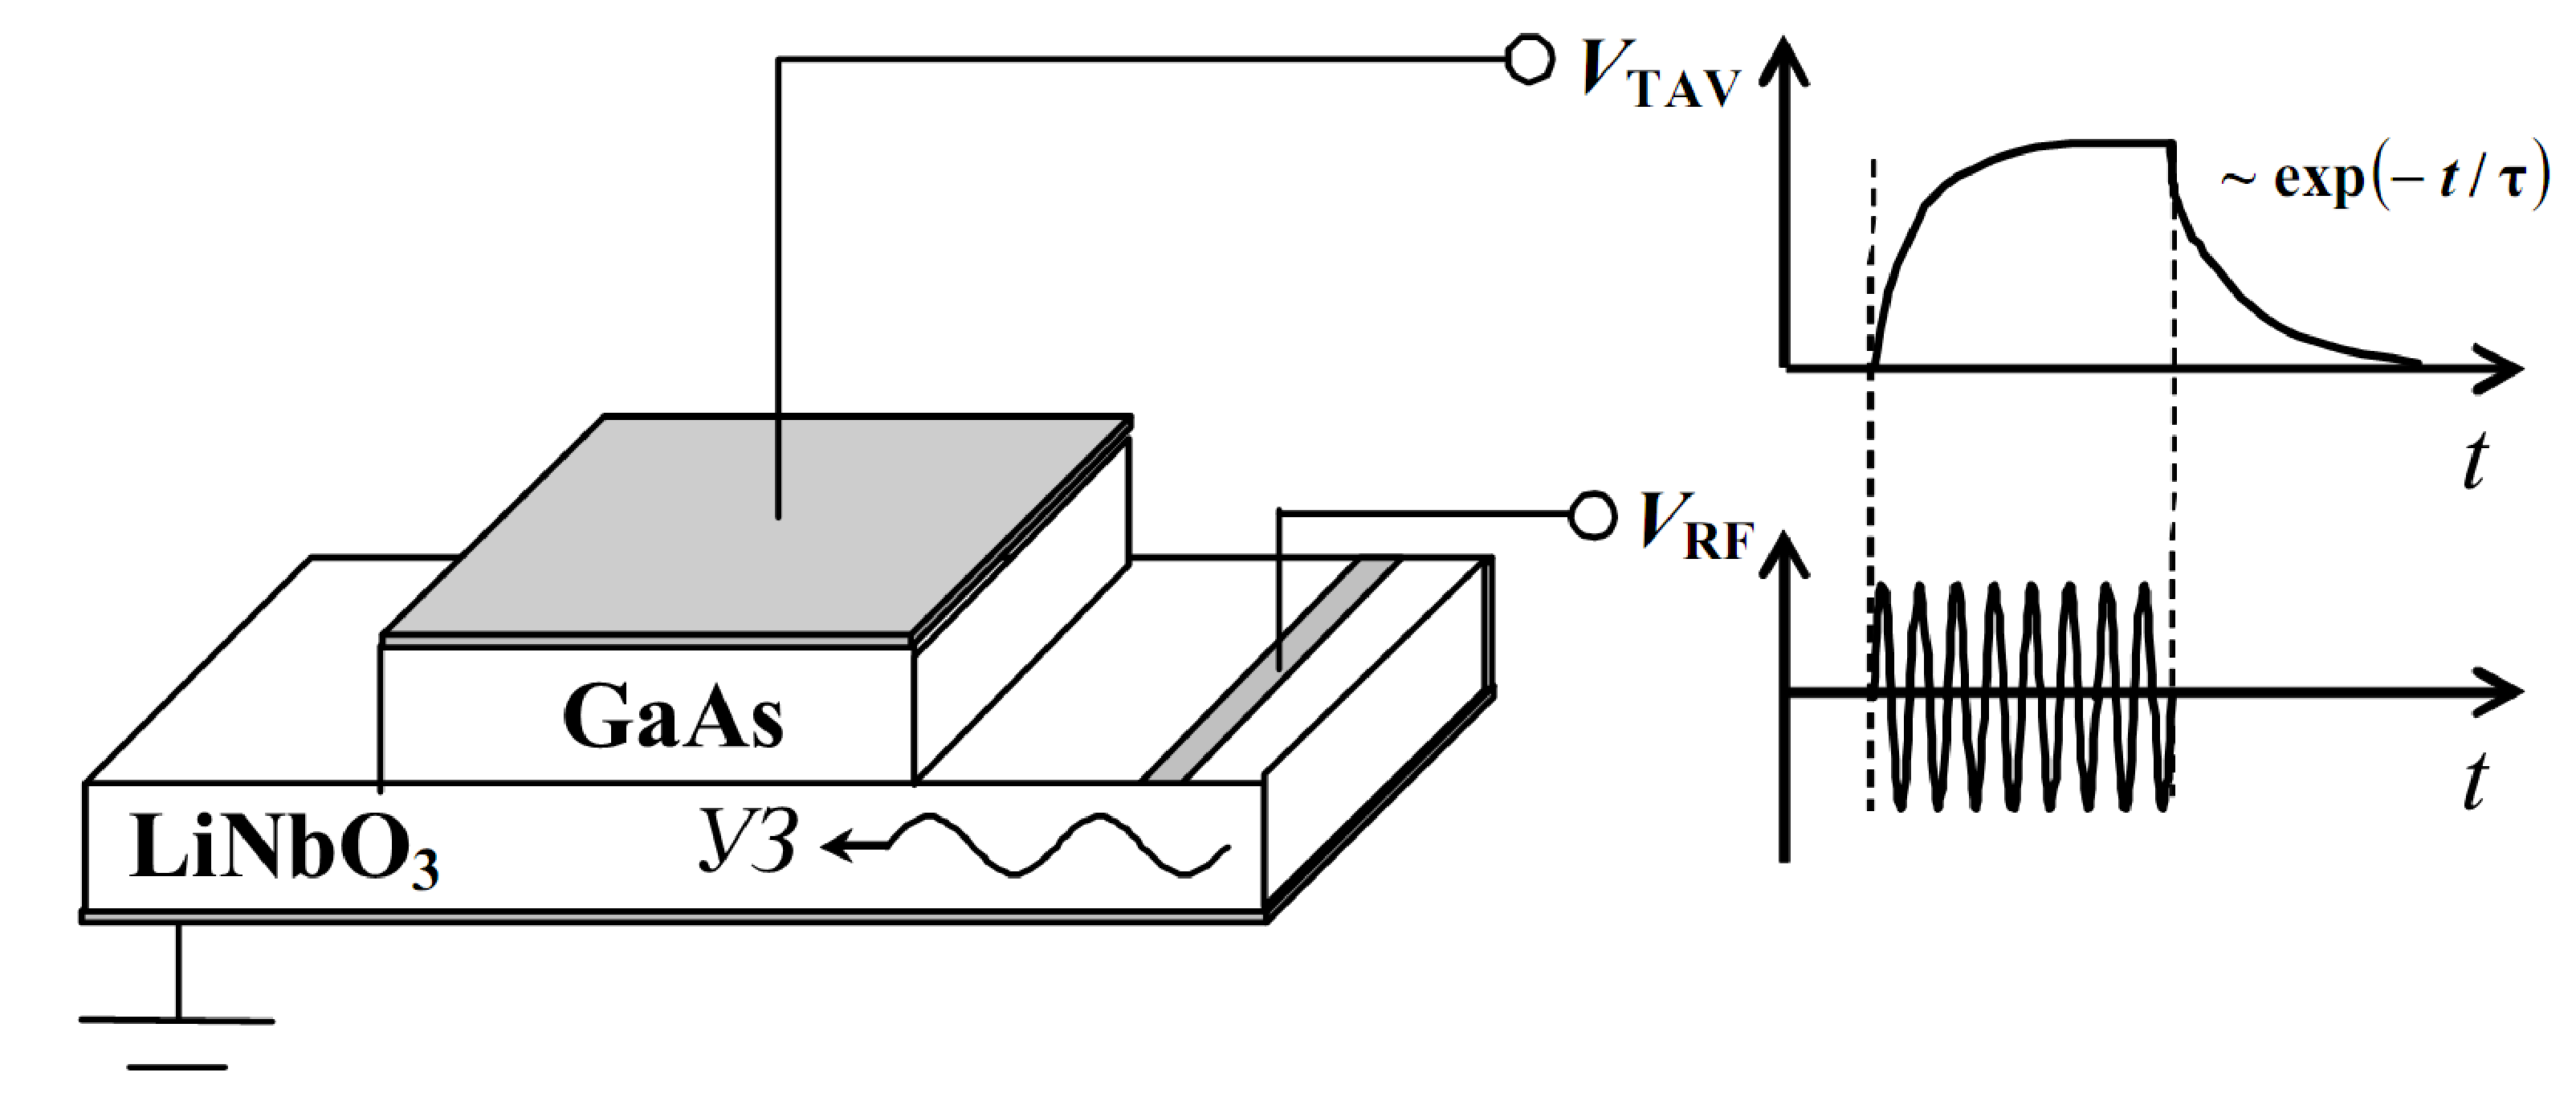
\includegraphics[width=0.8\textwidth]{figTAV}
\caption{\label{figTAV}
Схема вимірювання сигналу ПАН.
Схематично показано часові залежності радіоімпульсу $V_\mathtt{RF}$ для збудження УЗ в пластині п'єзоелектрика
та результуючого сигналу ПАН $V_\mathtt{TAV}$.
}%
\end{figure}

Проста експоненційна залежність (\ref{eqVtav}) спостерігається у випадку, коли у акустоелектронній взаємодії ефективно приймають участь глибокі центри лише одного типу.
Для електронного напівпровідника характерний час релаксації описується співвідношенням \cite{Saiko1993,Rzanov,OstrovPAN}
\begin{equation}\label{eqPANtau}
  \tau=\frac{1}{\sigma_n\,\upsilon_{\mathrm{th},n}\,N_c}\exp\left(\frac{E_c-E_t}{kT}\right).
\end{equation}
Експериментальні вимірювання релаксаційної ділянки ПАН при різних температурах та їх подальша апроксимація згідно з (\ref{eqVtav}) дозволяли отримати
залежність $\tau(T)$.
Величина $E_c-E_t$ визначалась за нахилом залежності $\tau$ від $(kT)^{-1}$ у напівлогарифмічному масштабі, після чого, з використанням формули (\ref{eqPANtau}),
був розрахований $\sigma_n$.
Виміри проводилися в інтервалі температур $(290\div350)$~К,
за виключенням зразків GAB, для який ПАН досягала достатньої для вимірювання величини лише після нагріву до температур вище 310~К.

Для монокристалічних зразків до та після МХО також були проведені визначення радіуса кривизни $R_\mathtt{cur}$ та
деформації $\xi_\mathtt{cur}$ приповерхневих кристалографічних площин.
Величина $\xi_\mathtt{cur}$ оцінювалася рентгенографічним методом по зміні кутового положення дифракційного максимуму при трансляції зразка \cite{Godwod},
кривизна вимірювалася на профілометрі DekTak 3030 Veeco Instruments.
$R_\mathtt{cur}$ та $\xi_\mathtt{cur}$ вимірювалися  з відносною похибкою, що не перевищувала 2~\%.
Для монокристалів арсеніду досліджувався також характер розподілу структурних дефектів по площі за допомогою методу
рентгенівської проекційної топографії за Борманом,
а розподіл густини дислокацій та мікронапруг визначався методом аналізу інтенсивності фріделівських пар відбиттів $hkl$ та $hk\overline{l}$ \cite{ThoricBook}.


\subsection{Вплив мікрохвильових обробок на параметри глибоких рівнів}

На Рис.~\ref{figTauTAV} наведено типові температурні залежності $\tau$ для зразків до та після МХО.
З наведених даних видно, що після дії НВЧ опромінення змінюється як нахил кривих (безпосередньо пов'язаний
з розташуванням рівня у забороненій зоні), так і абсолютна величина характерного часу релаксації ПАН.
Характер та величина впливу залежать як від часу експозиції, так і від ступеня легування та внутрішньої будови
досліджених структур.
Отримані результати узагальнені в Таблиці~\ref{tabMW}.
Видно, що в зразках карбіду кремнію зустрічається 2 глибокі рівні, позначені ESC1 та ESC2,
в зразках арсеніду галію --- шість (EGA1--EGA6).


\begin{figure}
\center
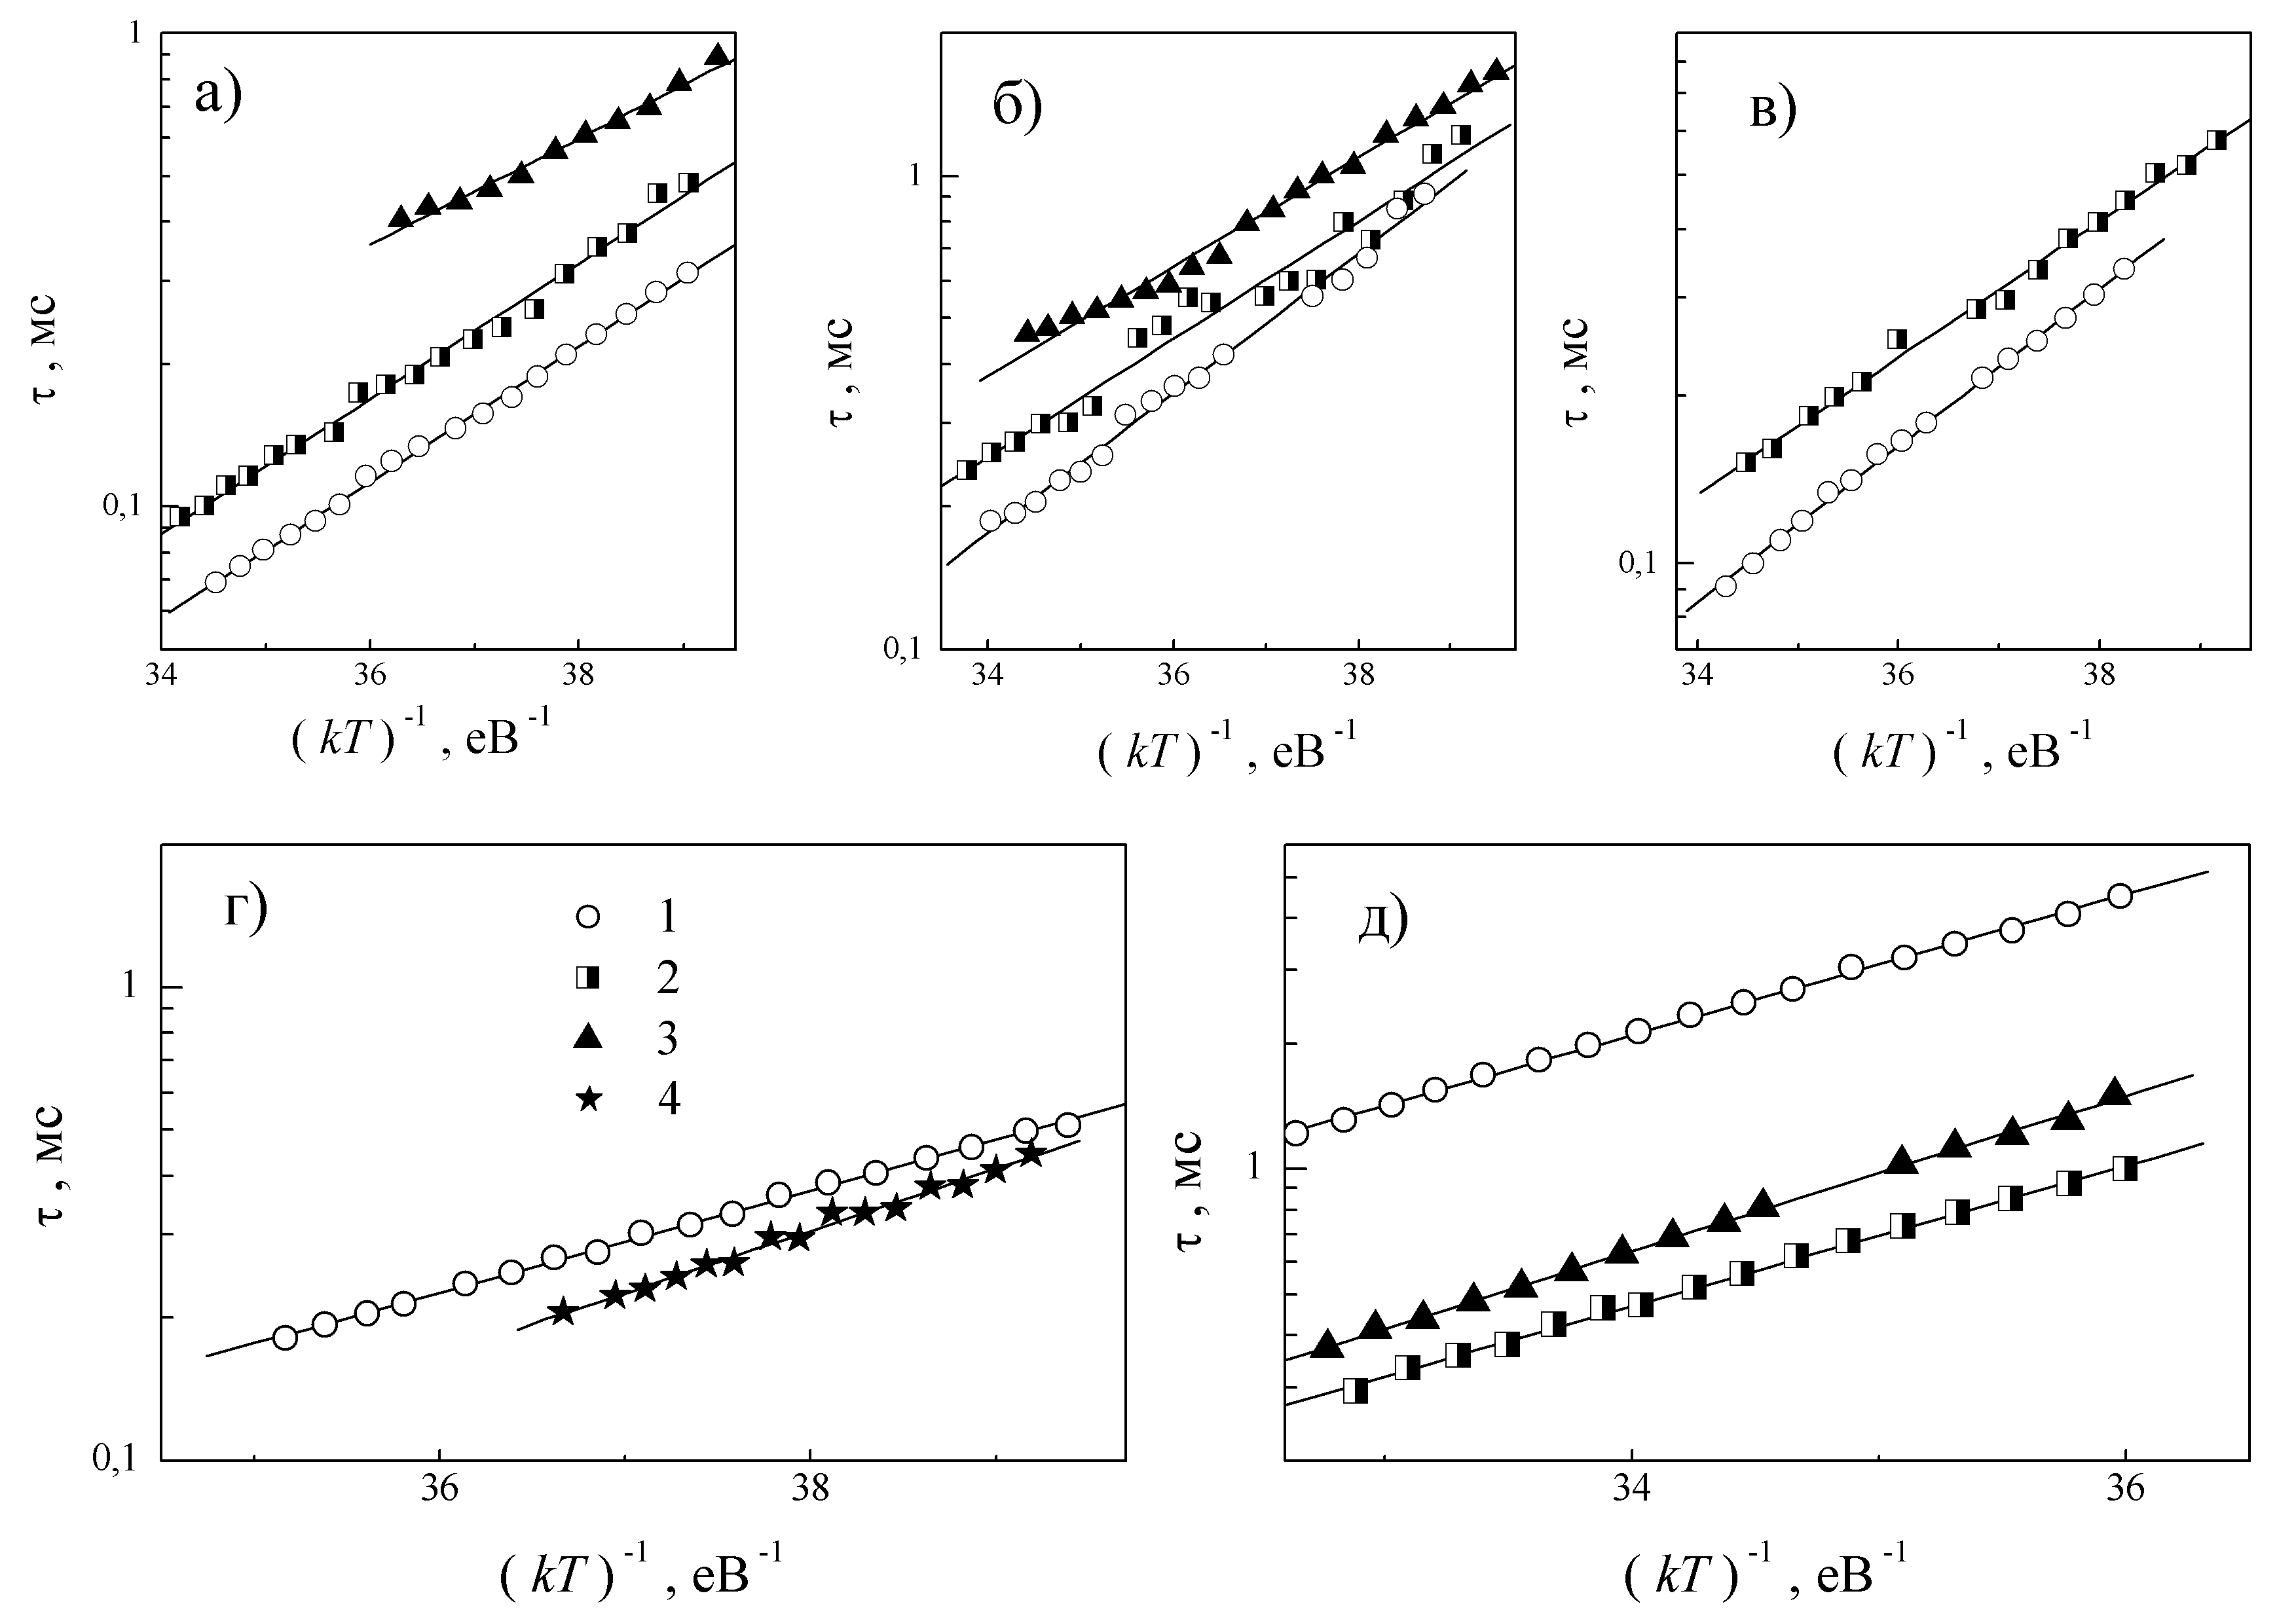
\includegraphics[width=0.99\textwidth]{figTauTAV}
\caption{\label{figTauTAV}
Залежності часу релаксації ПАН від оберненої температури для
зразків SIC2 (а), SIC3 (б), GAS2 (в), GAE2 (г) та GAB1 (д) до та після МХО.
$t_\mathtt{MWT}$, c: 0 (криві 1), 20 (2), 40 (3), 60 (4).
}%
\end{figure}

\begin{table}
\caption{\label{tabMW}Визначені параметри зразків $n$--GaAs та $n$--6$H$--SiC.
}
\center
\begin{tabular}{|c|c|c|c|c|c|c|}
\hline
%Зразок& $t_\mathtt{MWT}$, c & $(E_c-E_t)$, еВ &$\sigma_n$, см$^2$\textsuperscript{ a)}&$R_\mathtt{cur}$, м&$\xi_\mathtt{cur}$\\
Зразок& $t_\mathtt{MWT}$, c &Рівень &$(E_c-E_t)$, еВ &$\sigma_n$, см$^2$\textsuperscript{ a)}&$R_\mathtt{cur}$, м&$\xi_\mathtt{cur}$\\
\hhline{|=======|}
SIC1& 0 &ESC1& $0,33\pm0,01$ &$(7\pm4)\cdot10^{-18}$&$\infty$&0\\ \cline{2-7}
& 20 &ESC1& $0,33\pm0,01$ &$(5\pm3)\cdot10^{-19}$&170,2&$8,7\cdot10^{-7}$\\ \cline{2-7}
& 40 &ESC2& $0,26\pm0,01$ &$(2\pm1)\cdot10^{-19}$&\multicolumn{2}{c|}{\multirow{2}{*}{н/в}}\\ \cline{2-5}
& 80 & \multicolumn{3}{c|}{c/c}&\multicolumn{2}{c|}{}\\ \hline
SIC2& 0 &ESC1& $0,33\pm0,01$ &$(7\pm4)\cdot10^{-18}$&$>2000$&$<1,2\cdot10^{-7}$\\ \cline{2-7}
& 20 &ESC1& $0,33\pm0,01$ &$(5\pm3)\cdot10^{-19}$&171,9&$1,4\cdot10^{-6}$\\ \hline
SIC3& 0 &ESC1& $0,34\pm0,02$ &$(3\pm2)\cdot10^{-18}$&3,8&$6,1\cdot10^{-5}$\\ \cline{2-7}
& 20 &ESC2&$0,29\pm0,01$ &$(5\pm3)\cdot10^{-19}$&5,5&$4,2\cdot10^{-5}$\\ \cline{2-7}
& 40 &ESC2& $0,26\pm0,01$ &$(10\pm7)\cdot10^{-20}$&\multicolumn{2}{c|}{\multirow{2}{*}{н/в}}\\ \cline{2-5}
& 80 &ESC2& $0,23\pm0,01$ &$(6\pm4)\cdot10^{-20}$&\multicolumn{2}{c|}{}\\ \hline
GAS1& 0 &EGA1& $0,32\pm0,02$ &$(3\pm2)\cdot10^{-17}$&-53,8&$-2,8\cdot10^{-6}$\\ \cline{2-7}
& 20 &EGA1& $0,31\pm0,01$ &$(2\pm1)\cdot10^{-17}$&22,9&$6,5\cdot10^{-6}$\\ \cline{2-7}
& 40 & \multicolumn{3}{c|}{c/c}&\multicolumn{2}{c|}{н/в}\\ \hline
GAS2& 0 &EGA1& $0,32\pm0,01$ &$(4\pm2)\cdot10^{-17}$&17,2&$8,7\cdot10^{-6}$\\ \cline{2-7}
& 20 &EGA2& $0,28\pm0,01$ &$(5\pm2)\cdot10^{-18}$&14,7&$1,0\cdot10^{-5}$\\ \cline{2-7}
& 40 & \multicolumn{3}{c|}{c/c}&\multicolumn{2}{c|}{}\\ \cline{1-5}
GAT& 0 &EGA3& $0,49\pm0,02$ &$(5\pm3)\cdot10^{-14}$&\multicolumn{2}{c|}{}\\ \cline{2-5}
& 20 &EGA4& $0,40\pm0,02$ &$(2\pm1)\cdot10^{-15}$&\multicolumn{2}{c|}{}\\ \cline{1-5}
GAE1& 0 &EGA5& $0,24\pm0,01$ &$(2\pm1)\cdot10^{-18}$&\multicolumn{2}{c|}{}\\ \cline{2-5}
& 60 &EGA2& $0,29\pm0,01$ &$(10\pm6)\cdot10^{-18}$&\multicolumn{2}{c|}{}\\ \cline{1-5}
GAE2& 0 &EGA5& $0,25\pm0,01$ &$(2\pm1)\cdot10^{-18}$&\multicolumn{2}{c|}{}\\ \cline{2-5}
& 60 &EGA2& $0,30\pm0,01$ &$(2\pm1)\cdot10^{-17}$&\multicolumn{2}{c|}{}\\ \cline{1-5}
GAE3& 0 &EGA6& $0,43\pm0,01$ &$(8\pm5)\cdot10^{-17}$&\multicolumn{2}{c|}{н/в}\\ \cline{2-5}
& 60 &EGA6& $0,46\pm0,02$ &$(7\pm4)\cdot10^{-16}$&\multicolumn{2}{c|}{}\\ \cline{1-5}
GAB1& 0 &EGA4& $0,39\pm0,01$ &$(10\pm7)\cdot10^{-18}$&\multicolumn{2}{c|}{}\\ \cline{2-5}
& 20 &EGA4& $0,39\pm0,01$ &$(4\pm2)\cdot10^{-17}$&\multicolumn{2}{c|}{}\\ \cline{2-5}
& 40 &EGA6& $0,43\pm0,02$ &$(10\pm6)\cdot10^{-17}$&\multicolumn{2}{c|}{}\\ \cline{1-5}
GAB2& 0 &EGA4& $0,40\pm0,01$ &$(10\pm6)\cdot10^{-17}$&\multicolumn{2}{c|}{}\\ \cline{2-5}
& 20 &EGA4& $0,41\pm0,01$ &$(10\pm6)\cdot10^{-17}$&\multicolumn{2}{c|}{}\\ \cline{2-5}
& 40 &EGA6& $0,45\pm0,02$ &$(4\pm2)\cdot10^{-16}$&\multicolumn{2}{c|}{}\\  \hline
\multicolumn{6}{l}{\textsuperscript{ a)} \emph{при $T=300$~К для SIC, GA, GAE та при  $T=340$~К для GAB}}\\
\multicolumn{6}{l}{\emph{н/в --- вимірювання не проводилися; с/с --- слабкий сигнал ПАН}}\\
%\multicolumn{6}{l}{\emph{с/с --- величина ПАН недостатня для визначення параметрів пасток}}\\
\end{tabular}
\end{table}

Для наведених даних є характерною низка особливостей.
А саме.
\begin{enumerate}[label=\arabic*),leftmargin=0em,itemindent=1.5em]
\item Величина перерізу захоплення носіїв значно чутливіша до МХО, ніж енергетичне розташування рівнів.
Так, наприклад, виявлено зміни $\sigma_n$ на порядок величини, тоді як зміщення положення рівнів не перевищує 20\%;
крім того, модифікація перерізу захоплення спостерігається при менших часах експозиції: так, наприклад,
для GAB1 після 20~с НВЧ впливу значення $(E_c-E_t)$ практично не змінилося, тоді як $\sigma_n$ зросла приблизно в чотири рази.

\item В монокристалах ступінь індукованих МХО змін зростає при зменшенні концентрації вільних носіїв заряду (див. дані для зразків GAS1 та GAS2) та зростанні відносної деформації (зменшенні кривизни поверхні).

\item Після тривалої (для GaAs $t_\mathtt{MWT}\geq40$~с, для SiC $t_\mathtt{MWT}\geq80$~с) МХО монокристалічних
зразків спостерігається суттєве зменшення сигналу ПАН.
Це корелює з даними роботи \cite{Belyaev1998JTFr}, автори якої спостерігали зменшення концентрації центрів, що
мають енергетичні рівні у верхній половині забороненої зони внаслідок НВЧ відпалу.

\item Доза опромінення, необхідна для суттєвого впливу на параметри центрів в епітаксійних структурах, вища, ніж
для монокристалічних зразків.
Зокрема, про це свідчать дані Таблиці~\ref{tabMW} для зразків серій GA та GAB після опромінення протягом 20~с.
Зауважимо, що легування підкладки та епі--шару структур GAB співпадало за рівнем зі зразками GAS1 і GAT та GAS2, відповідно; окрім того, тип легуючої домішки  GAB та GAT також однаковий.
Отже виявлені відмінності не можуть бути пов'язані з провідністю, а визначаються саме топологією структур.

\item Характер змін у монокристалічних пластинах та епітаксійних структурах протилежний:
для SIC, GAS, GAT після МХО спостерігається зменшення $\sigma_n$ та $(E_c-E_t)$, тоді як в GAE та GAB обидва параметри зростають.
\end{enumerate}

Спираючись на літературні дані, розглянемо можливу природу центрів,
які виявлені у досліджених структурах.
При цьому необхідно врахувати, що літературні дані характеризуються наявністю розкиду значень основних параметрів
пасток, зокрема відмінності величини поперечного перерізу захоплення можуть досягати чотирьох порядків \cite{Pavlovic2000}.
Однією з можливих причин цього феномену може бути суттєва залежність швидкості термічної емісії носіїв від
напруженості електричного поля  \cite{Bulyarskii2000r,Makram,Shishiyanu},
яка викликана
а)~зменшення енергії іонізації внаслідок ефекту Пула--Френкеля чи, наприклад,
завдяки кулонівській взаємодії центрів \cite{Stellmacher};
б)~зміною величини $\sigma_n$ \cite{Shishiyanu,Bourgoin2001}.
Як правило, зміни $(E_c-E_t)$ складають декілька сотих еВ, тоді
зміни перерізу захоплення можуть досягати декількох порядків:
наприклад, згідно з даними роботи \cite{Bourgoin2001},  при кімнатній температурі $\sigma_n$ для центру EL2 в GaAs при напруженості $10^5$~В/см збільшується в 200 разів.
Як наслідок, при використанні різних методів дослідження дефектів отримані параметри одних і тих же центрів
можуть суттєво відрізнятися.
Наприклад, можна порівняти результати оглядових робіт, де зібрані дані по різноманітним пасткам в арсеніді галію отримані за допомогою методів нестаціонарної емнісної спектроскопії \cite{Bourgoin:GaAs} та
термостимульованих струмів \cite{Pavlovic2000}.
Наведені дані стосуються дефектів з близьким положенням рівнів і суттєво різними значеннями поперечного перерізу захоплення.
Узагальнюючи сказане, зауважимо, що при ідентифікації дефектів будемо орієнтуватися саме на енергетичне розташування
пасткових рівнів.


Положення рівня ESC1 ($E_c-(0,33\div0,34)$~еВ), який спостерігався у вихідних монокристалах карбіду кремнію
можна зіставити з розташуванням $S$--центру ($E_c-0,35)$~еВ, \cite{Lebed1999,Anikin1991:2,Anikin1991:3}),
$EK3$--центру ($E_c-0,34)$~еВ, \cite{Kuznets1997}) чи рівня $(-/+)$ центру $E_1$ ($E_c-0,34)$~еВ, \cite{Lebed1999}).
$S$--центр відповідає за безвипромінювальну рекомбінацію і відноситься до власних дефектів в 6$H$--SiC \cite{Lebed1999}).
Згідно з результатами робіт \cite{Anikin1991:2,Anikin1991:3} $S$--центр та $R$--центр ($E_c-1,27)$~еВ) пов'язані
з двома різними зарядовими станами одного й того ж дефекту, тоді як відповідно до даних роботи \cite{Lebedev2000}
$R$--центр є дивакансією V$_\text{Si}+$V$_\text{C}$.
З рівнем $E_1$, який є центром з від'ємною кореляційною енергією,
пов'язують комплекс кремнієвих вакансій  \cite{Lebedev2001}.
Після МХО розташування рівня, що відповідає за появу ПАН в SIC, змінюється до $E_c-(0,26\div0,29)$~еВ (рівень ESC2).
В цьому випадку також немає повної однозначності:
близьке положення має рівень донорний рівень $(0/+)$ центру $E_1$ ($E_c-(0,27\div0,28)$~еВ, \cite{Hemmingsson})
та центр $X_1$ ($E_c-0,3)$~еВ, \cite{Lebedev2001}).
Автори останньої роботи доповідають про суттєву залежність концентрації $X_1$ від структурної
досконалості кристалу та підкреслюють не ідентичність цього центру  та  дослідженого раніше $E_1$.

Для для центрів в  арсеніді галію представлені значно ширше.
Узагальнені дані для кожного з виявлених рівнів узагальнено в Таблицях~\ref{tabEGA1}--~\ref{tabEGA6}.
Наведені дані показують, що виявлені центри пов'язані з власними дефектами, переважно вакансійного типу.

\begin{table}
\caption{\label{tabEGA1}Літературні дані для рівнів, близьких за розташуванням до EGA1
($E_c-E_t=(0,31\div0,32)$~еВ, $\sigma_n\approx3\cdot10^{-17}$~см$^2$, виявлений в зразках GAS1 та GAS2).
}
\center
\begin{tabular}{|c|c|c|c|c|c|}
\hline
$(E_c-E_t)$, еВ &$\sigma_n$, см$^2$&конфігурація&метод&епі--структура&посилання\\ \hline
0,33&&комплекс з V$_\text{As}$&DLTS&ні&\cite{EL6:Richter}\\ \hline
0,33&&&DLTS&ні&\cite{Neild1991}\\ \hline
$0,31\div0,33$&&V$_\text{As}$&&&\cite{EL6:Schultz}\\ \hline
0,33&$1\cdot10^{-17}$&&TSC&ні&\cite{Pavlovic2000}\\ \hline
0,323&$1\cdot10^{-14}$&&DLTS&так&\cite{Yousefi1995}\\ \hline
0,334&$2\cdot10^{-15}$&&DLTS&так&\cite{Yousefi1995}\\ \hline
0,35&&комплекс з V$_\text{As}$&PA&ні&\cite{EL6:Kuisma}\\ \hline
$0,315\div0,325$&$3\cdot10^{-17}$&&TSC&ні&\cite{Pavlovic:GaAs}\\ \hline
0,33&&&TSC&ні&\cite{Tomozane:GaAs}\\ \hline
$0,30\div0,33$&&&DLTS&ні&\cite{Lang:GaAs}\\ \hline
\multicolumn{6}{l}{ \emph{DLTS --- метод нестаціонарної спектроскопії ГР}}\\
\multicolumn{6}{l}{ \emph{TSC --- метод термостимульованих струмів}}\\
\multicolumn{6}{l}{ \emph{PA --- позитрон--анігіляційна спектроскопія}}\\
\end{tabular}
\end{table}


\begin{table}
\caption{\label{tabEGA2}Літературні дані для рівнів, близьких за розташуванням до EGA2
($E_c-E_t=(0,31\div0,32)$~еВ, $\sigma_n\approx5\cdot10^{-18}$~см$^2$ (монокристали),
$1\cdot10^{-17}$~см$^2$ (епі-структури), виявлений в зразках GAS2, GAE1 та GAE2 після опромінення).
}
\center
\begin{tabular}{|c|c|c|c|c|c|}
\hline
$(E_c-E_t)$, еВ &$\sigma_n$, см$^2$&конфігурація&метод&епі--структура&посилання\\ \hline
0,28&$5\cdot10^{-18}$&V$_\text{As}$As$_i$&TSC&ні&\cite{Pavlovic2000}\\ \hline
0,26&$3,5\cdot10^{-15}$&&DLTS&так&\cite{Yousefi1995}\\ \hline
$0,277$&$5\cdot10^{-17}$&&TSC&ні&\cite{Pavlovic:GaAs}\\ \hline
$0,284$&$1\cdot10^{-17}$&&TSC&ні&\cite{Pavlovic:GaAs}\\ \hline
0,28&&власний&TP&ні&\cite{Abele:GaAs}\\ \hline
0,28&$8\cdot10^{-15}$&&DLTS&так&\cite{Mircea1975}\\ \hline
0,30&&комплекс з Те&DLTS&ні&\cite{KolFTP1994r}\\ \hline
0,30&$6\cdot10^{-15}$&V$_\text{As}$As$_i$&DLTS&ні&\cite{Pons}\\ \hline
\multicolumn{6}{l}{\emph{TP --- релаксація фотопровідності}}\\
\end{tabular}
\end{table}



\begin{table}
\caption{\label{tabEGA3}Літературні дані для рівнів, близьких за розташуванням до EGA3
($E_c-E_t=0,49$~еВ, $\sigma_n\approx5\cdot10^{-14}$~см$^2$ виявлений в зразку GAТ).
}
\center
\begin{tabular}{|c|c|c|c|c|c|}
\hline
$(E_c-E_t)$, еВ &$\sigma_n$, см$^2$&конфігурація&метод&епі--структура&посилання\\ \hline
0,50&&Sb$_\text{Ga}$&DLTS&ні&\cite{Samoilov1994}\\ \hline
0,48&$4\cdot10^{-16}$&As$_\text{Ga}^{++}$&TSC&ні&\cite{Pavlovic2000}\\ \hline
$0,485$&$2\cdot10^{-16}$&&TSC&ні&\cite{Pavlovic:GaAs}\\ \hline
$0,48$&&домішка&TP&ні&\cite{Abele:GaAs}\\ \hline
0,51&$1\cdot10^{-12}$&&DLTS&ні&\cite{Martin1977}\\ \hline
0,48&$3\cdot10^{-13}$&&DLTS&ні&\cite{Lang:GaAs}\\ \hline
0,50&$1\cdot10^{-15}$&V$_\text{As}$, V$_\text{Ga}$Ga$_i$V$_\text{As}$ &DLTS&ні&\cite{Pons}\\ \hline
\end{tabular}
\end{table}

\begin{table}
\caption{\label{tabEGA4}Літературні дані для рівнів, близьких за розташуванням до EGA4
($E_c-E_t=(0,39\div0,41)$~еВ, $\sigma_n\approx2\cdot10^{-15}$~см$^2$ (монокристали),
$(1\div10)\cdot10^{-17}$~см$^2$ (епі-структури), виявлений в зразках GAТ та GAB).
}
\center
\begin{tabular}{|c|c|c|c|c|c|}
\hline
$(E_c-E_t)$, еВ &$\sigma_n$, см$^2$&конфігурація&метод&епі--структура&посилання\\ \hline
0,42&&&DLTS&ні&\cite{Neild1991}\\ \hline
0,41&&V$_\text{Ga}$V$_\text{As}$&DLTS&ні&\cite{Samoilov1994}\\ \hline
$0,39$&&V$_\text{Ga}$Ga$_\text{As}$&TSC&ні&\cite{FANG1990}\\ \hline
$0,41$&$2\cdot10^{-13}$&&DLTS&так&\cite{Bourgoin:GaAs}\\ \hline
0,40&&&SCRC&так&\cite{ASHBY:GaAs}\\ \hline
0,37&$2\cdot10^{-14}$&&DLTS&так&\cite{Fang:EL6}\\ \hline
0,40&&V$_\text{Ga}$Ga$_\text{As}$&DLTS&ні&\cite{Vaitkus}\\ \hline
0,387&$2\cdot10^{-14}$&&DLTS&так&\cite{Yousefi1995}\\ \hline
\multicolumn{6}{l}{\emph{SCRC --- температурна залежність струму ОПЗ}}\\
\end{tabular}
\end{table}



\begin{table}
\caption{\label{tabEGA5}Літературні дані для рівнів, близьких за розташуванням до EGA5
($E_c-E_t=(0,24\div0,25)$~еВ, $\sigma_n\approx2\cdot10^{-18}$~см$^2$, виявлений в зразках GAE1 та GAE2 до опромінення).
}
\center
\begin{tabular}{|c|c|c|c|c|c|}
\hline
$(E_c-E_t)$, еВ &$\sigma_n$, см$^2$&конфігурація&метод&епі--структура&посилання\\ \hline
0,23&&&DLTS&ні&\cite{Neild1991}\\ \hline
0,23&$2\cdot10^{-17}$&&TSC&ні&\cite{Pavlovic2000}\\ \hline
$0,22\div0,25$&$8\cdot10^{-19}$&&TSC&ні&\cite{Lin:GaAs}\\ \hline
$0,26$&&комплекс з V$_\text{Ga}$&TSC&ні&\cite{FANG1990}\\ \hline
0,24&&&TSC&ні&\cite{Tomozane:GaAs}\\ \hline
0,23&&власний&TP&ні&\cite{Abele:GaAs}\\ \hline
0,23&&V$_\text{Ga}$V$_\text{As}$&DLTS&ні&\cite{Morrow:EL17}\\ \hline
0,23&$1\cdot10^{-14}$&V$_\text{Ga}$V$_\text{As}$&DLTS&ні&\cite{Bourgoin:GaAs}\\ \hline
0,23&$7\cdot10^{-15}$&&DLTS&так&\cite{Mircea1975}\\ \hline
0,22&$2\cdot10^{-15}$&&DLTS&ні&\cite{Fang:EL6}\\ \hline
0,258&$4\cdot10^{-16}$&&DLTS&так&\cite{Yousefi1995}\\ \hline
\end{tabular}
\end{table}



\begin{table}
\caption{\label{tabEGA6}Літературні дані для рівнів, близьких за розташуванням до EGA6
($E_c-E_t=(0,43\div0,46)0,43$~еВ, $\sigma_n\approx8\cdot10^{-17}$~см$^2$ (GAE3 до опромінення)
$\sigma_n\approx5\cdot10^{-16}$~см$^2$ (GAE3, GAB після опромінення)).
}
\center
\begin{tabular}{|c|c|c|c|c|c|}
\hline
$(E_c-E_t)$, еВ &$\sigma_n$, см$^2$&конфігурація&метод&епі--структура&посилання\\ \hline
0,44&$1\cdot10^{-14}$&V$_\text{As}$As$_i$, V$_\text{As}$&TSC&ні&\cite{Pavlovic2000}\\ \hline
0,44&$9\cdot10^{-15}$&&TSC&ні&\cite{Pavlovic:GaAs}\\ \hline
$0,43$&$7\cdot10^{-16}$&власний&DLTS&так&\cite{Lefevre1977,Bourgoin:GaAs}\\ \hline
$0,44$&$2\cdot10^{-15}$&комплекс з V$_\text{As}$&DLTS&так&\cite{KolFTP1989r}\\ \hline
\end{tabular}
\end{table}


Можна виділити декілька причин зміни параметрів пасток.
А саме.
\begin{enumerate}[label=\arabic*),leftmargin=0em,itemindent=1.5em]
\item Перебудова дефектного комплексу внаслідок його розпаду, долучення додаткової компоненти, зміни відстані між складовими тощо.
\item Зміна зарядового стану дефекту.
\item Зміна оточення пастки, що призводить, наприклад, до модифікації напруженості електричного поля в околі дефекту.
\item Зміна концентрації дефектів даного типу: наприклад, в роботі \cite{Stellmacher} показано, що
зміна енергії іонізації пропорційна кубічному кореню з кількості дефектів в одиниці об'єму.
\end{enumerate}



При аналізі причин виявлених змін необхідно взяти до уваги можливі механізми впливу
мікрохвильового випромінювання на кристали.
Звичайно, в першу чергу варто врахувати ефекти збільшення температури.
Так, вважається, що  структурна модифікація внаслідок МХО пов'язана, переважно,
зі зміною зарядового стану дефектів та виникненням полів пружних напруг, обумовлених миттєвим розігрівом дефектних регіонів.
Проте, як відомо, для провідних твердих середовищ ці процеси підсилюються при зростанні концентрації вільних носіїв заряду \cite{MW:Rev}, тоді як в нашому випадку при зростанні $n$ виявлені ефекти послаблюються (див. дані для GAS1 та GAS2).
Крім того, використаний режим опромінення не передбачав довготривалого неперевного впливу НВЧ коливань, що також зменшувало загальний розігрів структур.
З іншого боку, багаточисленні дослідження показали, що виявлені ефекти не можуть бути пояснені лише з використанням механізмів швидкого термічного відпалу, а отже необхідно розглядати атермічні фактори.
В літературі останнім часом все більша увага приділяється нетепловим механізмам впливу МХО (див., наприклад, роботу \cite{MW:Si2018} та посилання в ній), які можуть бути причиною генерацію дислокацій та зменшення розмірів скупчень точкових дефектів в напівпровідникових пластинах \cite{Konakova2007JTF} чи навіть процесів рекристалізації \cite{MW:Si2018}.
В роботі \cite{Konakova2007JTF} проведено аналіз можливих атермічних процесів, які можуть викликати зміни структурних характеристик в бінарних напівпровідникових сполуках.
Зокрема розглянуто процеси коливання дислокацій під дією механічних напруг та електричного поля (останнє характерне для заряджених лінійних дефектів);
вказано, що суттєво впливати на поведінку дислокаційниних сегментів можуть декоруючі домішки:
з одного боку їх наявність знижує резонансну частоту коливань та забезпечує наявність електричного заряду,
а з іншого при великих амплітудах коливань вони можуть відриватися від дислокаційних ліній, що викликає появу додаткових хімічних дефектів.
В свою чергу, точкові дефекти можуть здійснювати НВЧ--коливання та дифундувати внаслідок МХО.



Виявлені зміни параметрів глибоких центрів, на нашу думку, пов'язані зі згаданою вище структурно--домішковою перебудовою приповерхневих областей напівпровідника внаслідок МХО.
Як показують результати рентгенографічних досліджень, НВЧ опромінення викликає збільшення опуклості монокристалічних зразків, що свідчить про накопичення в приповерхневому шарі дефектів міжвузольного типу,
зокрема внаслідок зародження окремих дислокацій  \cite{Boltovets,Konakova2012FTP}.
Подібне накопичення дефектів в поверхневій області матеріалу внаслідок дії НВЧ опромінення описується й іншими авторами \cite{Boltovets,Belyaev1998JTFr,Konakova2015}.
Певним виключенням є лише зразок SIC3, проте в цьому випадку і до опромінення спостерігався достатньо високий рівень
деформації приповерхневого шару.
Відомо \cite{Bacherikov2003r,Pashkov1994r,Boltovets,Kr1996,Milenin1994,BelyaevIntac}, що в такому напруженому стані МХО викликає перероздоділ пружних деформацій, який супроводжується їх певним зменшенням --- саме це і спостерігалося для SIC3.
Дані профілометрії корелюють з результатами рентгенівських вимірювань.
Структурні дослідження показали, що розподіл густини дислокацій по площі у вихідних пластинах GaAs має W--подібний характер;
густина дислокацій по діаметру пластини змінювалася від $2\cdot10^{4}$~см$^{-2}$ до $2\cdot10^{5}$~см$^{-2}$.
Така неоднорідність розподілу густини дислокацій вказує на значний рівень пружних деформацій в зразках.


На нашу думку, центри ESC1 та ESC2 є комплексами кремнієвих вакансій, EGA1 зв'язаний з V$_\text{As}$, а EGA3 --- з V$_\text{As}$ або комплексом V$_\text{Ga}$Ga$_i$V$_\text{As}$.
Стимульвана МХО дифузія точкових дефектів викликає модифікацію пасток.
Так, в карбіді кремнію центр ESC1 перетворюється на ESC2 внаслідок впливу близькорозташованого міжвузольного атому, подальша зміна параметрів якого (зразок SIC3) викликана підсиленням електричного поля протяжних дефектів.
В зразках GAS2 при $t_\mathtt{MWT}=20$~с внаслідок збільшення кількості міжвузольних атомів в приповерхневому шарі
відбувається перетворення V$_\text{As}$ на комплекс V$_\text{As}$As$_i$, з яким і пов'язаний центр EGA2.
В GAS1 цей процес утруднений внаслідок більшої концентрації носіїв заряду:
відомо \cite{ZOHM2000}, що з підвищенням опору зростає глибина проникнення НВЧ хвиль, а отже і об'єм, звідки відбувається гетерування дефектів у приповерхневому шарі.
Крім того, причиною слабкого (порівняно з GAS2) впливу МХО на параметри пасток в GAS1 є відсутність стискуючих напруг,
наявність яких, як показують дані для монокристалів карбіду кремнію, інтенсифікують стимульоване МХО комплексоутворення вакансій і міжвузольних атомів.
У зразку GAT, який також характеризуються високою концентрацією вільних електронів,
перетворення EGA3 на EGA4 (комплекс V$_\text{Ga}$Ga$_\text{As}$) відбувається згідно з реакцією, розглянутою в \cite{FANG1990}:
\begin{equation*}
  \text{V}_\text{Ga}\;\text{Ga}_{\,i}\;\text{V}_\text{As}\rightarrow \text{Ga}_\text{Ga}\;\text{V}_\text{As}
  \rightarrow \text{Ga}_\text{As}\;\text{V}_\text{Ga}
\end{equation*}
Накопичення великої кількості міжвузольних атомів в приповерхневому шарі при високих дозах опромінення ($t_\mathtt{MWT}\approx40$~с для арсеніду галію і $t_\mathtt{MWT}\geq80$~с для карбіду кремнію) викликає повну анігіляцію вакансій (або їх перетворення на антиструктурні дефекти, рівні яких в кристалах з електронною провідністю заповнені) і відповідне зникнення сигналу ПАН --- див. дані для зразків GAS1, GAS2, SIC1.


Вважається \cite{Saiko1993,OlikhSSC,OstrovPAN}, що в епітаксійних структурах поява ПАН, викликаної накопиченням зарядів на пастках, переважно пов'язана з дефектами, розташованими на границі розділу між епітаксійним шаром та підкладкою,
тобто на внутрішніх поверхнях.
Саме відмінність у просторовому розташуванні і є причиною, на нашу думку, різниці дозової залежності змін параметрів епітаксійних та монокристалічних зразків.

В роботах \cite{Boltovets,Konakova2012FTP} в епітаксійних структурах $n-n^+$--GaAs та $n-n^+-n^{++}$--GaAs спостерігалося індуковане МХО збільшення радіуса кривизни контактних систем внаслідок зародження окремих дислокацій та їх поширення вздовж площин ковзання вглиб структур.
Як наслідок, в приповерхневих регіонах відбуваються зміни напруженостей як електричного, так і механічного полів,
що і викликає перебудову дефектів, а отже і зміну розташування відповідних їм глибоких рівнів.

Як видно з даних Таблиць~\ref{tabEGA5} та \ref{tabEGA6}, рівні EGA5 та EGA6 зв'язані з комплексами V$_\text{Ga}$V$_\text{As}$ та V$_\text{As}$As$_i$, відповідно.
Такі пастки, як і EGA2 та EGA4, зустрічалися в епітаксійних структурах і раніше \cite{Yousefi1995,Mircea1975,Bourgoin:GaAs,ASHBY:GaAs,Fang:EL6,Lefevre1977,KolFTP1989r}.
Виявлені НВЧ-стимульовані перетворення пов'язані зі зростанням кількості міжвузольних атомів і описуються
реакціями на кшталт
\begin{equation*}
  \text{V}_\text{Ga}\;\text{V}_\text{As}+\text{Ga}_{\,i}+\text{As}_{\,i} \rightarrow \text{V}_\text{As}\;\text{As}_{\,i}
\end{equation*}
для GAE1 та GAE2 і
\begin{equation*}
  \text{V}_\text{Ga}\;\text{Ga}_\text{As}+\text{As}_{\,i} \rightarrow
  \text{Ga}_\text{Ga}\;\text{V}_\text{As}+\text{As}_{\,i} \rightarrow
  \text{V}_\text{As}\;\text{As}_{\,i}
\end{equation*}
для GAB1 та GAB2.
Збільшення енергії активації EGA6 в зразку GAE3 викликане, на нашу думку, зменшенням концентрації міжвузольно--вакансійних комплексів внаслідок зміни їх кулонівської взаємодії.
Зростання перерізу захоплення електронів пасток EGA4 в GAB1 при $t_\mathtt{MWT}=20$~c та EGA6 в GAE3 може бути пов'язане зі зростям напруженості електричного поля, пов'язаного з дислокаціями.


%СВЧ   Au–TiBx–Ge−Au–n––n+–n++-GaAs(InP)
%увеличением плотности дислокаций в
%приконтактной области полупроводника, обусловленной
%релаксацией внутренних механических напряжений в
%омическом контакте, что подтверждается увеличением
%радиуса кривизны контактных систем
%\cite{Konakova2012FTP}

%\cite{KorshunovBook,Kozlovs,Zaveryukhin2002:2,OlikhFTT,Boltovets,Bacherikov2003r,Belyaev1998JTFr,Saiko1993,OlikhSSC,
%Rzanov,Shishiyanu,Vaitkus,Samoilov1994,ZOHM2000}
%
%FCOM
%\cite{Rjanov1981,paton1993,Vinnik1989,ZOHM2000,BHUNIA1998,Bacherikov2003r,Pashkov1994r,Boltovets,Kr1996,Milenin1994,
%BelyaevIntac,ASHKINADZE1996,ProcSPIE,Venger1999,Godwod,ThoricBook,BergBook,Lebed1999,Anikin1991:2,
%Anikin1991:3,Lebedev2001}
%
%
%GaAs
%\cite{Neild1991}
%
%анігіляція позитронів
%EL6
%0.35 arsenic-vacancy-related defect complex \cite{EL6:Kuisma}
%
%TSC:
%рівні 0,34 , 4е-17;
%0.27-0.28, (1-5)е-17;
%0,315-0,325, 1е-17
%0,44 9е-15
%0,485 2е-16\cite{Pavlovic:GaAs}
%
%TSC:
%0.22-0.25, 8e-19;
%0.28
%0.35\cite{Lin:GaAs}
%
%TSC:
%0,39
%0,26
%0,21
%див. листок з реакціями \cite{FANG1990}
%
%TSC:
%0,22; 0,24; 0,33 - електронні пастки
%0,35, 0,39, 0,43 0,50 діркові \cite{Tomozane:GaAs}
%
%Great discrepancies in reported main trap parameters are
%obvious; up to four orders of magnitude for sn , for example,
%набор по TSC\cite{Pavlovic2000}
%
%
%Transient photoconductivity
%0.23 (називають EL8)
%0.28 (EL6)
%0.48
%власні дефекти \cite{Abele:GaAs}
%----------
%
%0.23 дивакансія (різних атомів) \cite{Morrow:EL17}
%
%0.23, 3e-14 дивакансія;
%вакансія мишьяку -  міжвузольний мишяк 0,30 а також 0,35, 2e-18
%0.42, 2e-13 EL5
%в газофазной епитаксии
%0.27, 8e-15 EL8
%0.225, 7e-15 EL9
%0.43, 7e-16 EI1
%MBE
%0.30, 1.7e-14 EB7  \cite{Bourgoin:GaAs} -- стаття називається власні дефекти
%
%0.40 газофазна епі--структура,
%температурна залежність струму ОПЗ \cite{ASHBY:GaAs}
%
%0,23; 0,28; 0,42 в газофазной епитаксии (попередня стаття сюди посилається і на дві наступні) \cite{Mircea1975}
%The  deep  level  (0.43 eV) observed in GaAs near the interface probably is caused
%by interdiffusion  of  an impurity from  the substrate into the  epilayer  during  the  growth  of the  layer. \cite{Lefevre1977}
%Trap M3  (0.30-0.33)  which  are dominant  in the As-rich samples
%0.48 3e-13
%DLTS \cite{Lang:GaAs}
%
%ще одна оглядова стаття, де є посилання на попередні три.. є ще рівень 0,51 \cite{Martin1977} в епі- за різною технологією можуть бути різні рівні
%
%EL6 0.35 1e-13 -- подвійна вкансія
%EL5 0.37 2e-14 (говорять, що в літературі 0,40+-0,02)
%обидва рівні спостерігаються в газофазновирощених шарах
%EL9 0.22 2e-15
%DLTS
%\cite{Fang:EL6}
%
%
%0.30, метастабильний (обумовлена контрольованою зарядовим станом внутрішньою перебудовою комплексу),
%комплекс, що містить атоми легуючої (Те) або залишкової домішки \cite{KolFTP1994r}
%
%0.44 1.5e-15 подложка n+-GaAs:Te,
%рівень спостерігається і в газофазних епі-структурах (тут -- хлоридним)
%EL5, зв'язаний з вакансією мишьяка \cite{KolFTP1989r}
%
%0.387; 0.334; 0.323; 0.258 на інтерфейсі епітаксійних?
%DLTS
%\cite{Yousefi1995}
%
%EL6, 0.33, комплекс з вакансією As \cite{EL6:Richter}
%EL6 - просто вакансія As \cite{EL6:Schultz}
%
%радіаційний 0,3 6е-15, щось зв'язане з парою вакансія миш'яку -- миш'як міжвузольний
%взагалі стверджується, що таких пар 4 утворюється при опромінення... відрізняються відстанню (впливом миш'як міжвузольний на вакансія миш'яку )
%0.5 1.4e-15
%DLTS
%\cite{Pons}
%
%збільшення швидкості термічної емісії носіїв в електричному полі в GaAs \cite{Bulyarskii2000r,Makram}
%
%зниження енергії іонізації при збільшенні концентрації дефектів внаслідок їх кулонівської взаємодії \cite{Stellmacher}
%
%темп емісії (переріз захоплення електронів) EL2 чутливий до електричного поля: при 10е5 В/см збільшується в 200 разів при кімнатній температурі \cite{Bourgoin2001}
%


%вплив СВЧ на арсенід-галієві структури \cite{Konakova2015}
%модификация приповерхностніх структур єпитакси слоев,
%накопление дефектов и примесей в припграничніх областях кристалла


%СВЧ на пластины GaAs - генерація дислокацій, зменшуються розміри скупчень точкових дефектів
%предложены модели изменения концентрации как точечных, так и протяженных дефектов при микроволновом облучении,
%дислокации колебаются под действием механических напряжений и (если заряжены) и електрич поля
%на поведение дислокац сегмента сильное влияние могут оказывать примеси, декорирующие: с одной стороны снижают резонансную частоту колебаний, с другой могут отрываться при больших амплитудах, что приводит к появлению свободных примесей
%
%Точечные дефекты в А3В5 могут осуществлять СВЧ-колебания (есть ссылка) могут дифундировать... ще можна почитати
%\cite{Konakova2007JTF}


%SiC
%EK3: Ec-0.34 sigmaN=8e-13 cm2 \cite{Kuznets1997}
%Ec-(0.27-0.29), U- \cite{Hemmingsson}


\section{Акустоіндуковані корекції вольт--амперних характеристик структур Au--TiB$_x$--$n$--$n^+$--GaAs з бар'єром Шотки\label{MSGA}}

Як вже неодноразово зазначалося раніше, експериментально показано, що УЗ може ефективно впливати на дефектну структуру та, відповідно, електрофізичні властивості напівпровідників та напівпровідникових структур \cite{Parchinskii2000r,Zaver,OlikhFTT,Parchinskii2003r,Ostrov2002FTPr,UST:SDErmol}.
Більшість отриманих результатів стосується незворотних перетворень  дефектної підсистеми, пов'язаних з процесами акусто--стимульованої дифузії домішкових атомів,  перебудови та утворення дефектних комплексів,  акусто--індукованої модифікації різноманітних границь розділу.
Найчастіше запропоновані механізми подібних ефектів передбачають участь дислокацій як посередників взаємодії пружних коливань з точковими дефектами.
Як наслідок, найбільш яскраво вираженими та найповніше вивченими є залишкові явища акусто--модифікації параметрів у матеріалах з високою густиною лінійних дефектів чи добре розвиненими міжкристалічними границями.
В той же час малодислокаційні кристали, на кшталт Si та GaAs, залишаються поза активною увагою дослідників.
Результати, представлені у цьому та наступному параграфах, мають на меті частково доповнити
накопичений експериментальний матеріал щодо впливу УЗО на параметри подібних матеріалів.

Зокрема у цьому параграфі наведено результати дослідження впливу УЗО
на ВАХ  структур Au--TiB$_x$--$n$--$n^+$--GaAs з бар’єром Шотки при використанні АХ різної потужності та частоти.
ДШ видаються одними з найбільш придатних об’єктів для досліджень ефектів УЗО.
Це пов’язано з тим, що для таких структур, з одного боку, досить добре вивчені фактори, які визначають їх властивості (див., наприклад \cite{Sze2012,Rhoderick1988,Singh1994,Evstropov2000,PipinsFTP})
і ці фактори часто визначаються саме дефектним складом.
З іншого боку, в подібних об’єктах присутні поля внутрішніх напруг, наявність яких сприяє прояву АІ ефектів \cite{Parchinskii2003r,Ostrov2002FTPr}.
Зокрема, виявлено що УЗО викликає зміни механічних напруг гетеросистем Ge--GaAs та Si--SiO$_2$ \cite{BritunFTT,Zdeb1989}.
Нарешті, різноманітне використання в техніці поверхнево--бар’єрних структур відкриває перспективи для широкого використання УЗО для контрольованої модифікації приладів на їх основі.
Безпосередньою експериментальною передумовою проведених досліджень є робота \cite{UST:SDErmol},
автори якої показали, що УЗО викликає перебудову дефектно--домішкової структури контакту метал--GaAs та впливає на величину зворотного струму ДШ.


\subsection{Структури Au--TiB$_x$--$n$--$n^+$--GaAs та режими їх ультразвукової обробки}


Для створення досліджених ДШ використовувалися епітаксійні структури $n$--$n^+$--GaAs:Te,
виготовлені методом газофазної епітаксії в промислових умовах.
Товщини епітаксійного $n$ шару та $n^+$ підкладки дорівнювали 3 та 350~мкм, відповідно.
Концентрація легуючої домішки (телуру) в епі--шарі складала $6\cdot10^{15}$~см$^{-3}$,
у підкладці --- $2\cdot10^{18}$~см$^{-3}$.
На поверхню попередньо фотонно очищеного епітаксійного шару були послідовно нанесені
(методом магнетронного розпилення порошкоподібних пресованих мішеней в аргоні)
шари бориду тітану (ТіВ$_x$, $x\approx2$) та золота товщиною близько 0,1~мкм кожен.
Під час напилення температура підкладки дорівнювала 200$^\circ$C.
Діаметр контакту Шотки --- 40~мкм.
З протилежного боку структури був створений омічний контакт на основі евтектики Au--Ge.
Структура ДШ показана на Рис.~\ref{figMSGA}.

\begin{figure}%[b]
\center
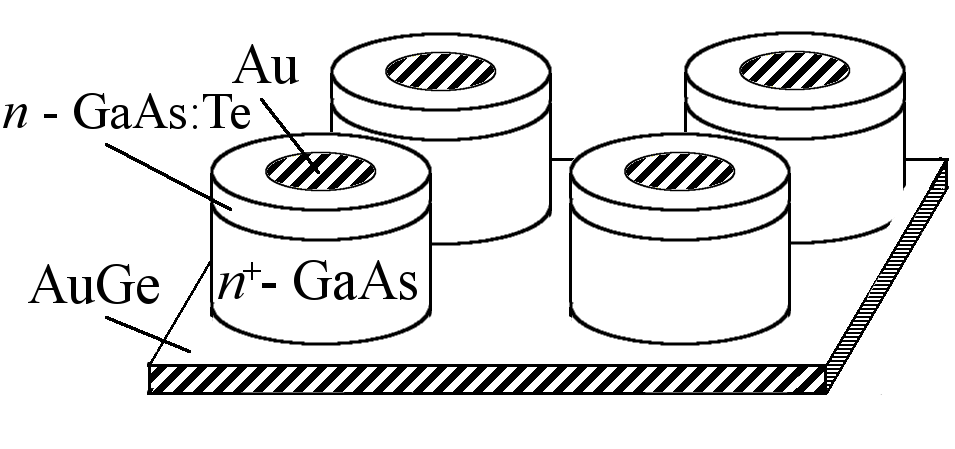
\includegraphics[width=0.9\textwidth]{MSGA}%
\caption{\label{figMSGA}
Структури Au--TiB$_x$--$n$--$n^+$--GaAs.
}
\end{figure}

Діоди були виготовлені по технології з інтегральним тепловідведенням.
Кожен зразок містив близько 20 окремих діодів.
Вимірювання ВАХ кожного з діодів зразка проводилось в темряві при кімнатній температурі
як до, так і після УЗО.

УЗО структур проводились при кімнатних температурах, при цьому в зразках збуджувалися повздовжні АХ.
Обробки проводилися в етиловому спирті, який і використовувався для створення акустичного контакту.
Детальні параметри УЗО наведено в Таблиці~\ref{tabUST}, зокрема там вказано тривалість $t_\mathtt{UST}$ впливу пружних коливань
Так як УЗО викликали незворотні зміни параметрів ДШ, то обробка кожного зі зразків проводилася лише з використанням однієї частоти.

\begin{table}
\caption{\label{tabUST}Параметри ультразвукових обробок структур Au--TiB$_x$--$n$--$n^+$--GaAs.
}
\center
\begin{tabular}{|c|c|c|c|c|}
\hline
$f_\mathtt{US}$, МГц&$W_{\mathtt{US}}$, Вт/см$^2$&$T$, K&$t_\mathtt{UST}$, год &Позначення\\
\hline
4,1&0,8&300&5&U04--08\\ \hline
4,1&1,8&300&5&U04--18\\ \hline
4,1&3,1&300&5&U04--31\\ \hline
9,4&0,5&300&5&U09--05\\ \hline
9,4&1,6&300&5&U09--16\\ \hline
30,0&0,3&300&5&U30--03\\ \hline
\end{tabular}
\end{table}


\subsection{Ефекти ультразвукової обробки у структури Au--TiB$_x$--$n$--$n^+$--GaAs}

Прямі ділянки ВАХ апроксимувалися класичним для механізму ТЕ виразом
\begin{equation}\label{eqIVGAMS}
  I=AA^*T^2\exp\left(-\frac{\Phi_b}{kT}\right)\exp\left(\frac{qV}{n_\mathrm{id}kT}\right),
\end{equation}
де стала Річардсона для GaAs $A^*=8,16\cdot10^4$~A$\cdot$м$^{-2}\cdot$K$^{-2}$,
що дозволило визначити ВБШ та фактор неідеальності.
Точність визначення цих параметрів складала $\pm0,01$ та $0,004$~еВ, відповідно.
На Рис.~\ref{figFbn_GA} наведено дані щодо значення величин $\Phi_b$ та $n_\mathrm{id}$
для наборів діодів, які знаходилися на одному зразку, до та після УЗО.



\begin{figure}
\center
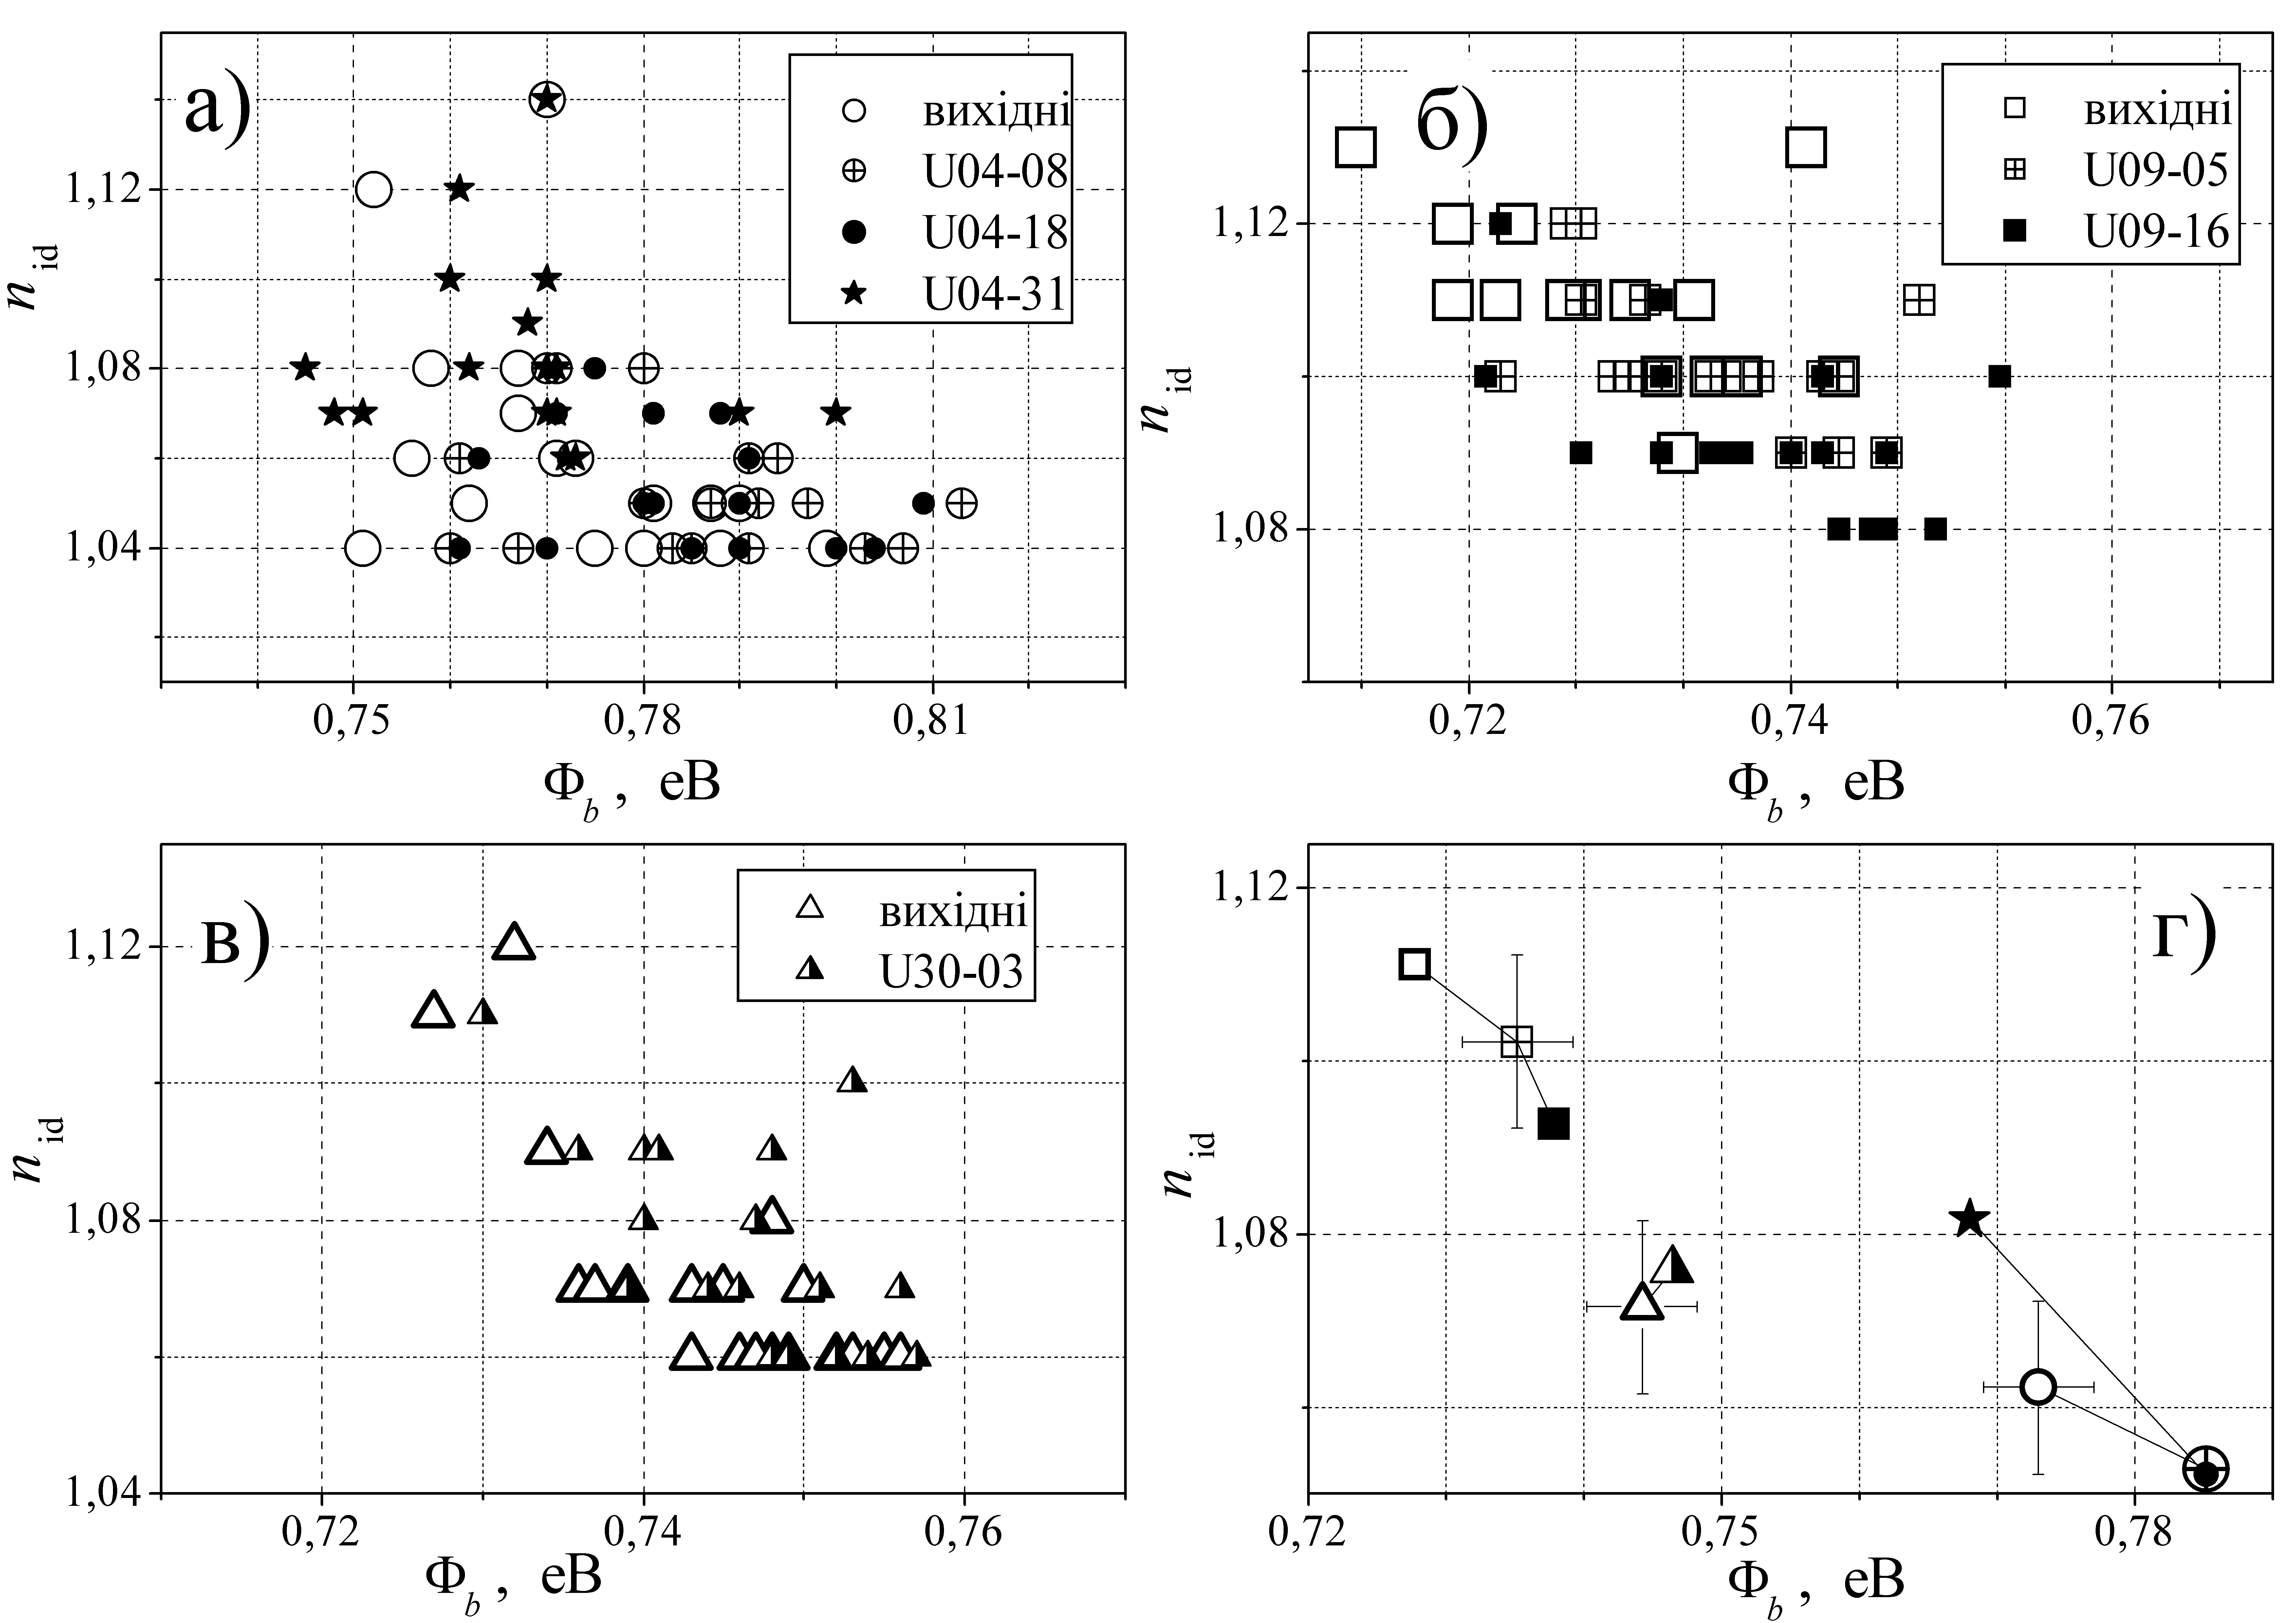
\includegraphics[width=0.95\textwidth]{figFbn_GA}%
\caption{\label{figFbn_GA}
Визначені величини ВБШ та фактору неідеальності для набору структур Au--TiB$_x$--$n$--$n^+$--GaAs
з одного зразка до (порожні точки) та після УЗО.
$f_\mathtt{US}$,~МГц: 4,1 (а), 9,4 (б), 30 (в).
На частині (г) показані середні значення параметрів на наборі діодів з одного зразка,
позначення точок співпадають з попередніми частинами.
}
\end{figure}

Зауважимо, що незважаючи на те, що всі діоди були створені в єдиному технологічному процесі,
існує розкид величин їх параметрів.
Ця ситуація є достатньо типовою --- див., наприклад \cite{SBD:rizn,Milenin1994}.
Як показують наведені дані, внаслідок УЗО з $0,5$~Вт/см$^2\leq W_\mathtt{US}<2,5$~Вт/см$^2$
розкид параметрів дещо зменшився.
Переважно це відбулося завдяки збільшенню висоти бар'єру діодів з меншим вихідним значенням $\Phi_b$ та
зменшення фактору неідеальності ДШ з більшим $n_\mathrm{id}$.
Як наслідок, в середньому по сукупності діодів ВБШ збільшилась приблизно 0,01~еВ, а зменшення $n_\mathrm{id}$ не
перевищило 0,02 --- див. Рис.~\ref{figFbn_GA},г.

Загалом АІ незворотні зміни прямих ділянок ВАХ досить малі.
Так, зокрема, при УЗО з $f_\mathtt{US}=30$~МГц акусто--індукованих змін практично не спостерігалося,
незважаючи на те, що результати, наведені в попередніх розділах показують, що при збільшенні частоти АХ
ефективність ультразвукового впливу, як правило, зростає.
Тобто, в даному випадку визначальним фактором є інтенсивність УЗ, а не частота, і саме тому УЗО U30--03
викликала мінімальні зміни властивостей ДШ.

\begin{figure}
\center
%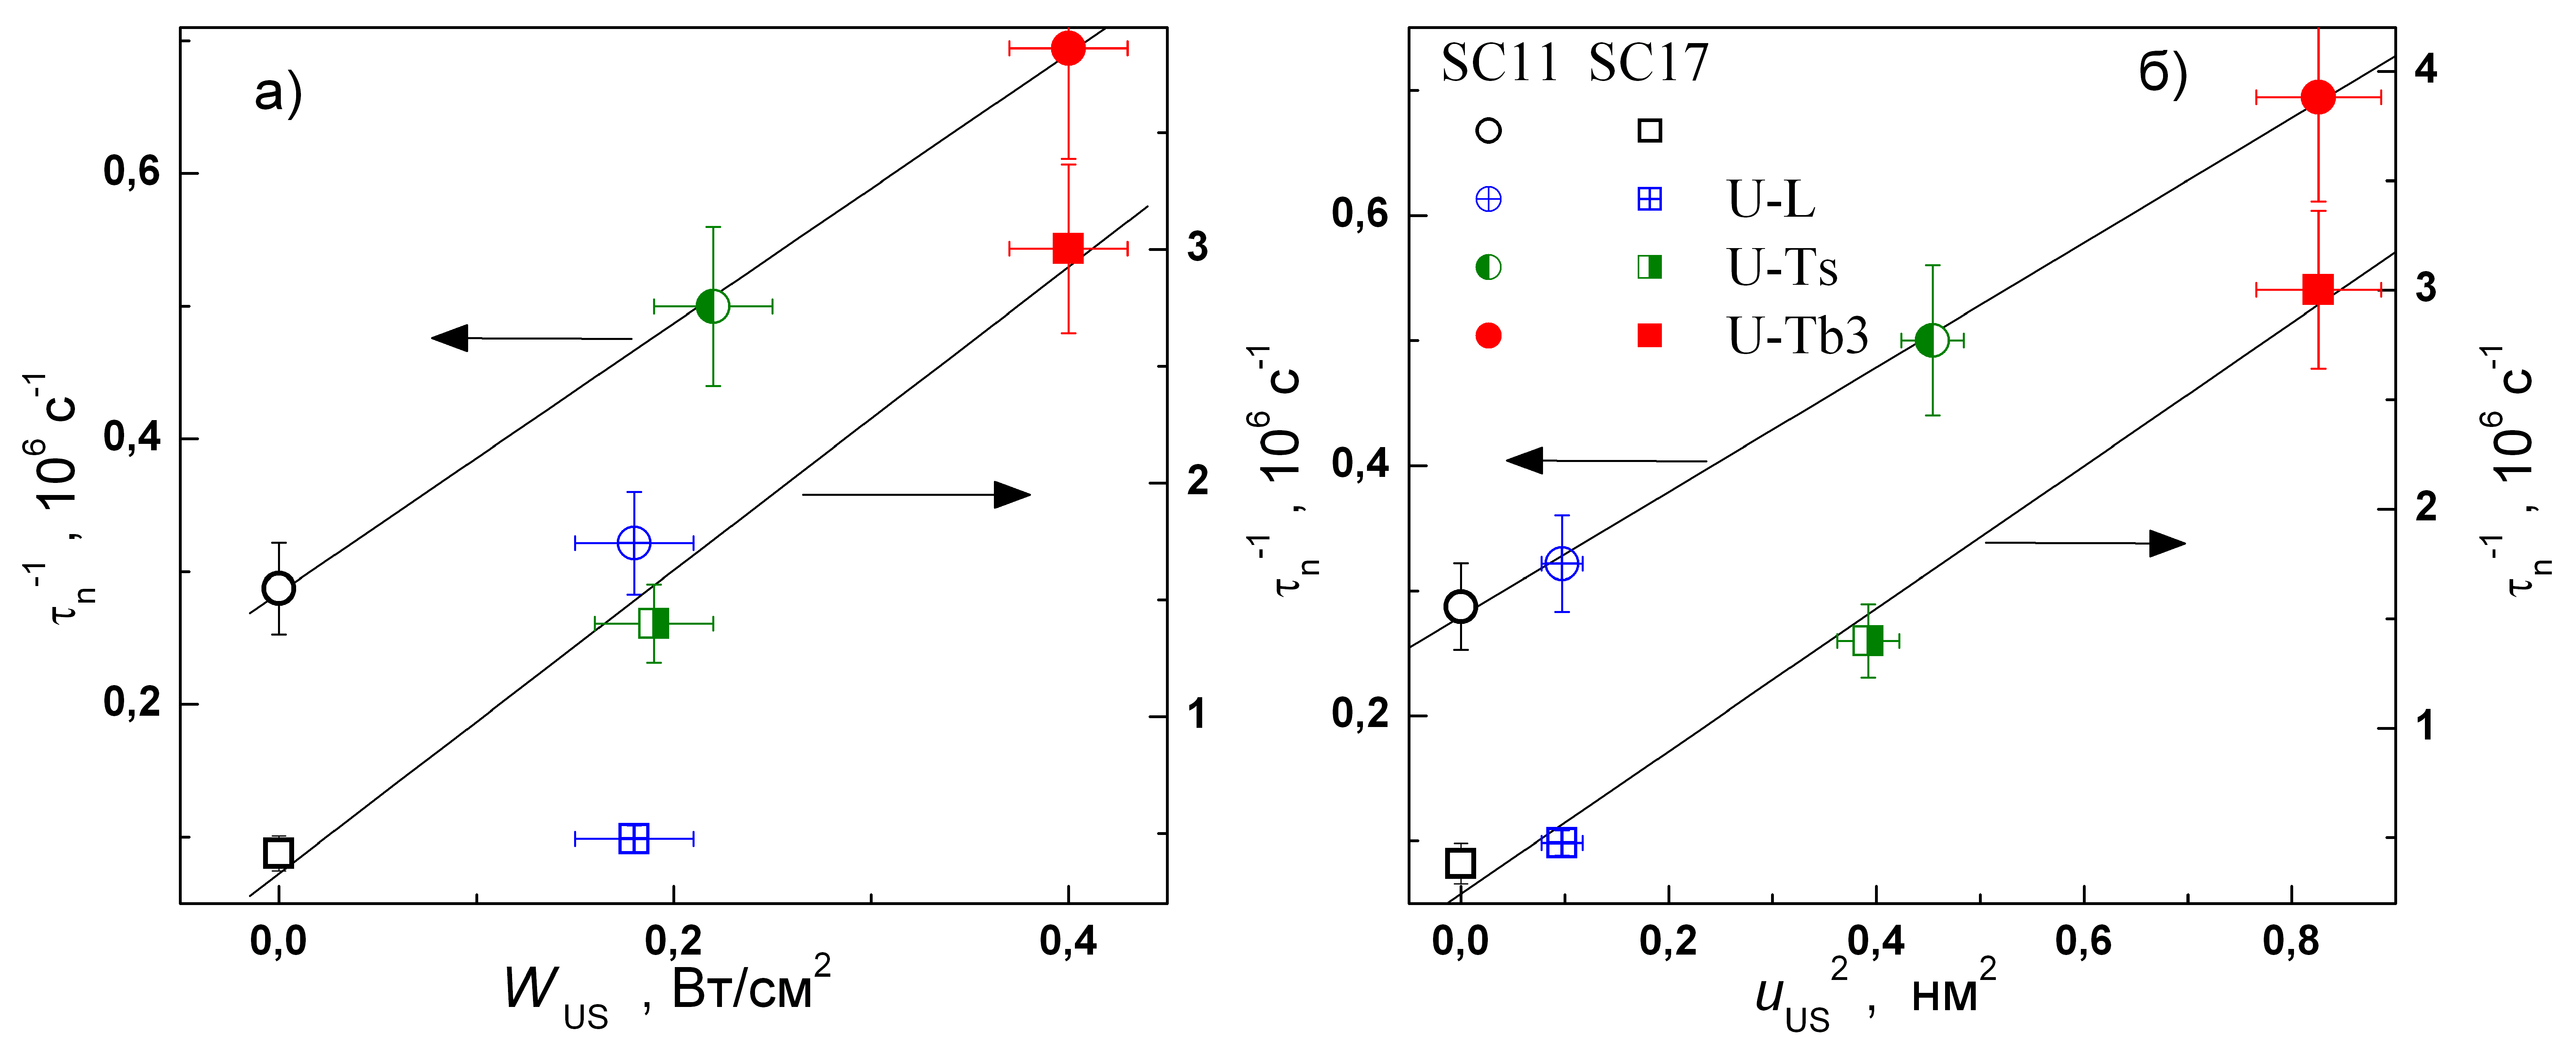
\includegraphics[width=1\textwidth]{figKus}%
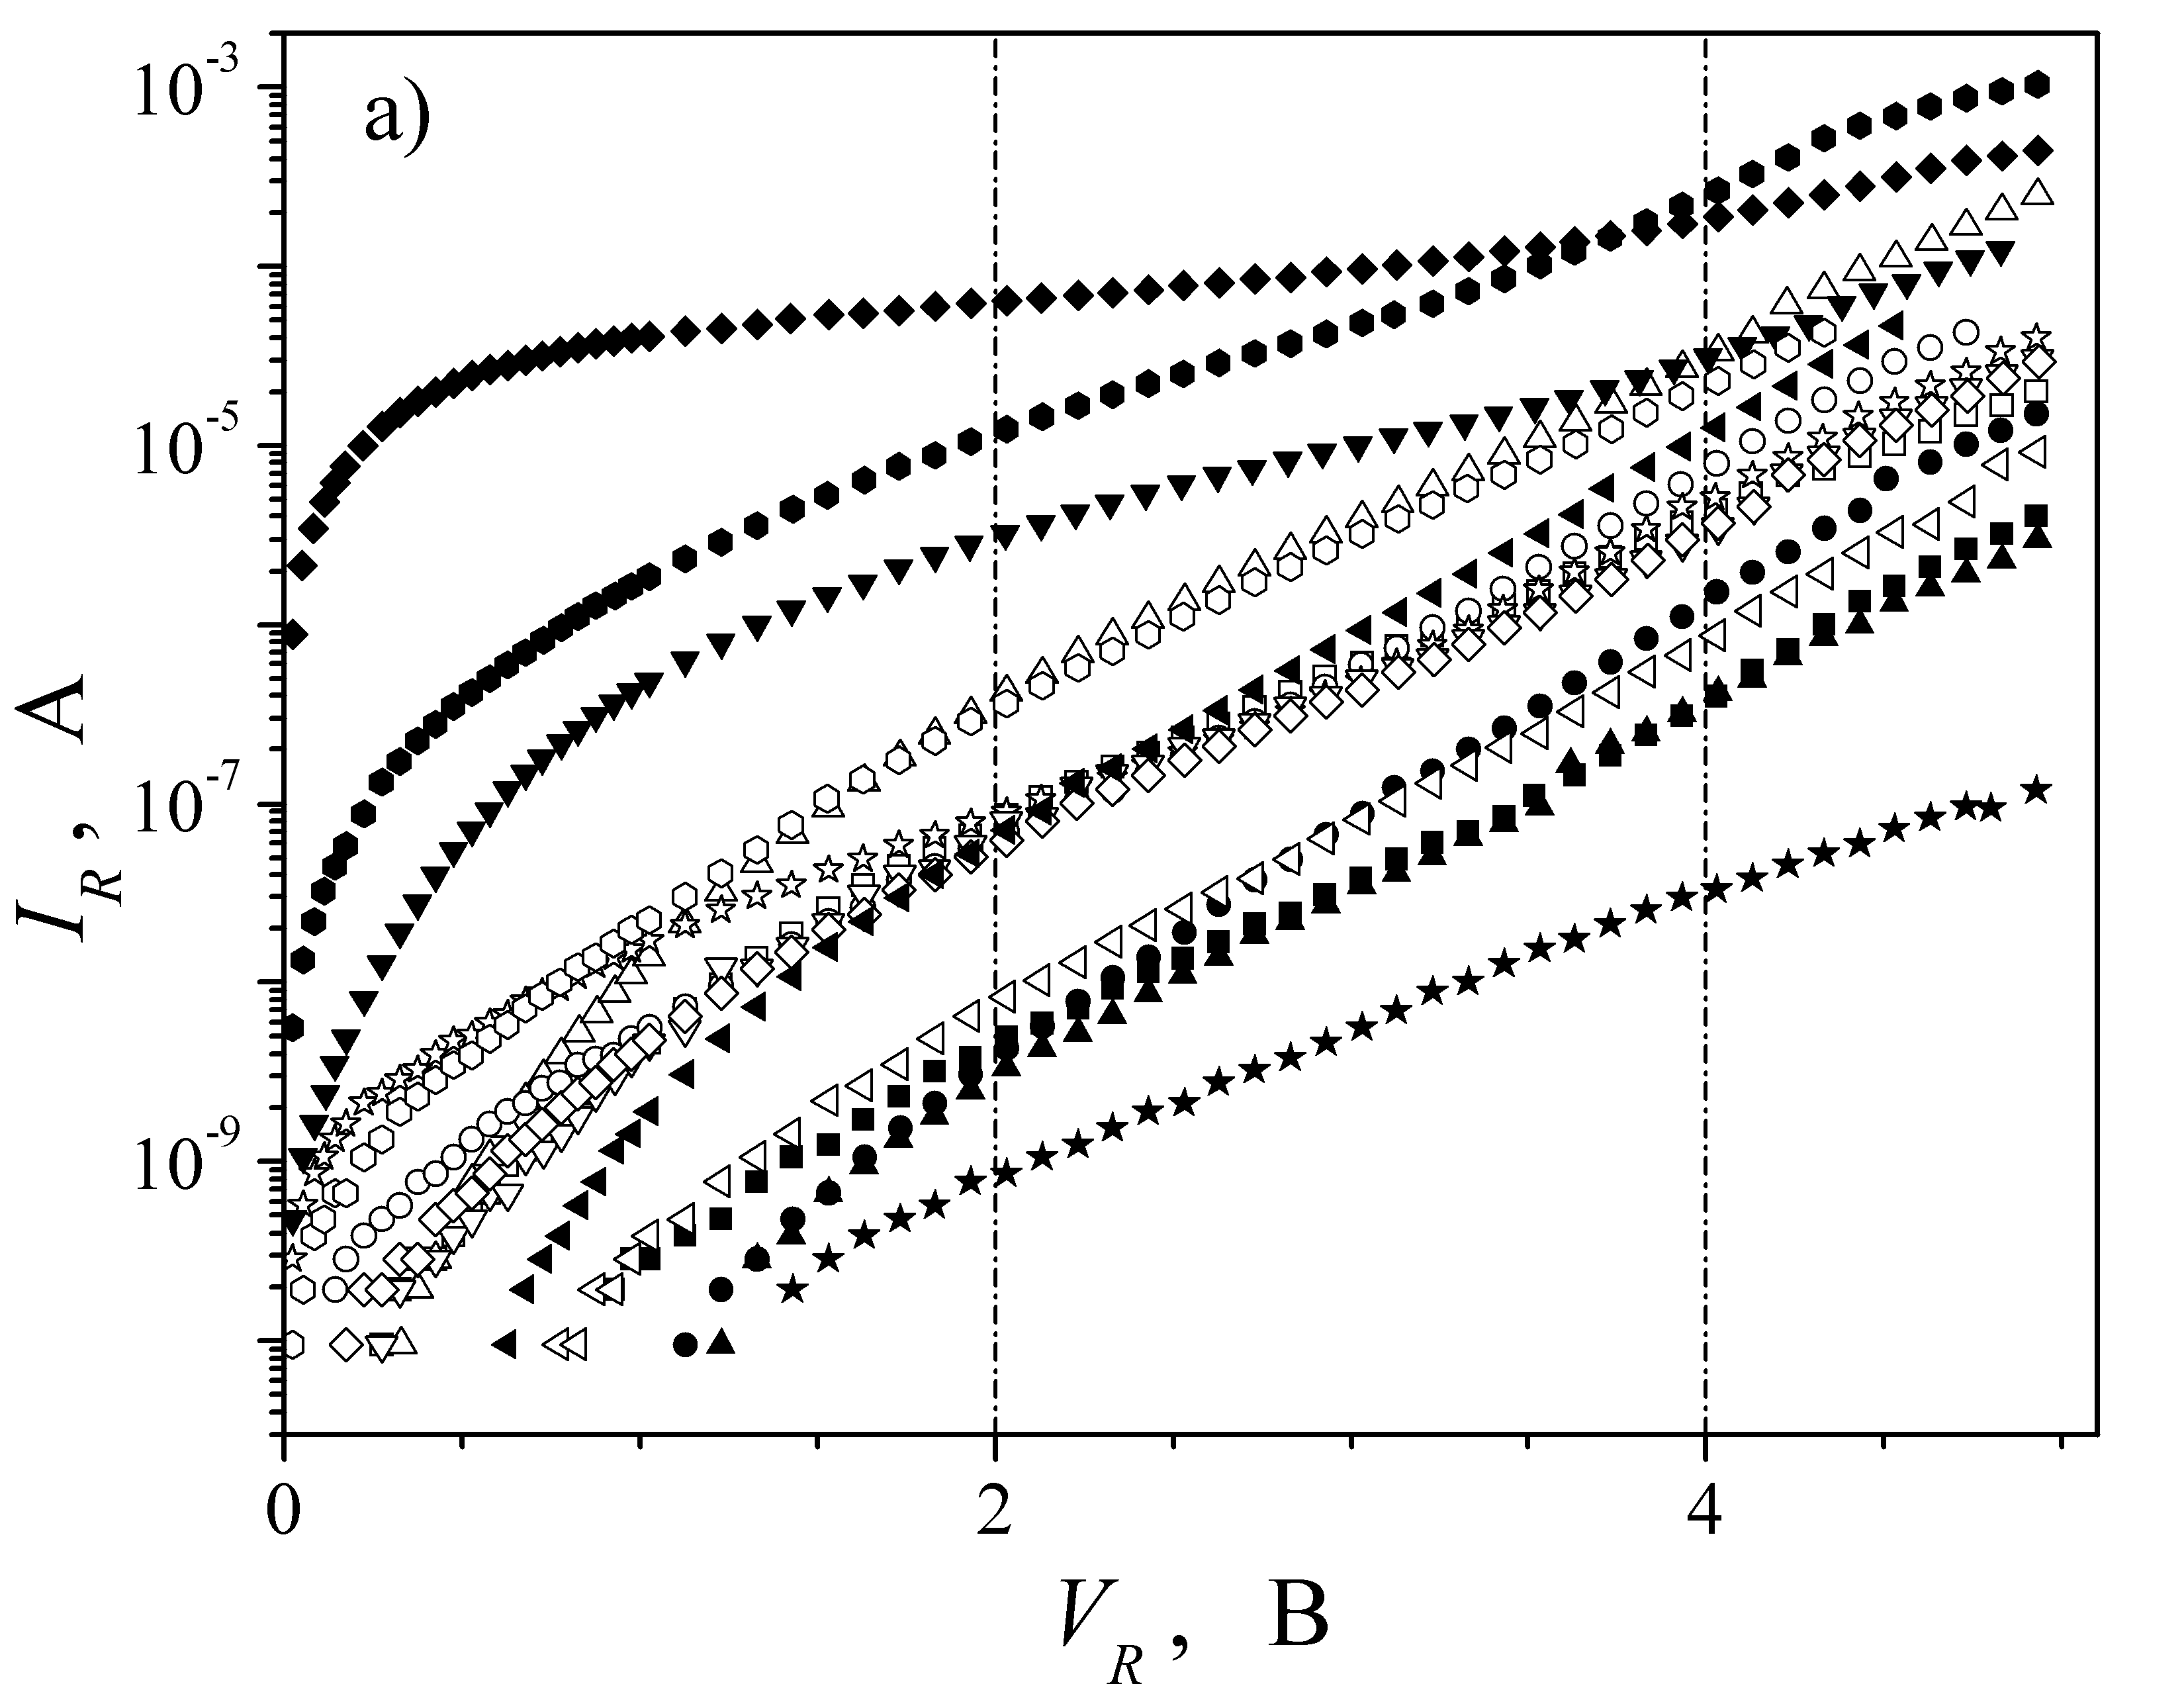
\includegraphics[width=0.49\textwidth]{figIV_GA2} \hfill
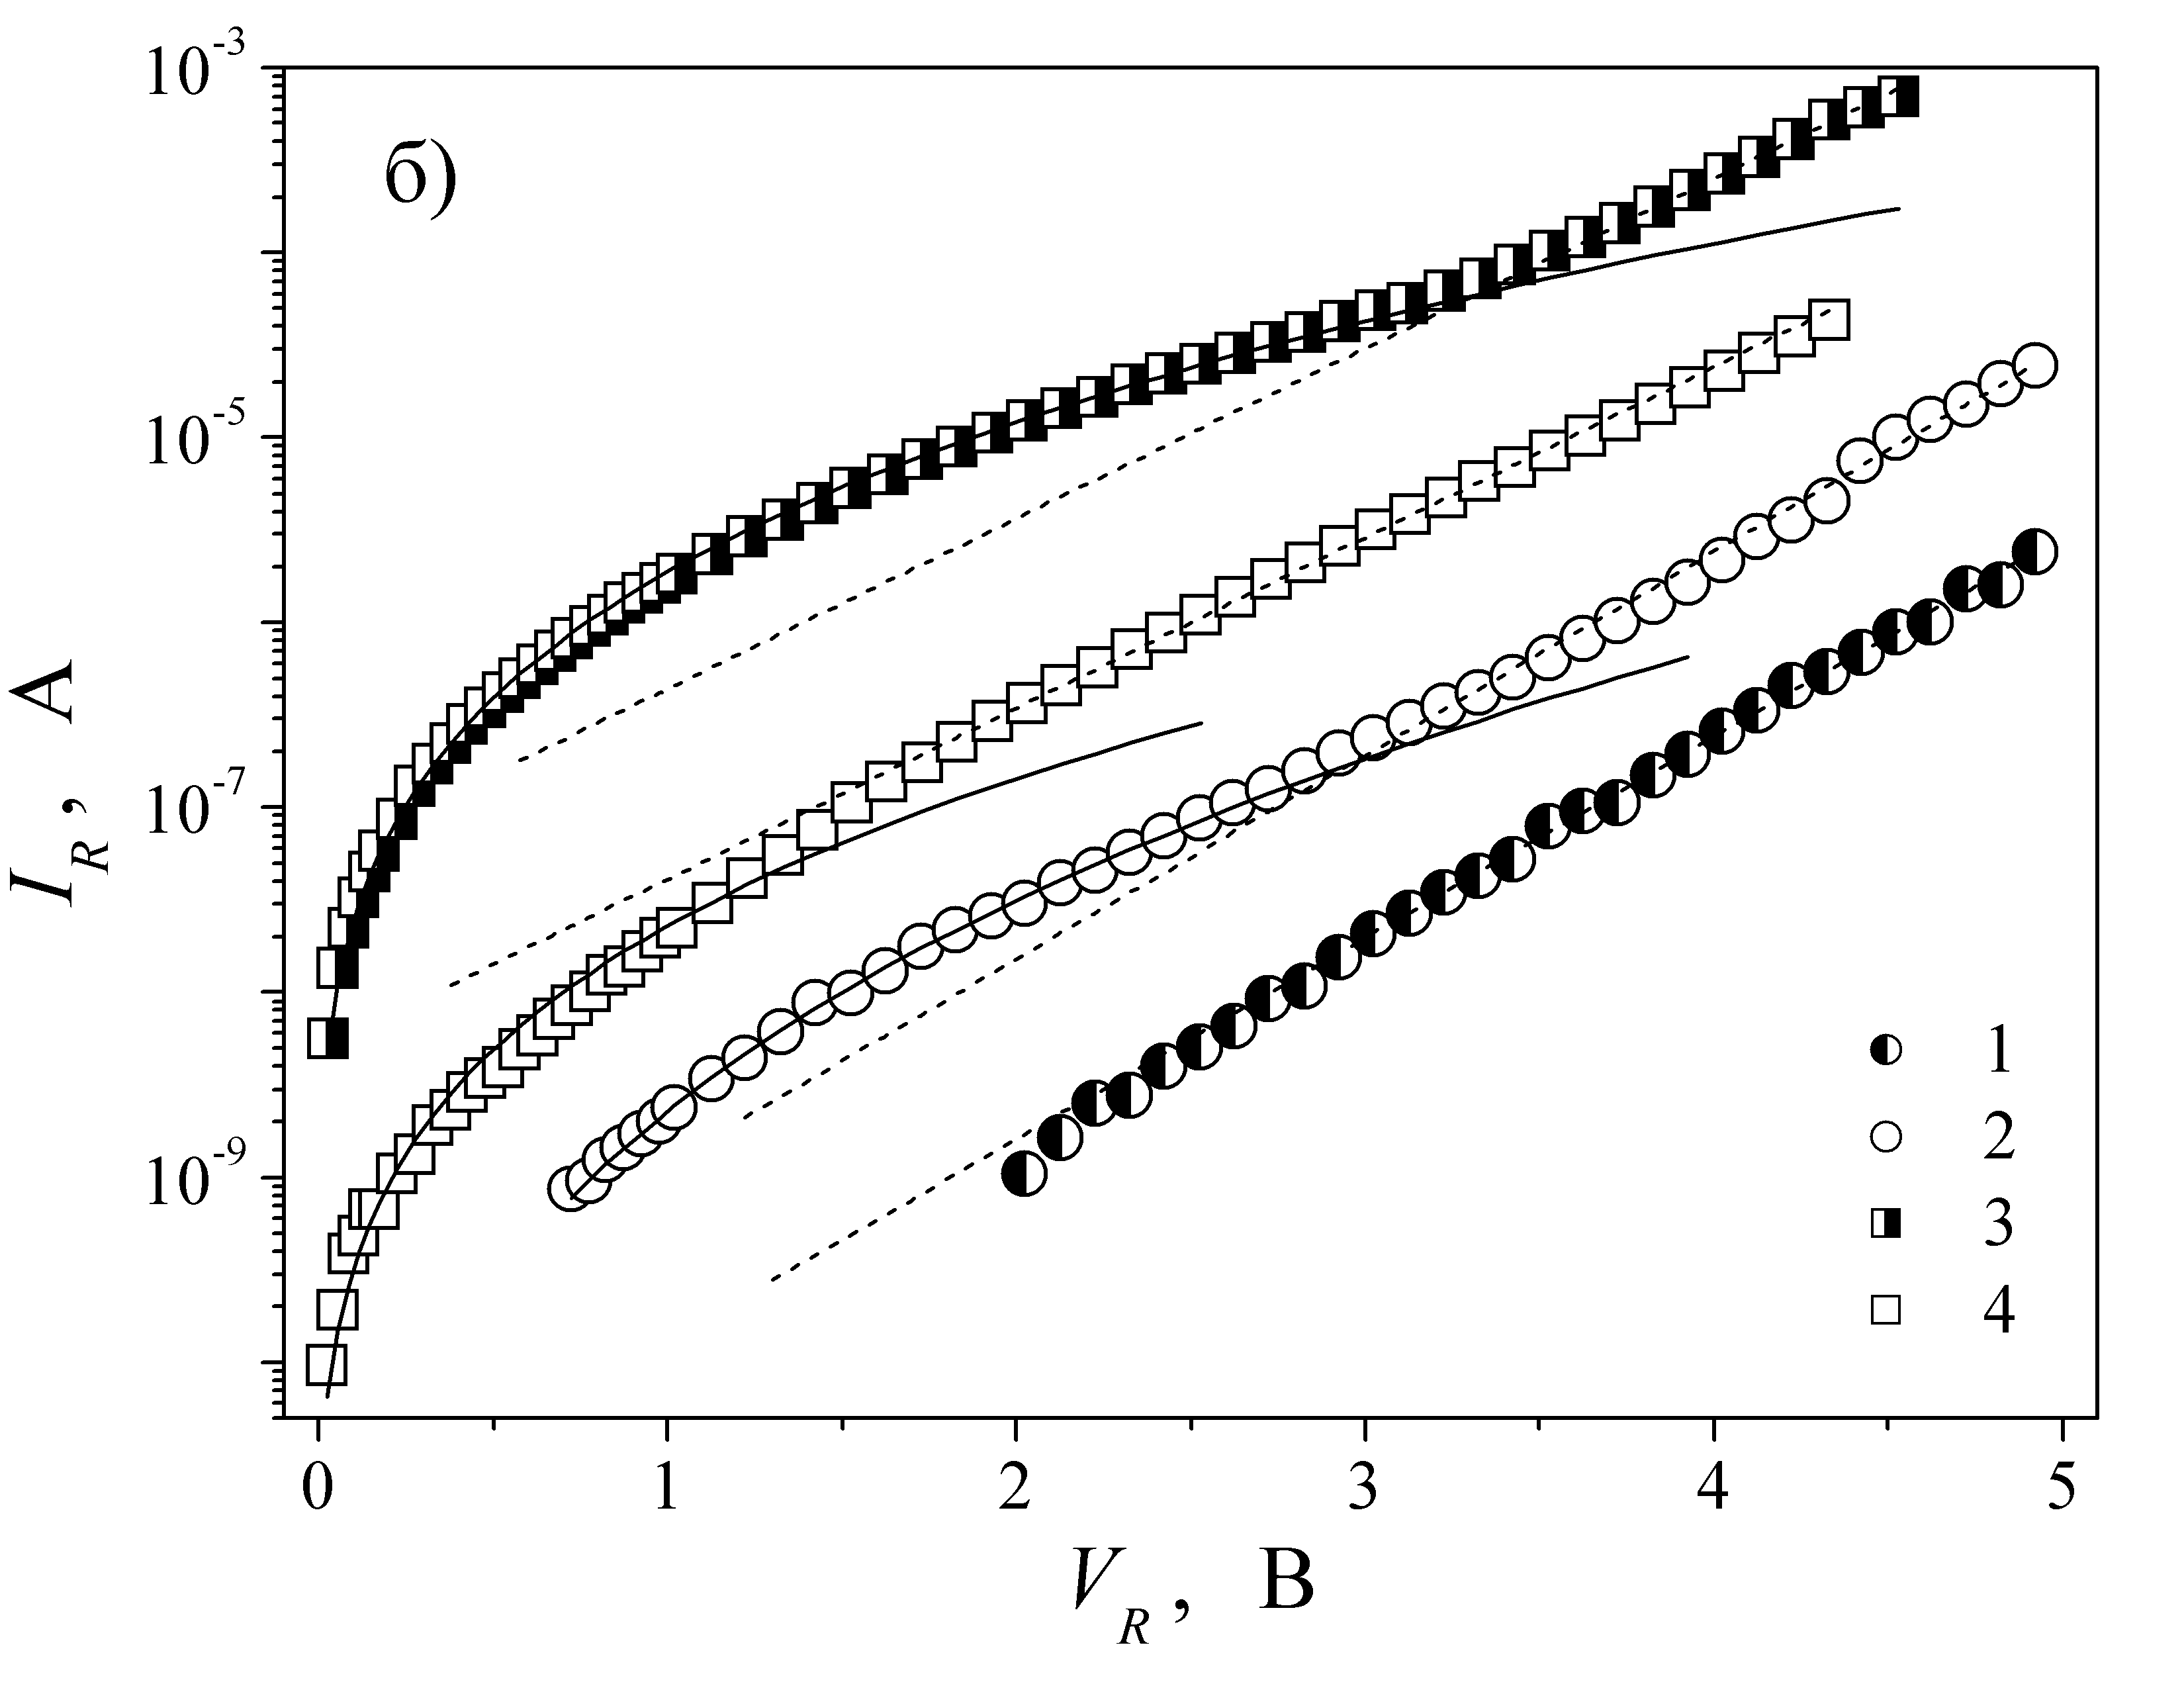
\includegraphics[width=0.49\textwidth]{figIV_GA1}
\caption{\label{figIV_GA}
Зворотні гілки ВАХ структур Au--TiB$_x$--$n$--$n^+$--GaAs
до УЗО (заповнені та напівзаповнені точки)
та після U04--18 (порожні точки).
Точки однакової форми відповідають однаковим діодам.
На рисунку (а) наведено криві, отримані для частини набору структур з одного зразка,
на рисунку (б) --- типові залежності для діодів з високим (3, 4) та низьким (1, 2)
вихідним струмом.
Суцільні лінії --- апроксимація частини ВАХ згідно з формулою~(\ref{eqIR2:GA}),
пунктирні  --- згідно з (\ref{eqIR1:GA}).
$I_{s,\mathtt{tun}}$, A: $1,4\cdot10^{-15}$ (1), $4,7\cdot10^{-15}$ (2), $2,7\cdot10^{-11}$ (3), $5,2\cdot10^{-12}$ (4);
$a_\mathtt{tun}$, В$^{-1/2}$: 9,5 (1), 9,7 (2), 10,5 (3), 10,1 (4).
}%
\end{figure}

З іншого боку, залежність АІ змін від $W_\mathtt{US}$ є немонотонною функцією.
При перевищенні інтенсивністю певного порогу (близько $2,5\div3$~Вт/см$^2$) АІ зміни параметрів набувають
протилежного характеру:  ВБШ зменшується, а фактор неідеальності зростає.
Подібні залежності є досить типовими для УЗО напівпровідників \cite{Zdeb1989,Zaver,Zaver2005}
і пов'язуються, як правило з генерацією дефектів АХ з надпороговою інтенсивністю.



Виміри зворотних гілок ВАХ показали, що розкид параметрів спостерігається і в цьому випадку ---
див. Рис.~\ref{figIV_GA}.
Так, за початковою, до УЗО, величиною зворотного струму $I_R$ досліджені ДШ можна розділити на дві групи.
До першої належать ті, в яких початкові значення зворотного струму невеликі ($I_R<10^{-7}$~А
при $V_R=2$~В) і характер його
польової залежності залишається незмінним у всьому дослідженому інтервалі зміщень.
Діоди другої групи характеризуються більшим значенням струму ($I_R\geq10^{-7}$~А при $V_R=2$~В) та, крім того, на залежності $I_R(V_R)$ спостерігається злам при $V_R>(3\div3,5)$~В.


Вплив УЗО на зворотні гілки ВАХ, по--перше, виявився суттєво більшим, ніж для прямих ВАХ, та, по--друге,
при допорогових інтенсивностях акустичного навантаження характер АІ змін різниться для діодів вищеозначених груп.
Так, для діодів з невисоким початковим зворотнім струмом після УЗО спостерігається зростання $I_R$ при тому ж значенні прикладеної напруги на $1\div2$ порядки,
тоді як для ДШ з другої групи та сама УЗО спричинює зменшення величини $I_R$ в $10\div500$ разів --- див. Рис.~\ref{figIV_GA}.
Як наслідок, УЗО викликає підвищення однорідності характеристик на всьому масиві діодів.
Ілюстрацією цього є Рис.~\ref{figIrG_GA}, на якому наведено залежність величини частки діодів, для яких зворотній струм знаходиться в певному інтервалі $\nu_\mathtt{SD}$,
від величини цього струму до та після УЗО.
Залежності апроксимовано відповідно до розподілу Гауса, параметри апроксимації приведені у підпису до рисунку.
Як видно з наведених даних, УЗО спричинює певне підвищення середнього значення зворотного струму, проте суттєво
покращує такий важливий технологічний параметр при масовому виготовленні структур як однорідність параметрів (дисперсія зменшується в три рази).

\begin{figure}
\center
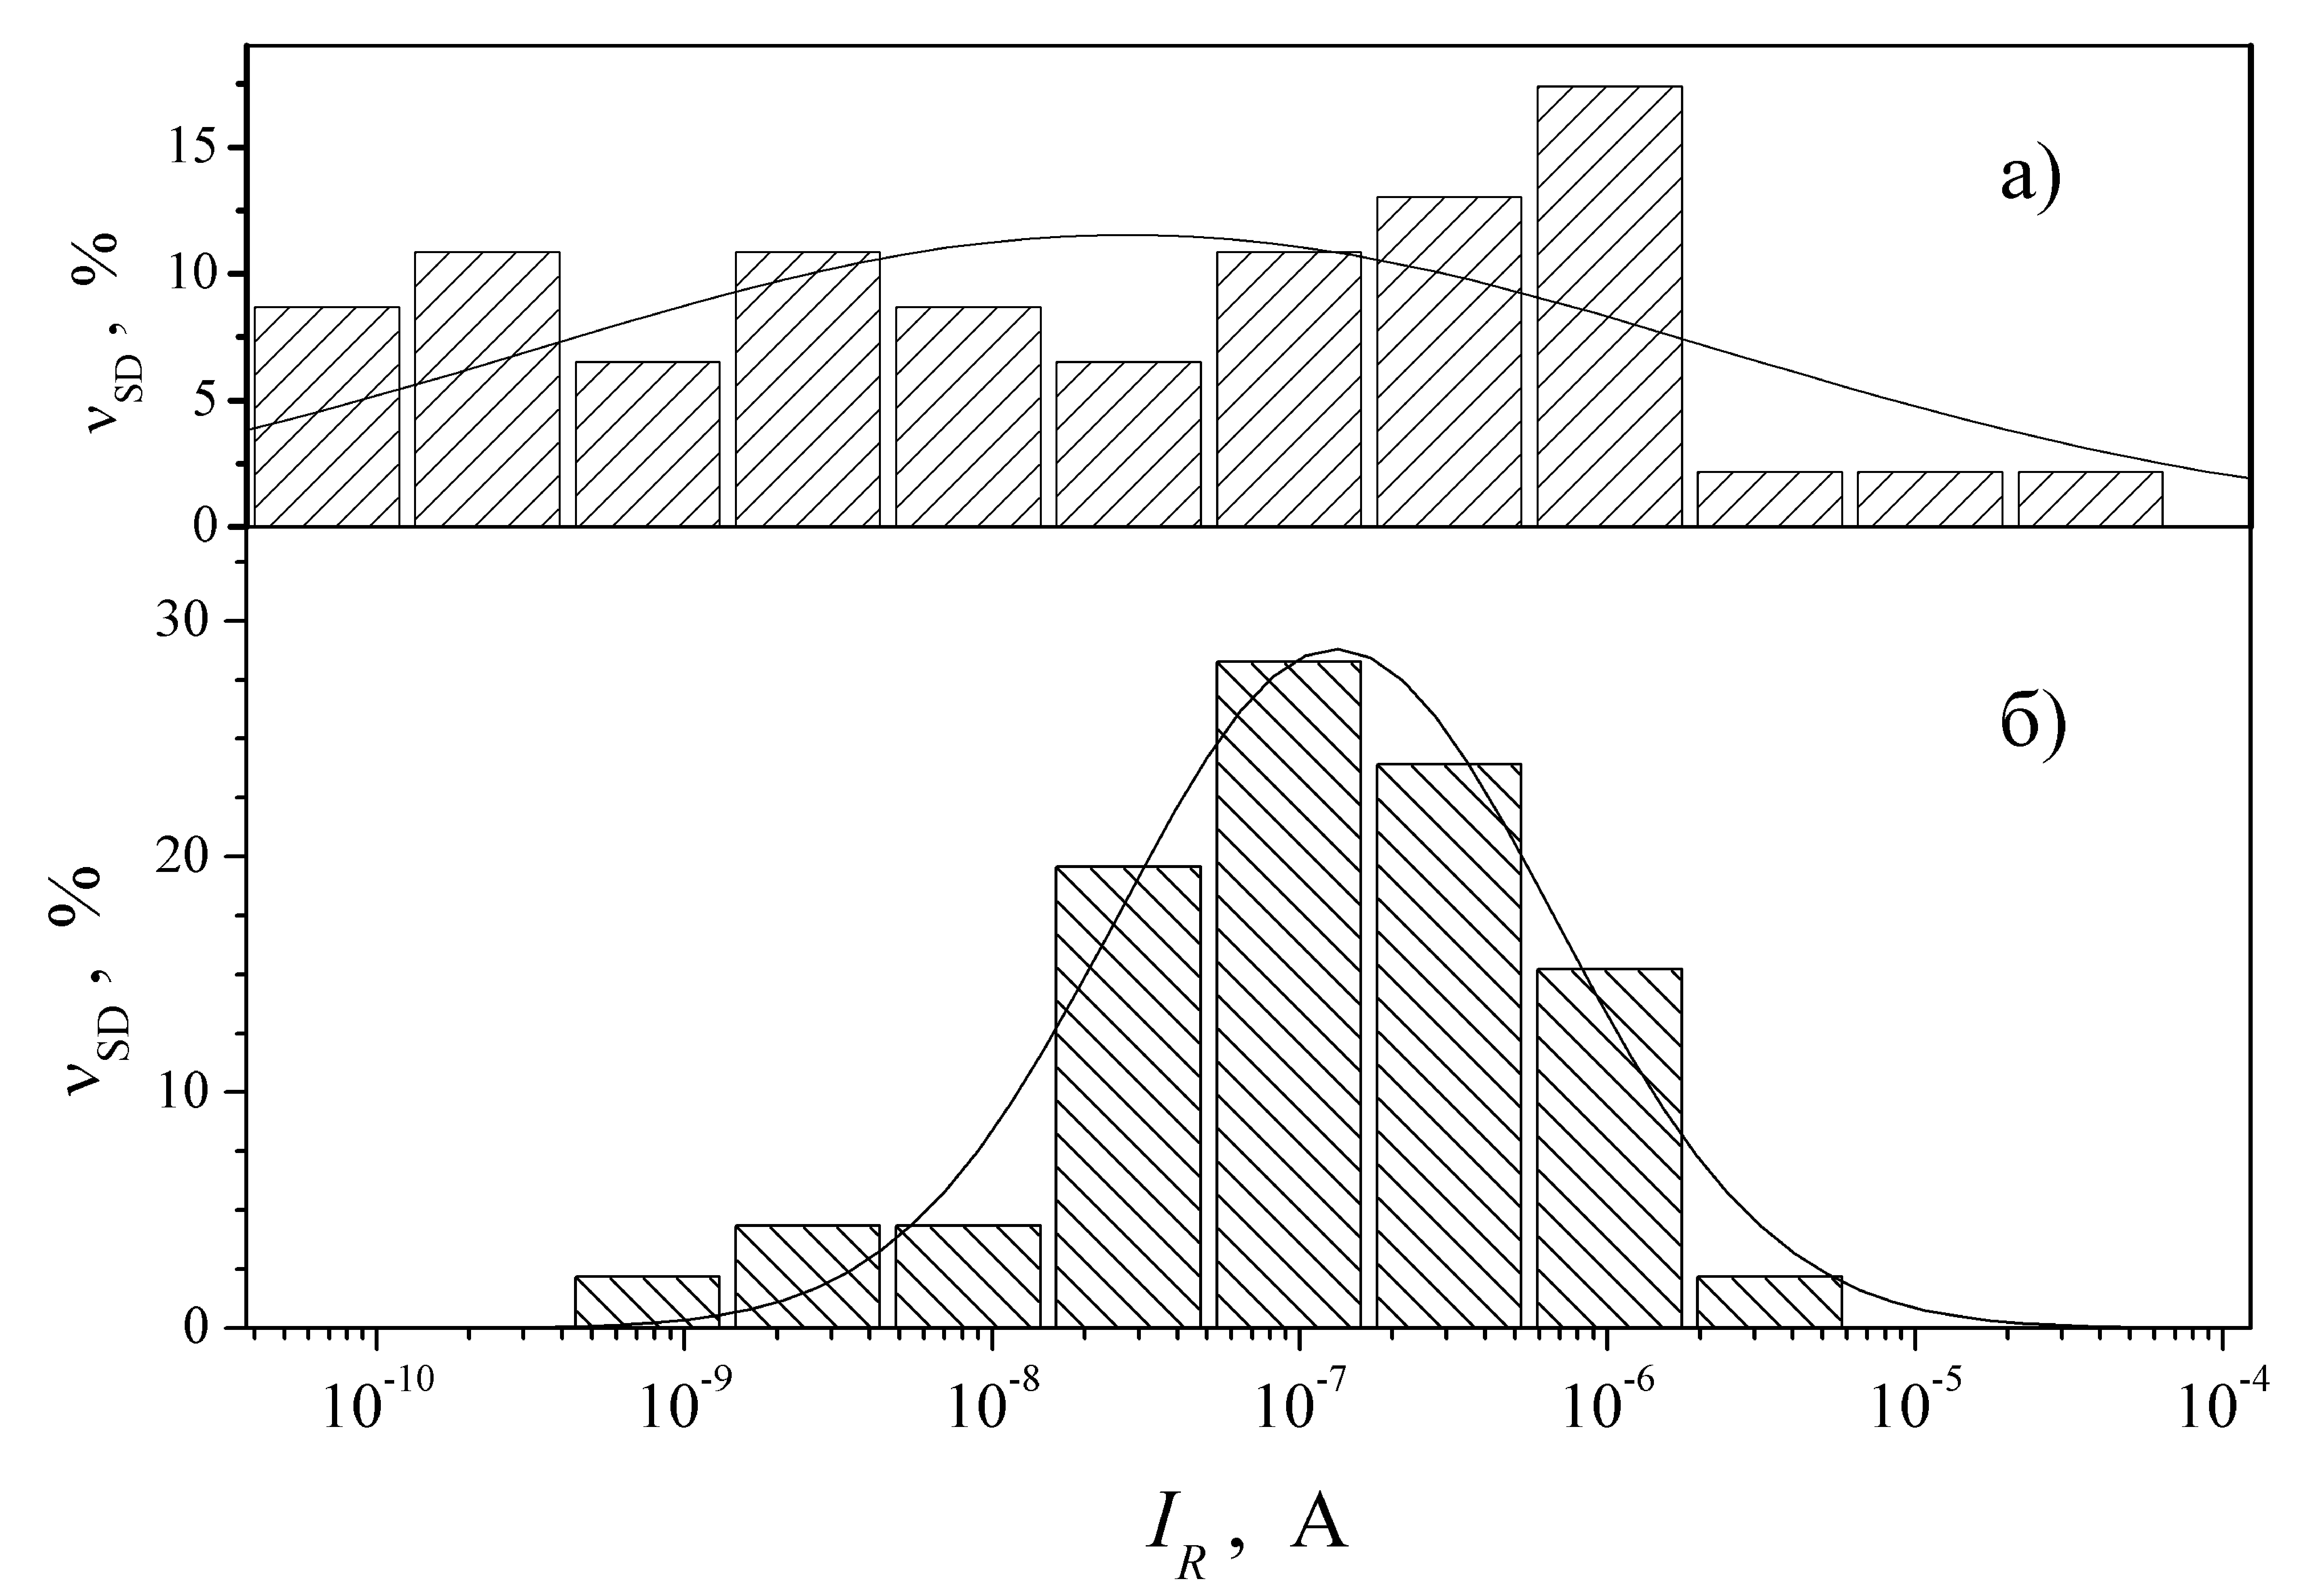
\includegraphics[width=0.75\textwidth]{figIrG_GA}%
\caption{\label{figIrG_GA}
Порівняльні розподіли величини зворотного струму (при $V_R=2$~В)
для структур Au--TiB$_x$--$n$--$n^+$--GaAs до УЗО (а) та після U04--18 і U09--16 (б).
%$W_\mathtt{US}=1,8$~Вт/см$^2$, $f_\mathtt{US}=4,1$~МГц.
По вертикалі відкладена частка діодів, для яких струм знаходиться у відповідному діапазоні.
Загальна кількість діодів --- 40.
Лінії --- апроксимація відповідно до розподілу Гауса.
Середнє значення, А:
$(2,8\pm0,2)\cdot10^{-8}$ (а),
$(1,31\pm0,01)\cdot10^{-7}$ (б).
Дисперсія:
$9\pm2$ (а),
$3,3\pm0,2$ (б).
}
\end{figure}


На наш погляд, протилежні АІ зміни $I_R$ пов’язані з відмінністю переважаючого механізму перенесення заряду через бар'єр в діодах різних груп.
Так, для першої групи залежність зворотного струму від $V_R^{1/2}$ у напівлогарифмічному масштабі є практично прямою лінією --- див. Рис.~\ref{figIV_GA},б, крива 1.
Тобто ВАХ описується виразом
\begin{equation}\label{eqIR1:GA}
I_R=I_{s,\mathtt{tun}}\exp\left(a_\mathtt{tun}V_R^{1/2}\right),
\end{equation}
де
$I_{s,\mathtt{tun}}$ та $a_\mathtt{tun}$ певні константи.
Подібна залежність характерна для тунельного механізму струмоперенесення \cite{Rhoderick1988}.
Проте згідно з класичною теорією Падовані--Стреттона (див., наприклад \cite{Rhoderick1988,Singh1994}) польова або термопольова емісія відіграють
переважаючу роль при $kT\leq qE_{00}^\mathrm{TFE}$,
де $E_{00}^\mathrm{TFE}$ визначається формулою~(\ref{eqE00:TFE}).
Проведені розрахунки показали, що для нашого випадку ($m^*=0,067\cdot9,11\cdot10^{-31}$~кг,
$\varepsilon_s=12,4$, $N_d=6\cdot10^{21}$~м$^{-3}$) $qE_{00}^\mathrm{TFE}\approx1,6\cdot10^{-6}$~еВ.
Таким чином, термопольовою, а тим більше польовою емісією пояснювати зворотній струм в даних діодах не можна.
З іншого боку, з літератури \cite{Evstropov,Evstropov2000,Ganichev:2000,PipinsFTP,Pipinys1999} відомо, що у структурах МН тунелювання може відбуватися за участю енергетичних рівнів, пов'язаних з дефектами в ОПЗ.
Зокрема, у випадку реалізації механізму, запропонованого в роботах \cite{Evstropov,Evstropov2000}, струм проходить внаслідок переміщення електронів
крізь потенціальний бар'єр по люнцюжку глибоких центрів, причиною появи яких можуть бути дислокаційні лінії.
При тунелюванні за участю дефектів $I_{s,\mathtt{tun}}$ визначається, насамперед, від концентрації дефектів,
а $a_\mathtt{tun}$ залежить від їх типу.

Для ДШ другої групи, то залежність $\ln I_R$ від зворотної напруги при малих зміщеннях ($V_R<2.5$~В) суттєво нелінійна
і лише при збільшенні зворотньої напруги починає мати вигляд, характерний для тунельного механізму струмоперенесення.
При невеликих напругах отримані експериментальні дані добре апроксимуються (Рис.~\ref{figIV_GA},б, крива 3) залежністю
\begin{equation}\label{eqIR2:GA}
I_R=I_{s,\mathtt{TE}}\exp\left(a_\mathtt{TE}V_R^{1/4}\right).
\end{equation}
Як відомо \cite{Rhoderick1988},
така залежність характерна для ТЕ струмоперенесення, коли висота бар’єру змінюється під дією сил зображення.
Досить великі абсолютні значення зворотного струму можуть бути пов’язані як з наявністю енергетичних станів на границі розділу \cite{Singh1994,Tseng1987}, так і з неоднорідністю по площі контакту метал-напівпровідник \cite{Askerov:PhD}.
Таким чином, у діодах другої групи при малих зворотних напругах переважаючим механізмом перенесення заряду є термоемісійний, а при зростанні напруженості електричного поля на границі основним механізмом стає тунелювання, зв'язане з дефектами.

УЗО окрім зміни абсолютної величини зворотного струму викликала також і певну модифікацію залежності $I_R(V_R)$.
А саме, у діодах першої групи при невеликих зміщеннях ($V_R<2$~В) ставав помітним внесок термоемісійних процесів (див. Рис.~\ref{figIV_GA},б, крива 2),
тоді як ДШ з першої групи тунелювання ставало переважаючим вже при менших значеннях прикладеної напруги (див. криву 4 на Рис.~\ref{figIV_GA},б, у порівнянні з кривою 3).

Пояснення виявлених дефектів може бути наступним.
З літератури  відомо, що внаслідок УЗО відбувається згладжування локальних неоднорідностей границь розділу \cite{Parchinskii2003r} та
часткова релаксація внутрішніх механічних напруг \cite{BritunFTT,Zdeb1989}.
Так як УЗО не викликає зміни  радіусу кривизни та величини відносної деформації приповерхневих кристалічних площин \cite{UST:SDErmol},
то причиною подібних ефектів може бути перерозподіл по товщині напівпровідника легуючих домішок \cite{Zaver} чи дефектів іншого типу \cite{Ostrov2002FTPr}.
Зміни концентрації заряджених дефектів поблизу поверхні контакту МН, у тому числі і захоплених на дислокації, завдяки акусто--стимулюваній дифузії впливають на заселеність енергетичних рівнів на границі розділу, а саме вона є одним з визначальних факторів як для висоти бар’єру \cite{Rhoderick1988,Singh1994},
так і величини фактора неідеальності \cite{Ikoma}.
Наслідком АІ просторового та хімічного впорядкування приконтактної області GaAs є підвищення однорідності розподілу ВБШ.
Тобто, в місці розташування ДШ, де у вихідному стані ВБШ була невелика, спостерігається збільшення висоти бар'єру;
у діодах, де зворотній струм проходив лише внаслідок тунелювання через високе значення $\Phi_b$, має місце зворотна тенденція.
Ці процеси проявляються у неоднаковій зміні ТЕ компоненти зворотного струму.

Водночас збільшення концентрації дефектів в ОПЗ викликає підсилення процесів тунелювання, що відображається у зростанні відповідної компоненти $I_R$
та збільшенні $I_{s,\mathtt{tun}}$.
Зауважимо, що при $f_\mathtt{US}=4,1$~МГц змін величини $a_\mathtt{tun}$ практично не спостерігається --- див. Рис.~\ref{figIV_GA}, Таблицю~\ref{tabUS_GaAs},
що свідчить про незмінність типу дефектів, які приймають участь у тунелюванні.
При збільшенні частоти УЗО нахил залежності $\ln I_R$ від $V_R^{1/2}$  після обробки починає зменшуватись (Таблиця~\ref{tabUS_GaAs}).
Для ілюстрації на Рис.~\ref{figIr30_GA} наведено зворотні гілки ВАХ до та після U30--03.
Наведені дані свідчать, що, незважаючи на невисоку інтенсивність УЗО, при $f_\mathtt{US}=30$~МГц відбувається процеси перебудови центрів, які викликають появу глибоких рівнів у забороненій зоні.
Іншими словами, ці процеси є суттєво частотнозалежними, що, загалом, співпадає з результатами, представленими у попередній розділах.


\begin{figure}
\center
%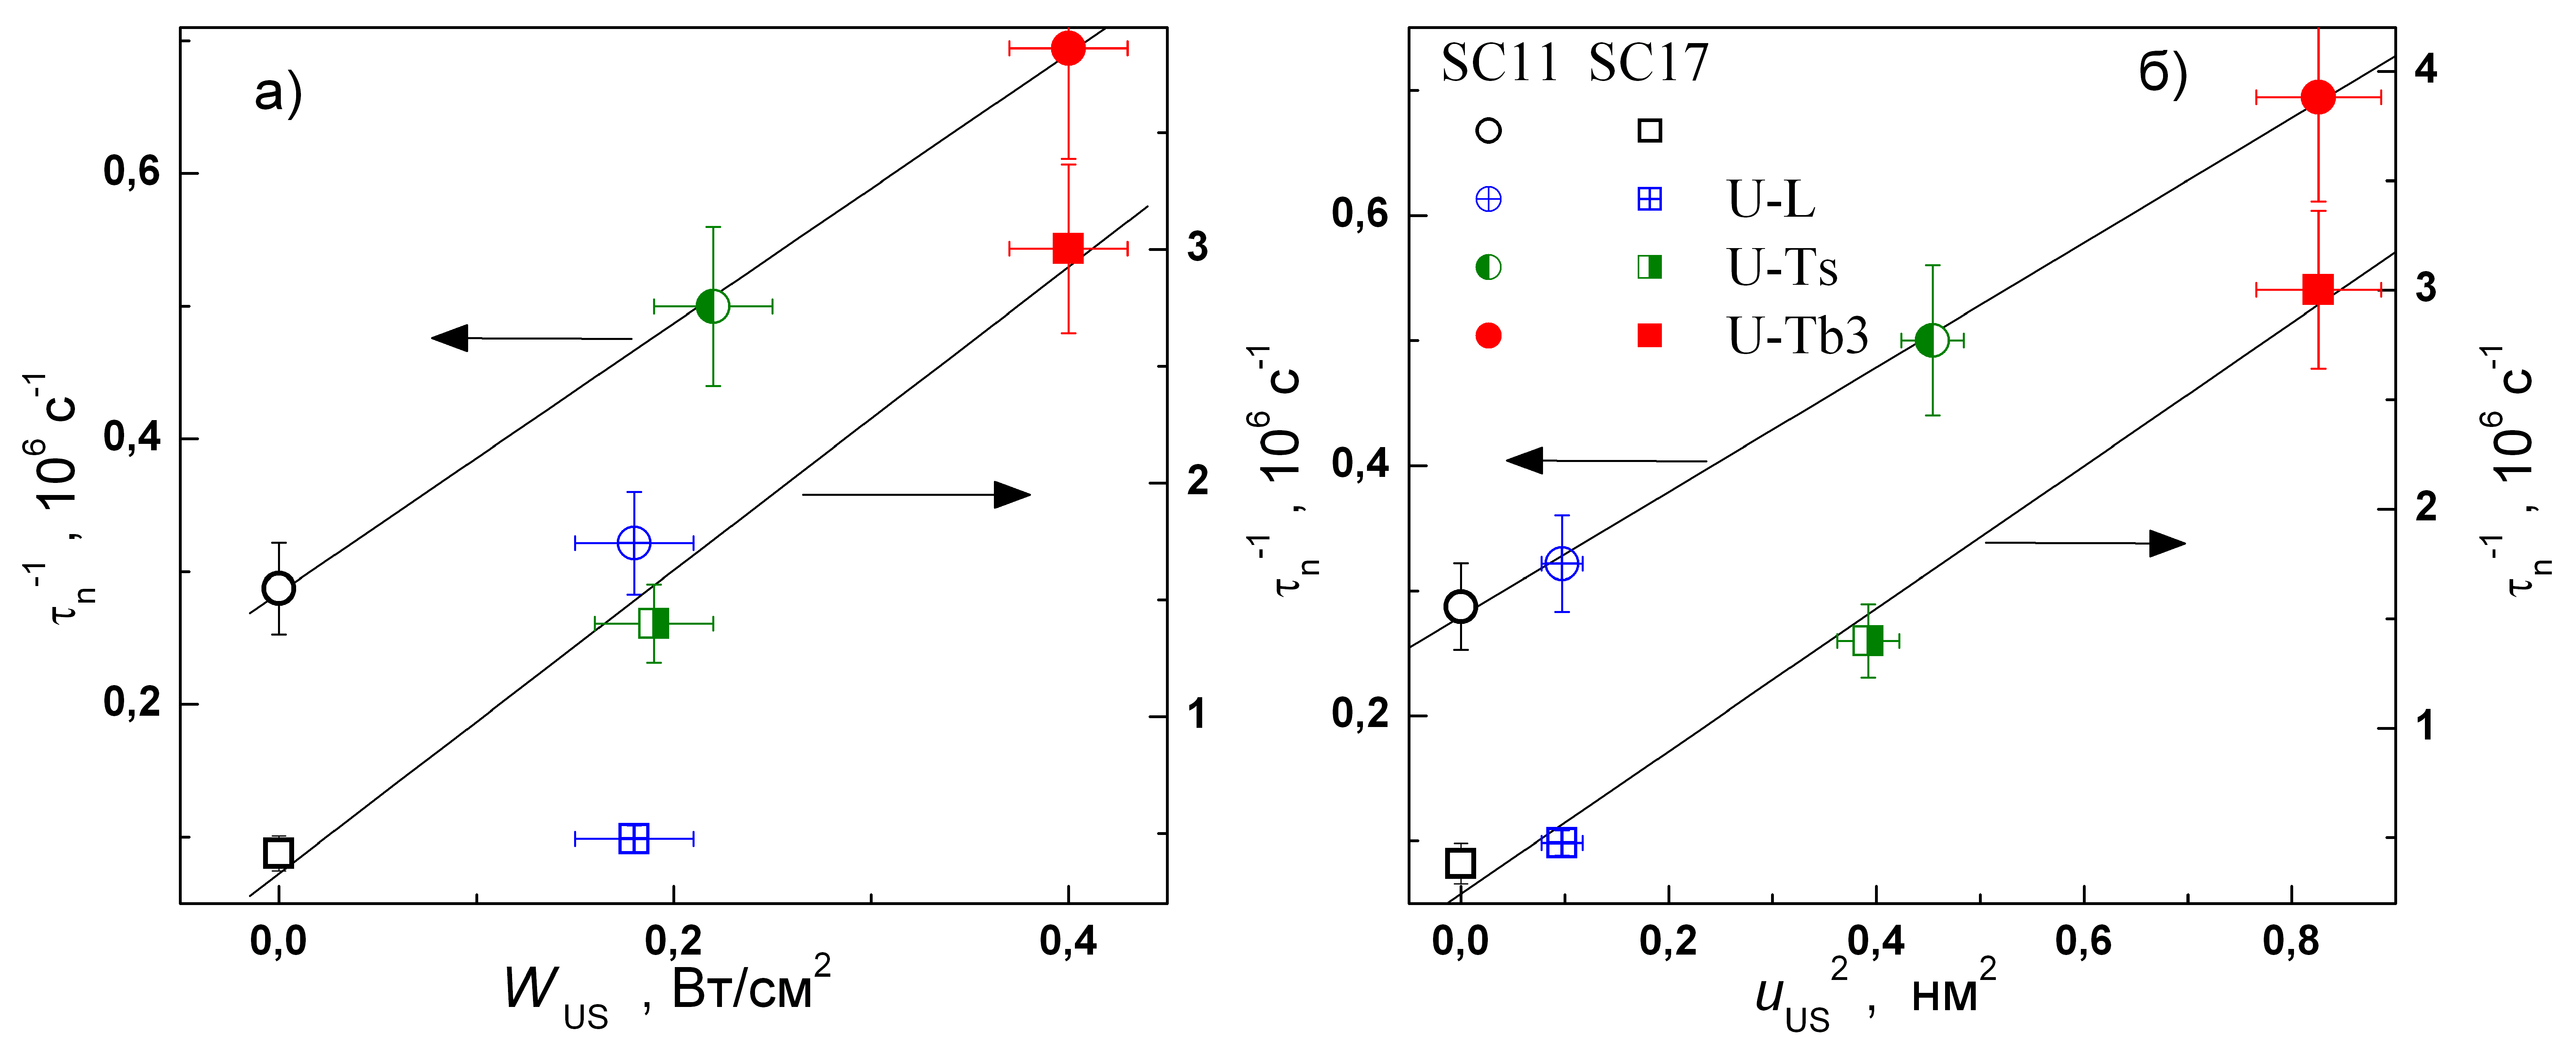
\includegraphics[width=1\textwidth]{figKus}%
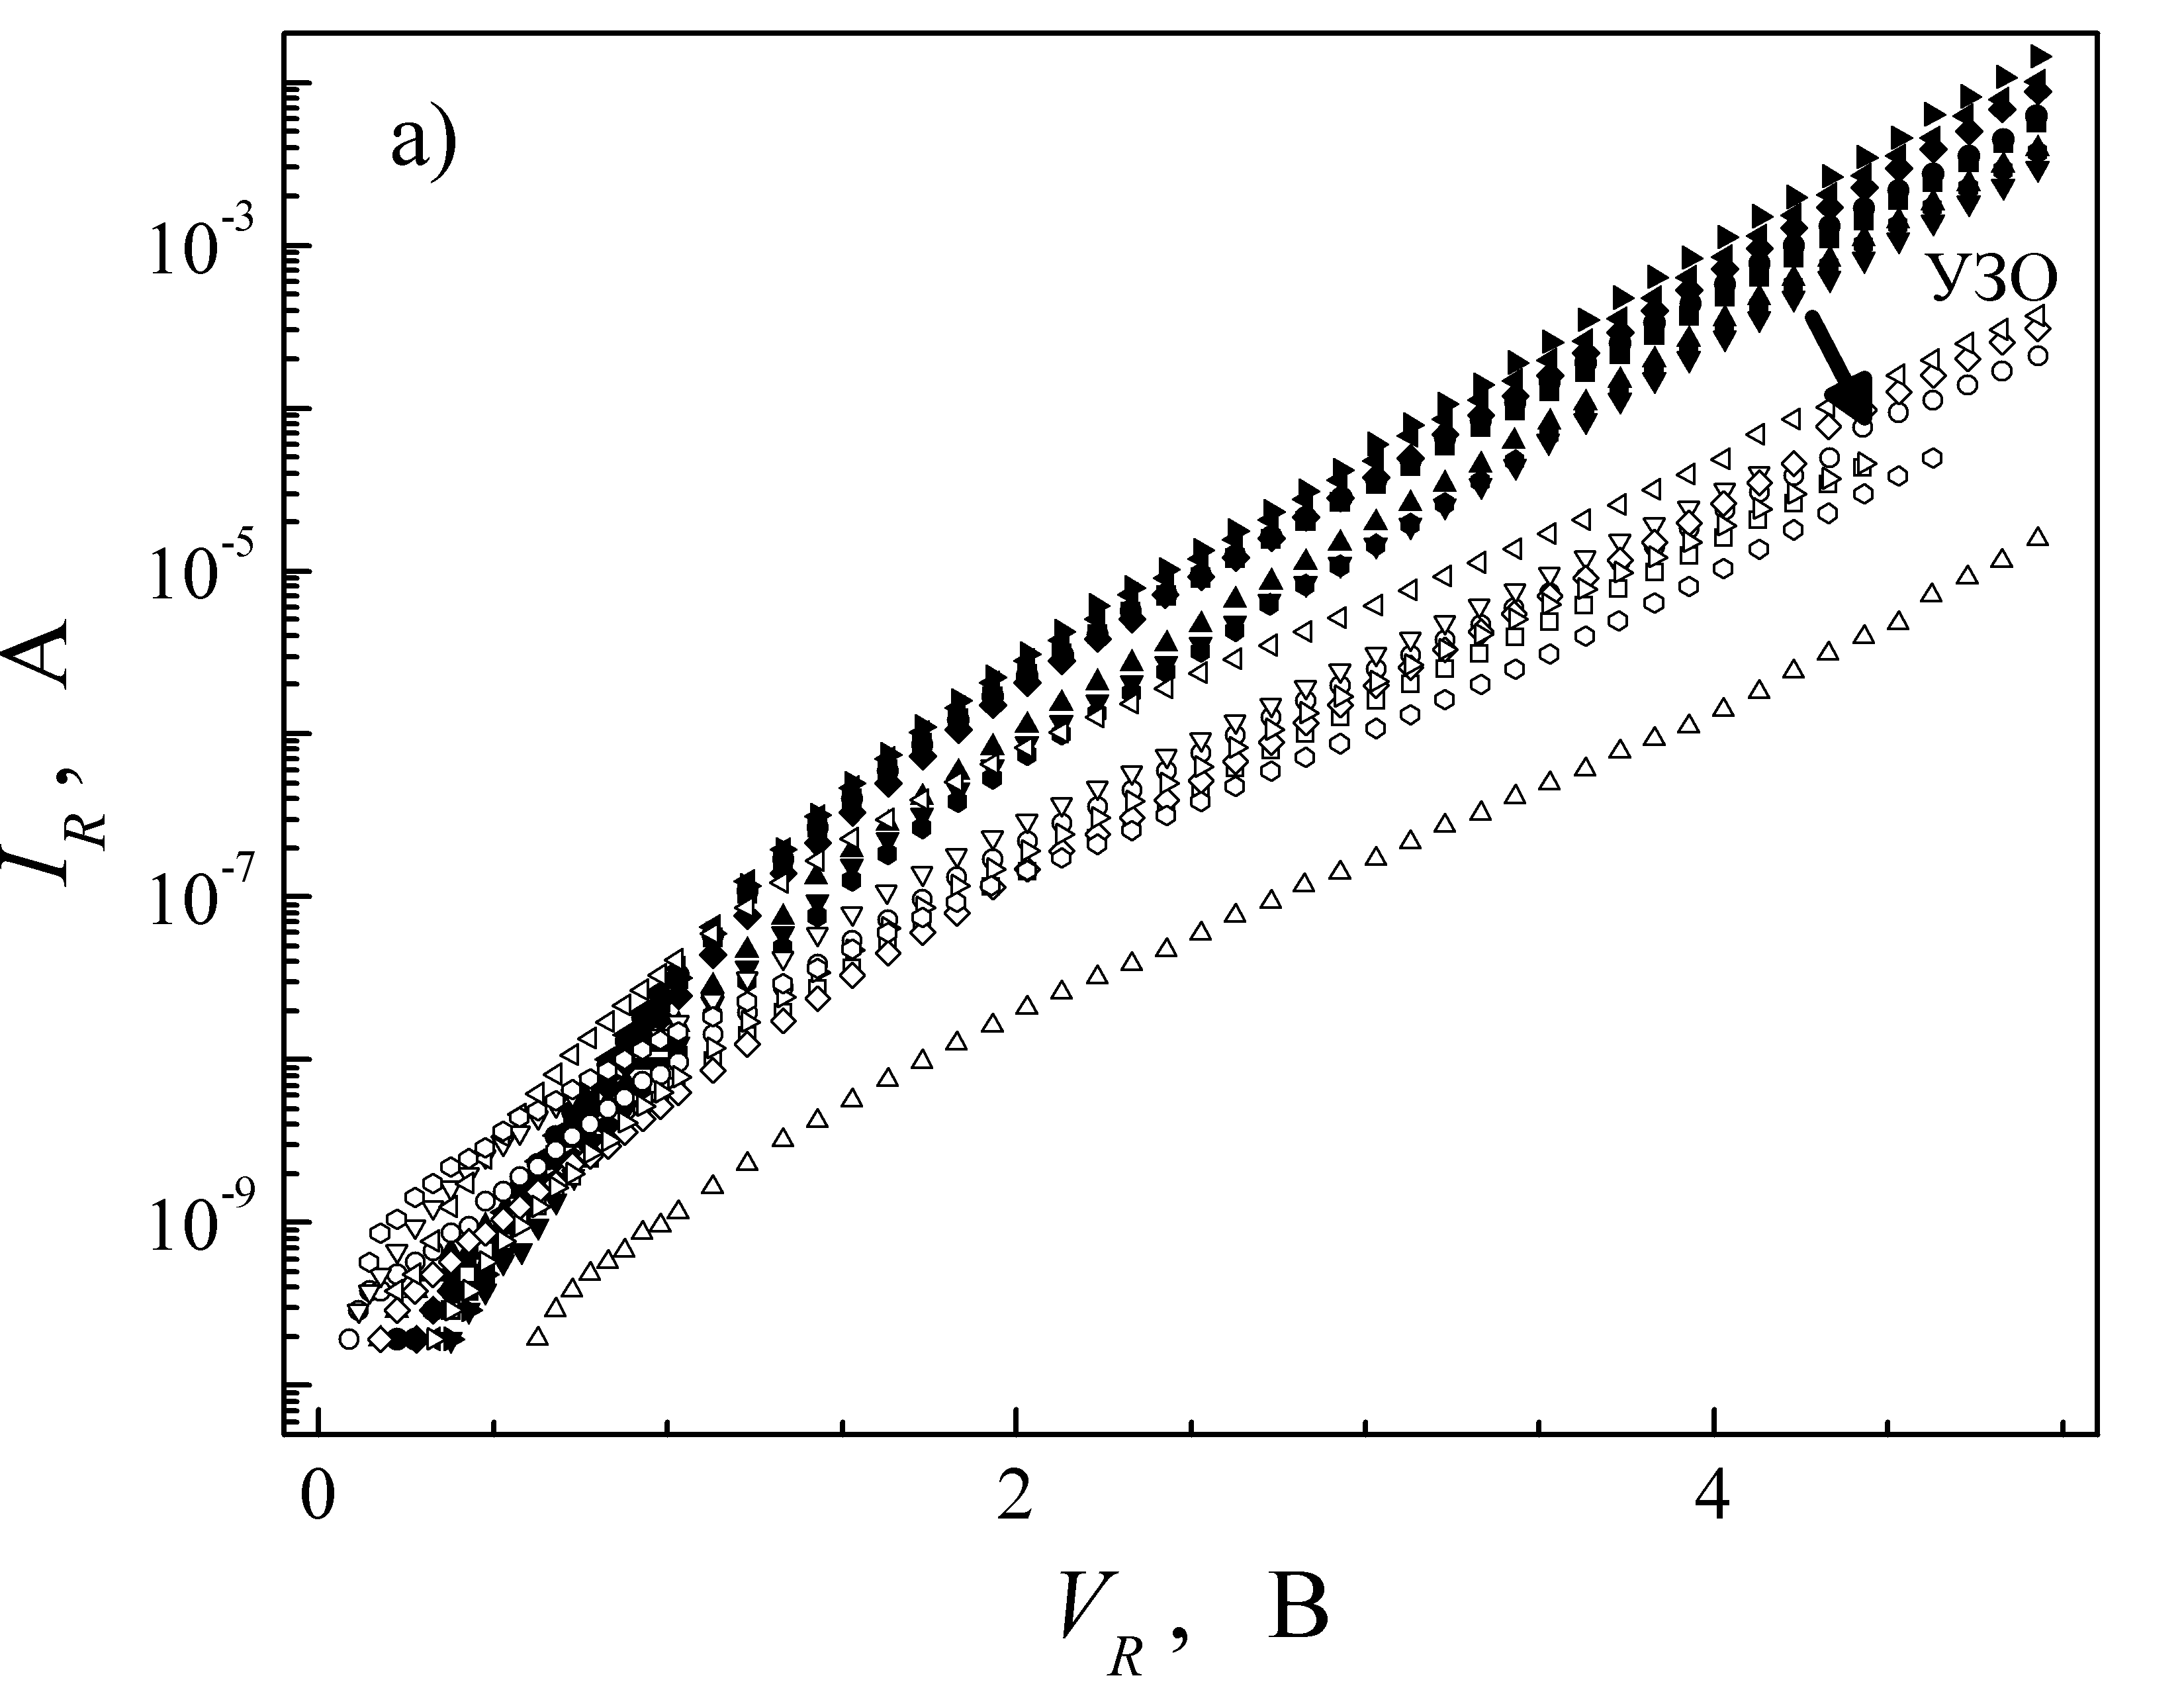
\includegraphics[width=0.49\textwidth]{figIr30_GA1} \hfill
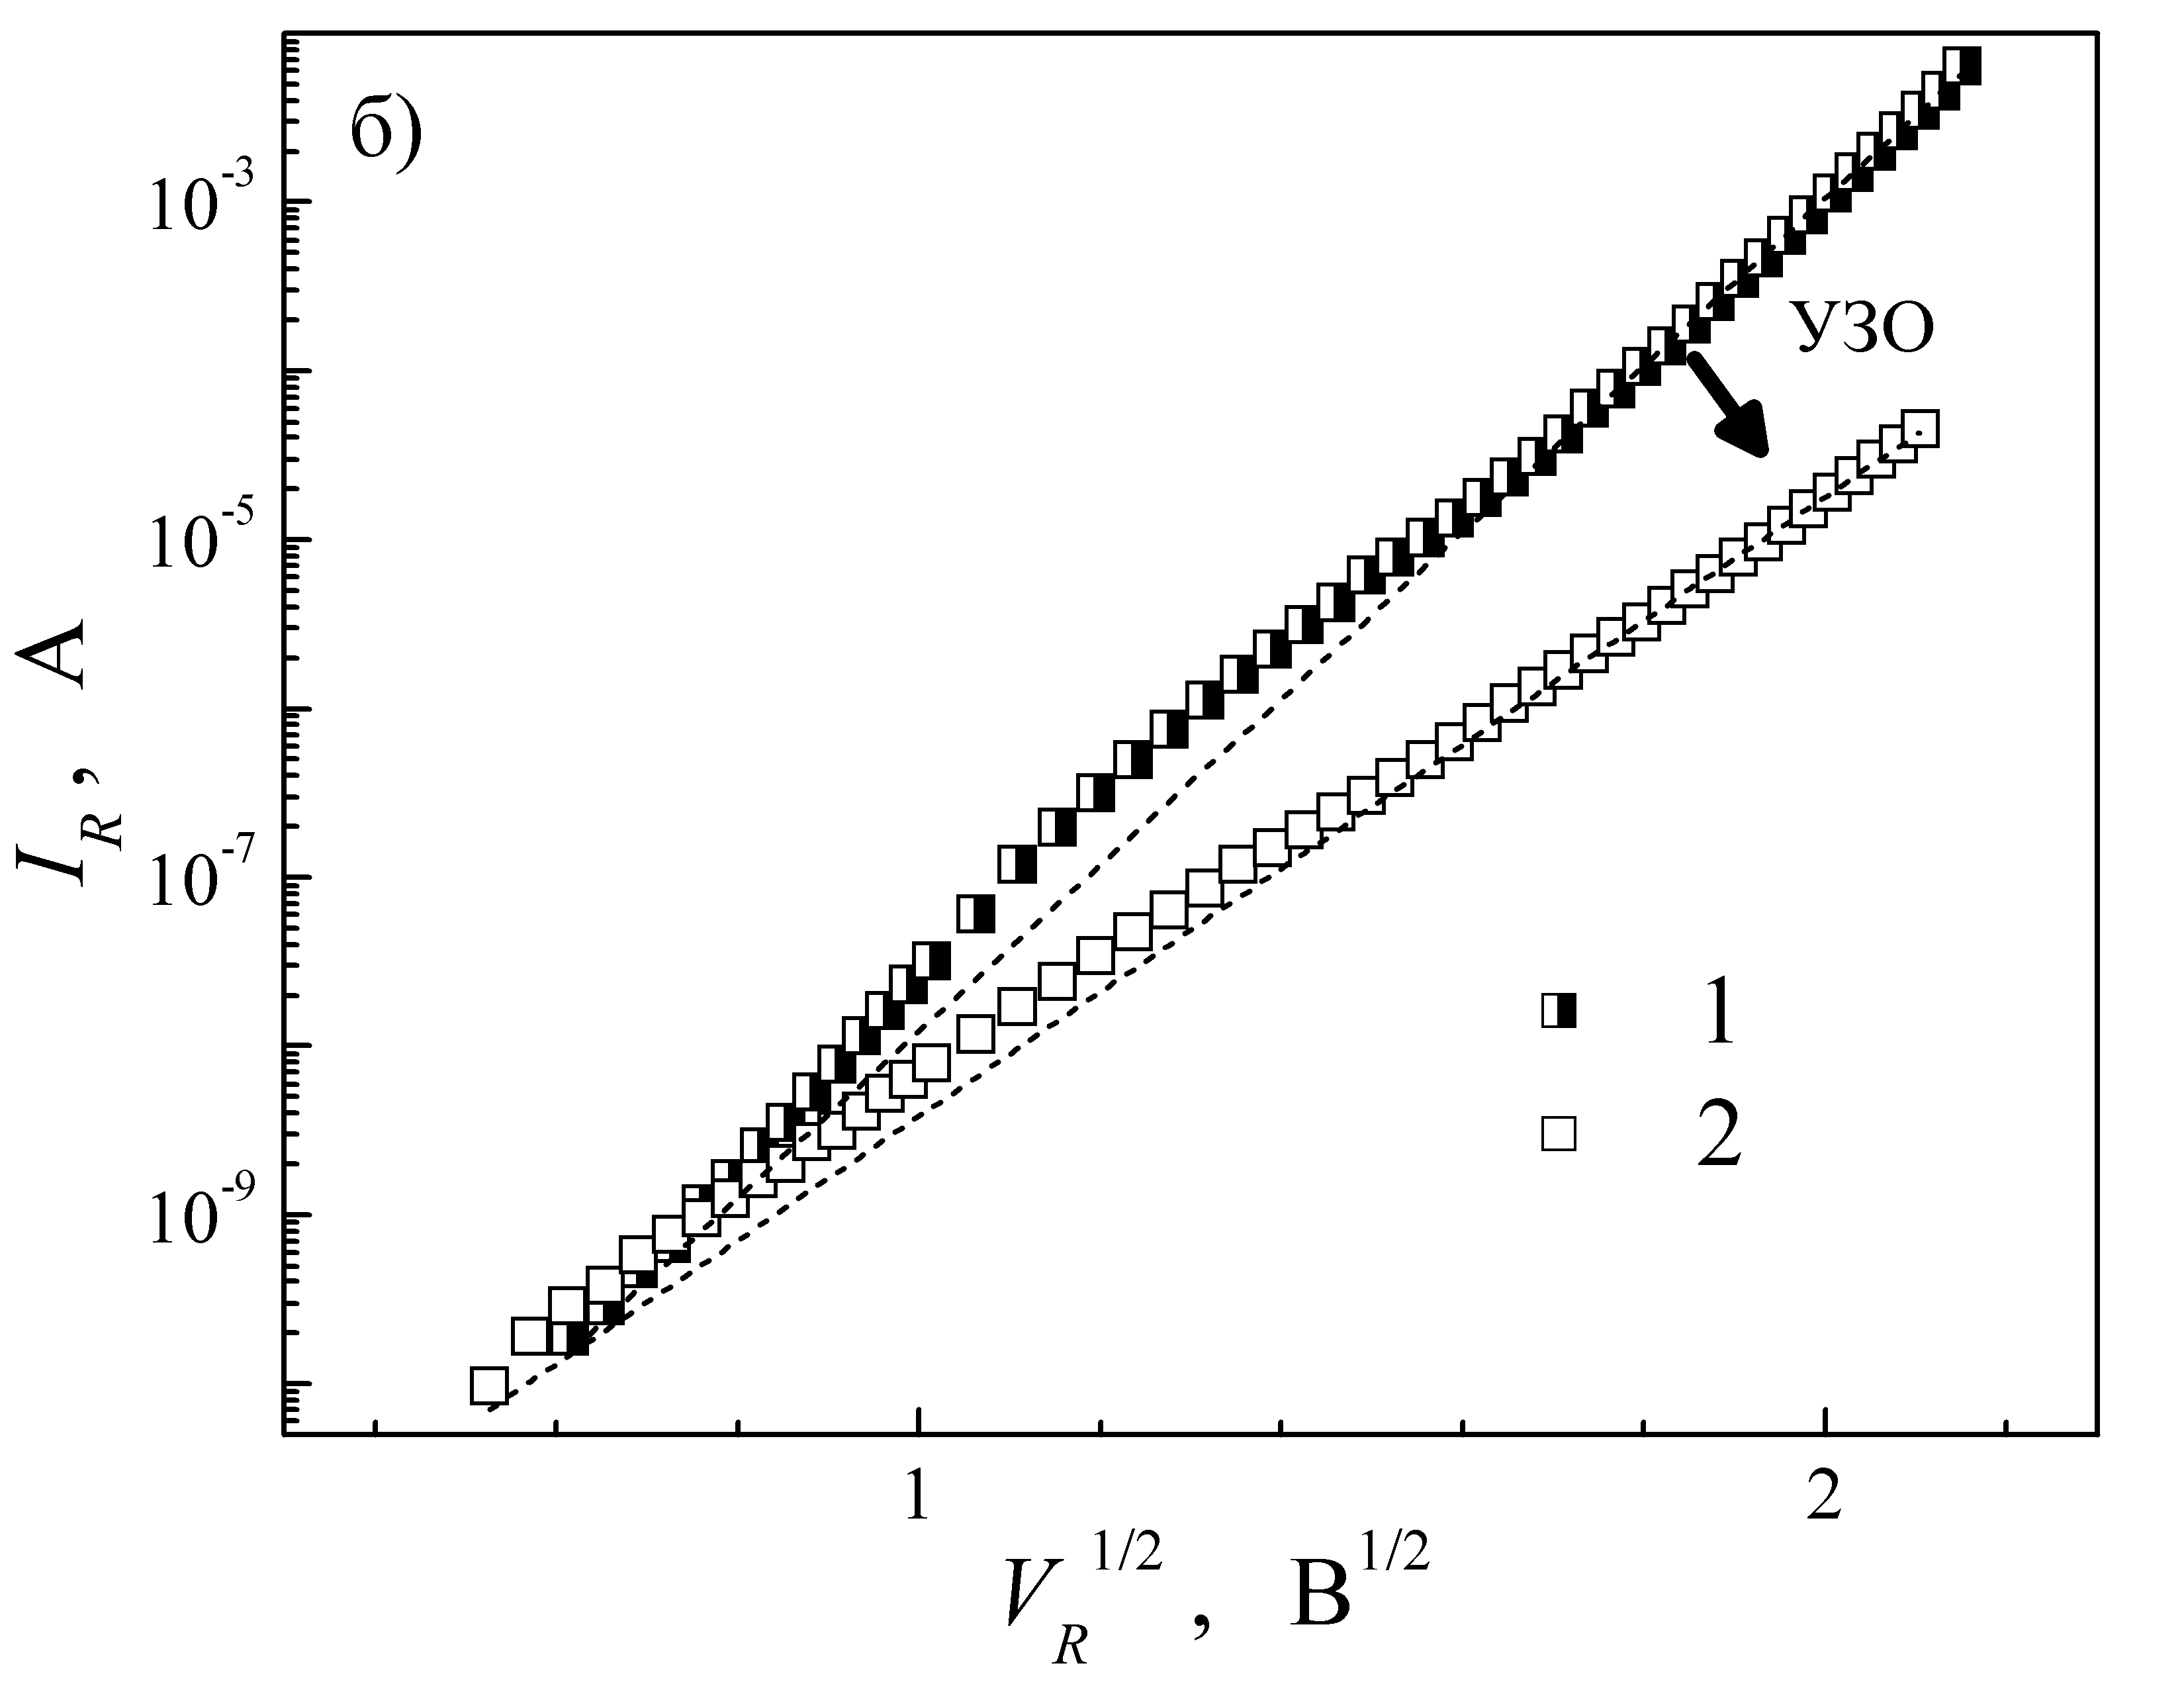
\includegraphics[width=0.49\textwidth]{figIr30_GA2}
\caption{\label{figIr30_GA}
Зворотні гілки ВАХ структур Au--TiB$_x$--$n$--$n^+$--GaAs
до УЗО (заповнені та напівзаповнені точки)
та після U30--03 (порожні точки).
Точки однакової форми відповідають однаковим діодам.
На рисунку (а) наведено криві, отримані для частини набору структур з одного зразка,
на рисунку (б) --- типові залежності для одного діоду.
Лінії --- апроксимація відповідно до (\ref{eqIR1:GA}).
$I_{s,\mathtt{tun}}$, A: $1,4\cdot10^{-13}$ (1), $8,1\cdot10^{-13}$ (2);
$a_\mathtt{tun}$, В$^{-1/2}$: 11,4 (1), 8,1 (2).
}%
\end{figure}

\begin{table}
\caption{\label{tabUS_GaAs}Характеристичний параметр тунельної компоненти
зворотного струму структур Au--TiB$_x$--$n$--$n^+$--GaAs до та після УЗО.
}
\center
\begin{tabular}{|c|c|c|}
\hline
УЗО&\multicolumn{2}{c|}{$a_\mathtt{tun}$, В$^{-1/2}$}\\ \cline{2-3}
& до УЗО & після УЗО \\
\hline
U04--18&$9,5\div11,0$&$9,5\div11,0$\\ \hline
U09--16&$9,5\div11,3$&$9,3\div10,1$\\ \hline
U30--03&$10,1\div11,3$&$8,3\div9,8$\\ \hline
\end{tabular}
\end{table}


При перевищенні інтенсивністю  УЗО порогу (як вже зазначалося раніше, близько $2,5\div3$~Вт/см$^2$) спостерігалося значне, на $1\div2$ порядки,
зростання величини зворотного струму для обох груп ДШ.
Збільшення відбулося, переважно, в наслідок внеску термоемісійної компоненти зворотного струму, зокрема для діодів першої групи в результаті високоінтенсивної УЗО
змінився характер перенесення заряду --- див Рис.~\ref{figIrWbig_GA}.
Відомо, що надпорогова УЗО здатна викликати генерацію дефектів різного типу в об’ємі та приповерхневому шарі GaAs \cite{Zaver},
спричинити перебудову дефектної структури границі розділу \cite{Parchinskii2003r}.
Для досліджених структур подібні ефекти мають викликати зниження $\Phi_b$ внаслідок ефекту Шотки та збільшення величини зворотного струму, що і спостерігається на експерименті.


\begin{figure}
\center
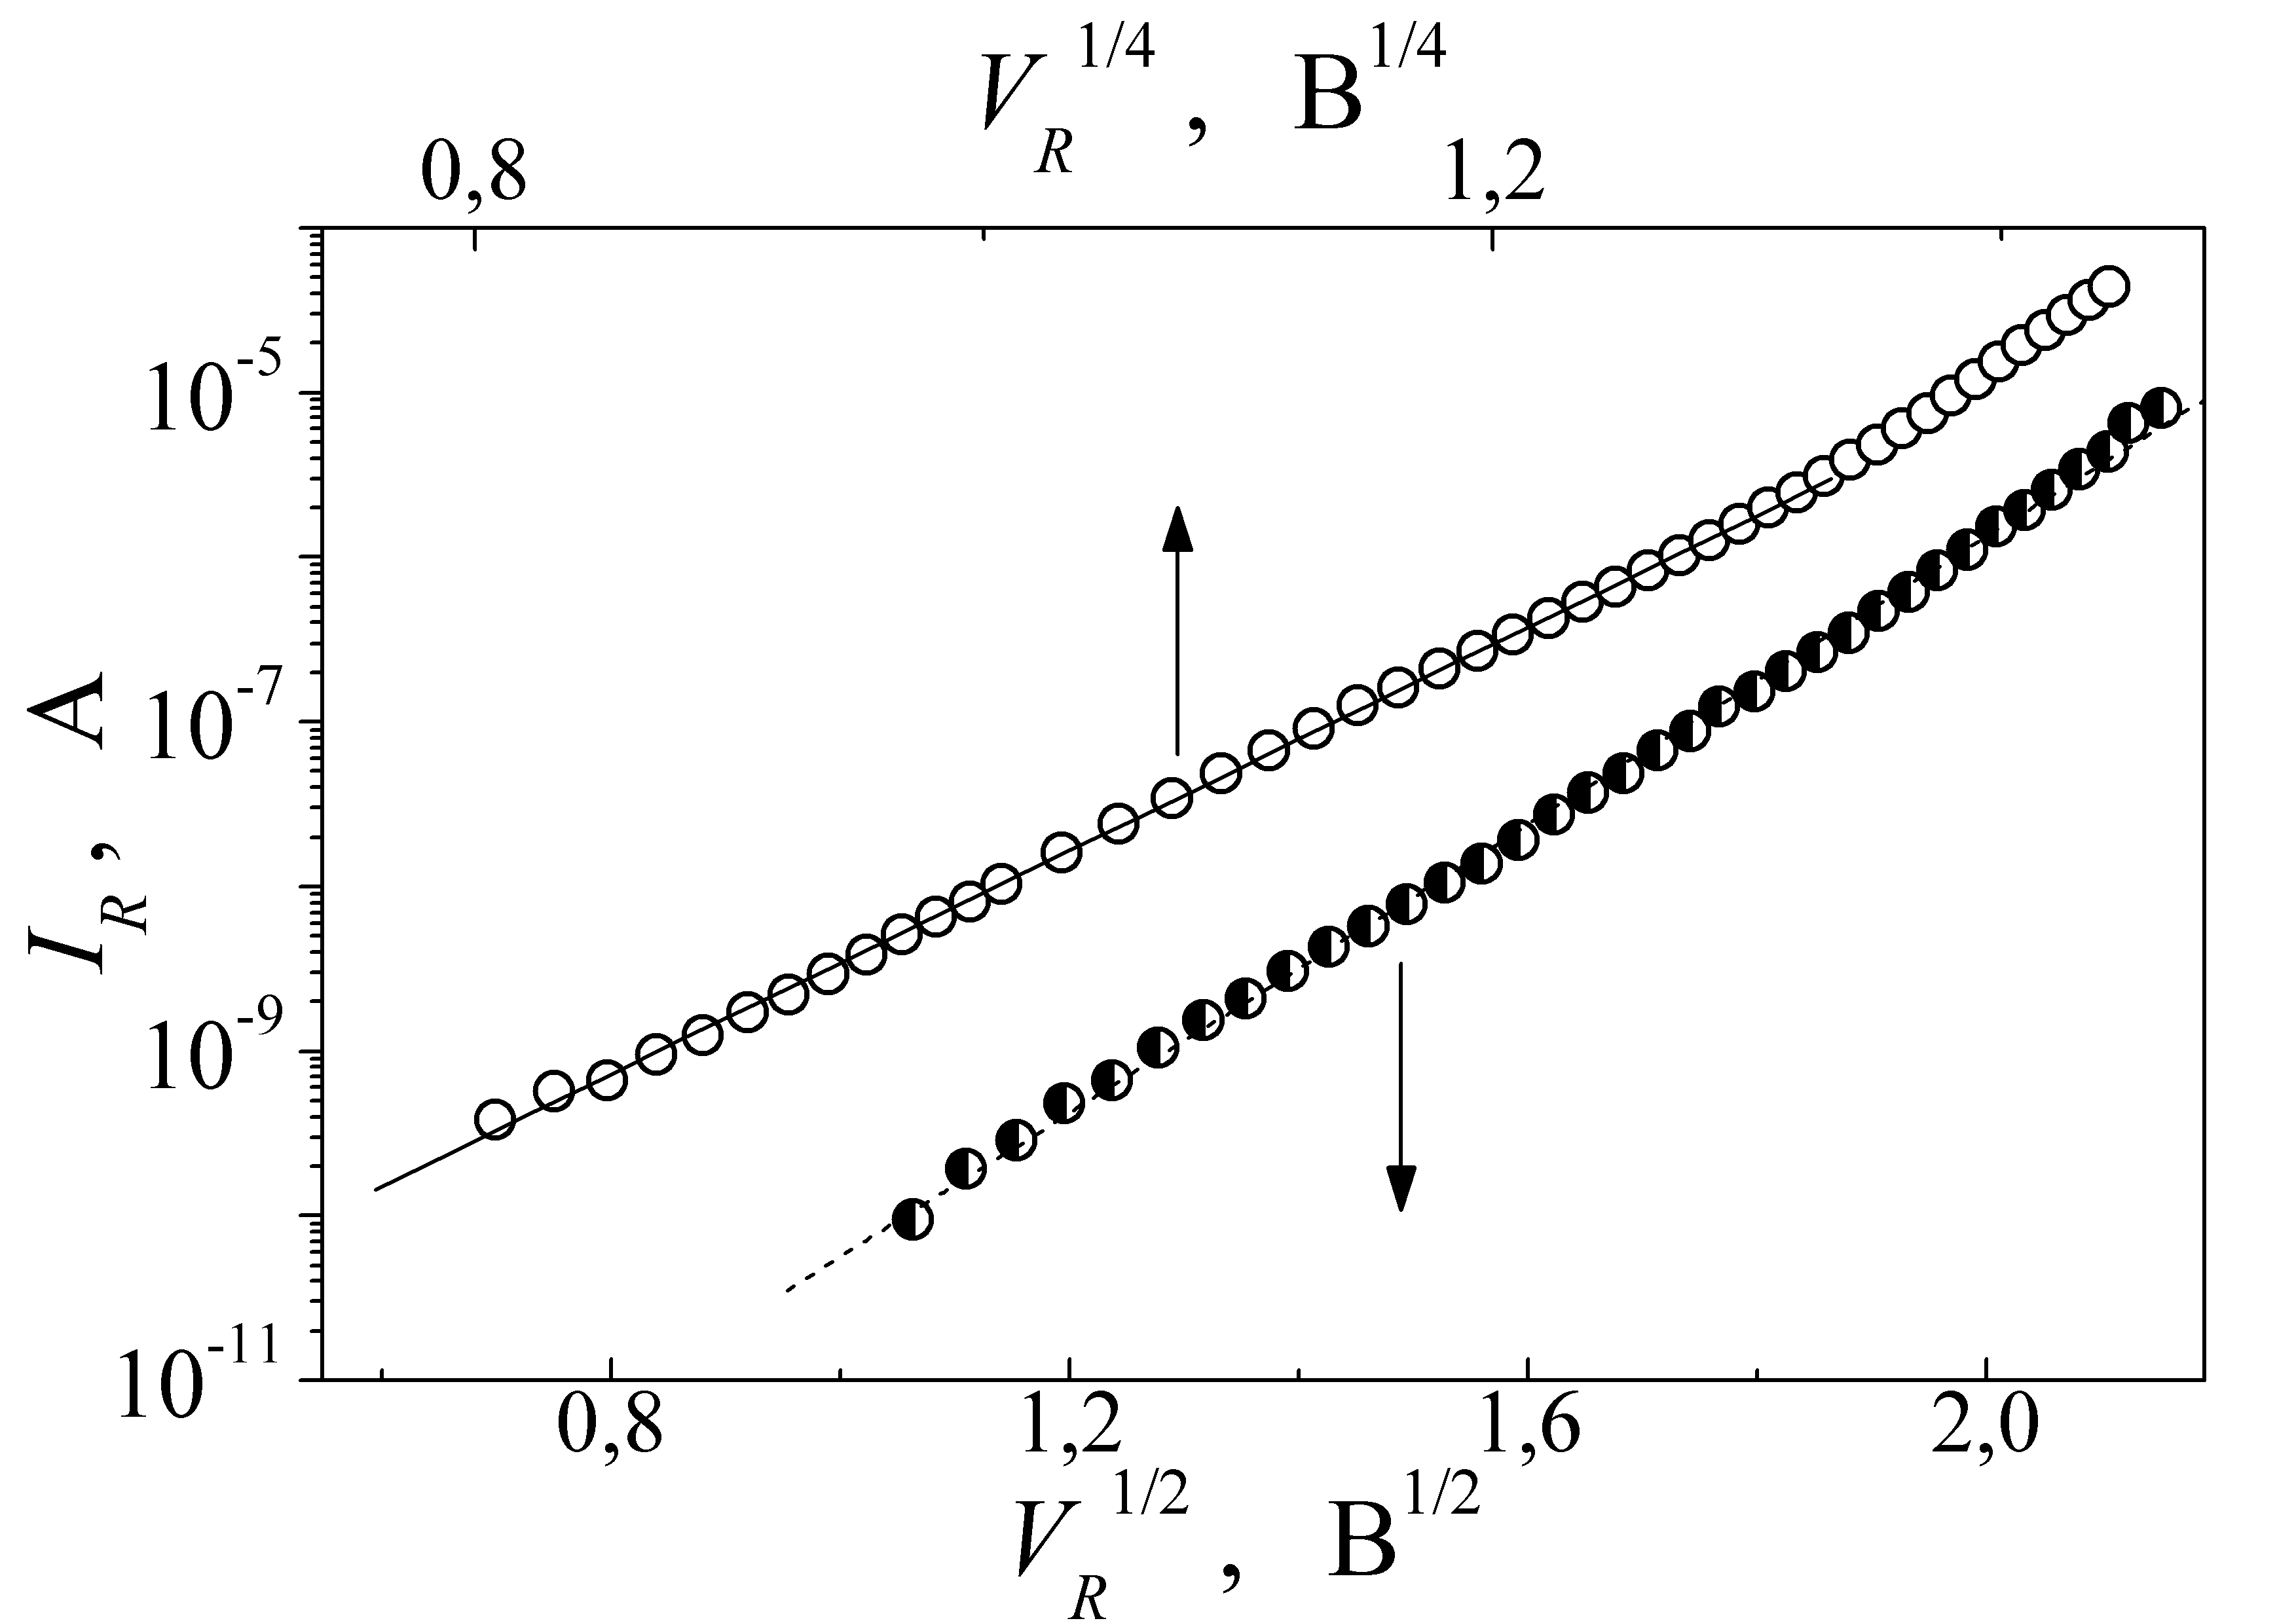
\includegraphics[width=0.65\textwidth]{figIrWbig_GA}%
\caption{\label{figIrWbig_GA}
Зворотні гілки ВАХ структури Au--TiB$_x$--$n$--$n^+$--GaAs
до УЗО (напівзаповнені точки)
та після U04--31 (порожні точки).
Точки -- експеримент,
суцільна лінія --- апроксимація частини ВАХ згідно з формулою~(\ref{eqIR2:GA}),
пунктирна  --- згідно з (\ref{eqIR1:GA}).
}%
\end{figure}




\section{Акустовідпал гамма--індукованих дефектів в структурах Si--SiO$_2$--Au}

Як вже згадувалося раніше, радіаційні дефекти, які утворюються в кристалах, можуть ефективно взаємодіяти з пружними коливаннями.
Одним з проявів цього явища є відпал дефектів в результаті УЗО при температурах, значно нижчих ніж це відбувається при без--звуковому нагріванні.
Подібні процеси спостерігалися в монокристалах кристалах кремнію \cite{OstrovRadSi,Podolian2012r,PodolHivr,YOlikh2007TPLr}, германію \cite{Olikh:FTP1996},
напівровідникових \cite{OlikhProc,OstrovFTTRad} та лужногалоїдних \cite{UST:OstrovCsI} сполук.
Як правило, подібні процеси пов'язують з розпадом радіаційноутворених комплексів під дією пружних коливань та акустоіндукованою дифузією дефектів до різноманітних стоків.
Крім того, в літературі показана можливість часткового відновлення за допомогою УЗО параметрів опромінених напівпровідникових поверхнево--бар'єрних структур, таких як, наприклад,
сонячні елементи \cite{YOlikh2007TPLr} чи світловипромінюючі діоди \cite{US:LED,UST:LED_SM}.
Найчастіше причиною появи дефектів є $\gamma$--опромінення, проте показана можливість ефективного впливу пружних коливань і на порушення періодичності, викликані
рентгенівськими променями \cite{UST:OstrovCsI}, нейтронами \cite{Olikh:FTP1996} чи електронами \cite{US:LED,UST:LED_SM}.

З іншого боку, дослідники не оминули своєю увагою і можливість впливу УЗО на властивості таких промислово--важливих структур, як система
кремній --- оксид кремнію.
Зокрема, повідомлено про АІ зміни дефектного стану границі  Si--SiO$_2$ \cite{Ostap:SiO2,UST:Medvid,Zaver:2008r} та часу життя неосновних носіїв в області кремнію,
що прилягає до контакту \cite{Parchinskii2003r,Zdeb1989}.
Крім того, декілька робіт присвячено виявленню наслідків УЗО структур метал--окис--напівпровідник (МОН) на основі кремнію, опромінених $\gamma$--квантами $^{60}$Co \cite{Parchinskii2000r,Parchinskii2006r}.
Об'єктом досліджень авторів даних робіт були структури Si--SiO$_2$ виготовлені методом термічного окислення пластин кремнію $n$--типу з питомим опором 0,2~Ом$\cdot$см.
Поглинута доза опромінення складала $10^6$~рад.
В результаті вимірів ВФХ було зроблено висновок про зменшення ефективного поверхневого заряду та генераційного часу життя в приконтактній області кремнію та незначне
зростання швидкості поверхневої рекомбінації.
Автори пов'язують виявлені ефекти з дифузією дефектів та розпадом домішкових асоціатів в акустичному полі, причому зазначають , що виявлені процеси
послаблені, порівняно з неопроміненими структурами, внаслідок радіаційностимульваної релаксації напруг в області границі Si--SiO$_2$.

У цьому параграфі представлені результати досліджень впливу УЗО на процеси перенесення заряду в радіаційноопромінених структурах Si--SiO$_2$--Au.
Метою роботи було з'ясування можливості відновлення працездатності діодів Шотки, створених на основі МОН структур і суттєво деградованих внаслідок опромінення.
Хоча вищезазначені роботи \cite{Parchinskii2000r,Parchinskii2006r} і були певними експериментальними передумовами для проведення наших досліджень, проте
підкреслимо що суттєві відмінності представлених результатів полягають у тому, що вони отримані
а)~для систем зі значно вищою концентрацією радіаційних дефектів;
б)~при розгляді робочого режиму ДШ, тобто при проходженні струму.



Зразки для досліджень були виготовлені з кристалічного кремнію, вирощеного методом зонної плавки.
Для легування використовувалися атоми фосфору, питомий опір кристалів складав 4000~Ом$\cdot$см.
З об'ємного матеріалу було вирізано зразки у формі паралелепіпеда розмірами $1\times5\times10$~мм$^3$.
Для формування структури МОН одна з поверхонь площею 50~мм$^2$ хімічно очищувалася в розчині HF--HNO$_3$--CH$_3$COOH (об'ємне співвідношення компонент 3:5:3),
після чого в атмосферному повітрі при $T=300$~К протягом 24~год на ній формувався шар SiO$_2$.
Надалі шляхом вакуумного напилення на поверхню наносився шар золота (30~мкг/cm$^2$).
На протилежній грані за допомогою евтектики GaZn створювався омічний контакт.
Схематичне зображення структури зразків показано на Рис.~\ref{figMSSi3}.

\begin{figure}[b]
\center
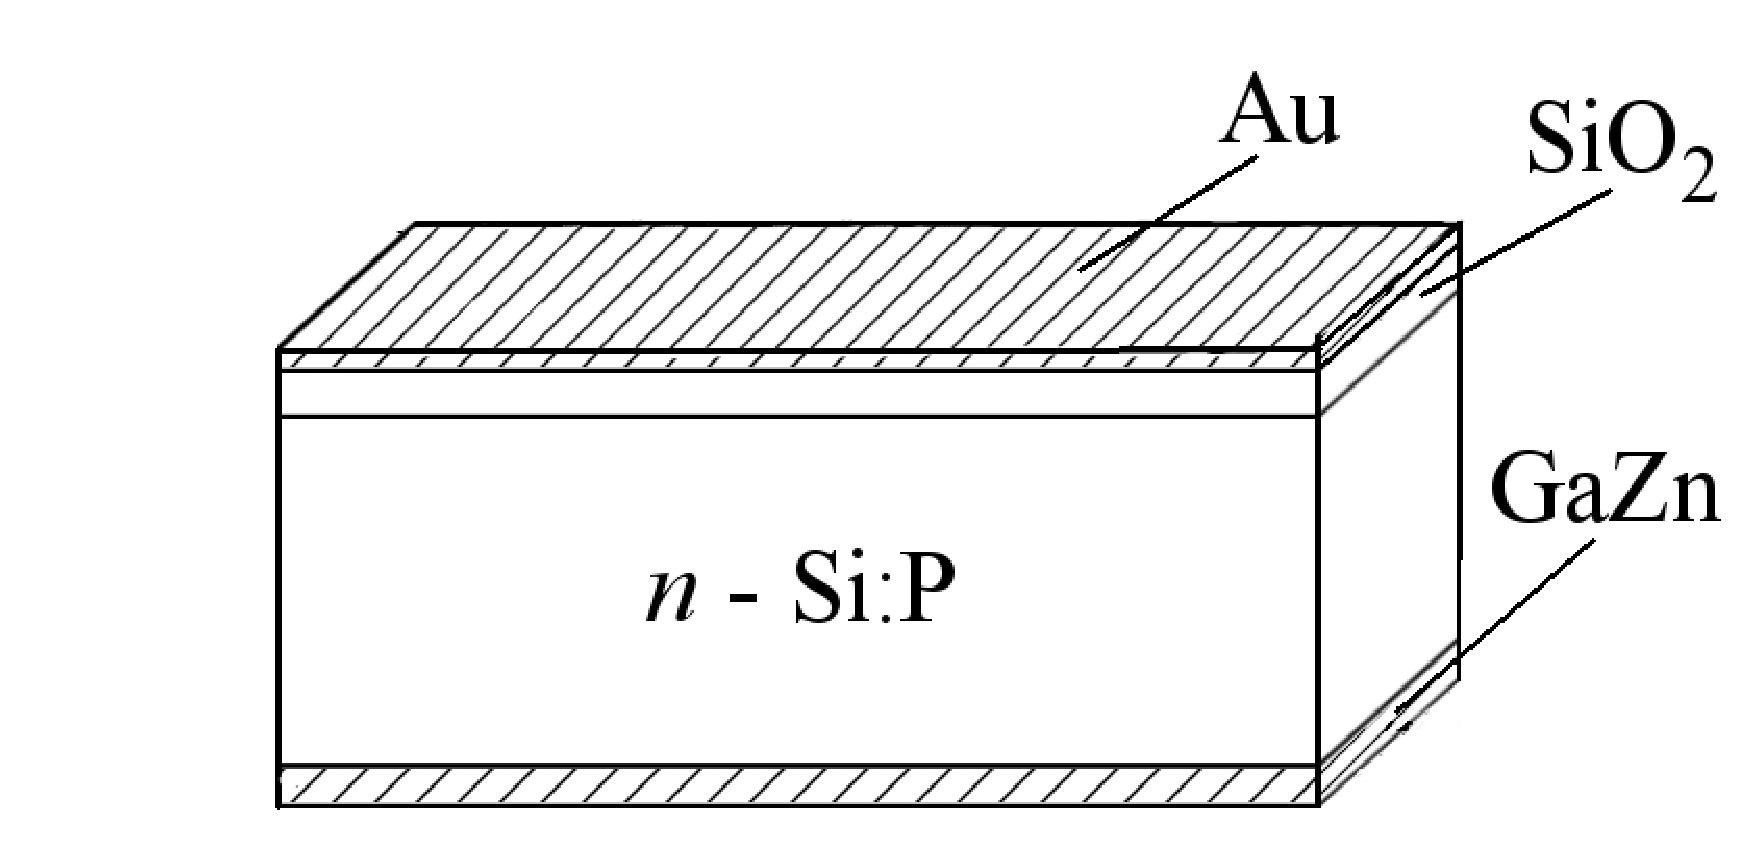
\includegraphics[width=0.6\textwidth]{MSSi3}%
\caption{\label{figMSSi3}
Структура зразків Si--SiO$_2$--Au.
}
\end{figure}

Опромінення здійснювалось при кімнатній температурі $\gamma$--квантами $^{60}$Co, доза дорівнювала $5\cdot10^7$~рад.
Як показали вимірювання, після еквівалентного опромінення провідність монокристалічних зразків за величиною зменшилась приблизно в 2 рази залишаючись електронною за типом,
що пов'язано з частковою компенсацією в процесі радіаційного дефектоутворення.
Зауважимо, що питомий опір досліджених кристалів на чотири порядки більший, ніж в роботах \cite{Parchinskii2000r,Parchinskii2006r}, а отже частка енергетичних втрат, не пов'язанихз іонізацією, для гамма-квантів в нашому випадку значно вища.
Доза також на півтора порядку вища, і тому очікувана концентрація радіаційних дефектів суттєво вища.


УЗО опромінених структур інтенсивністю 2~Вт/см$^2$ здійснювалась за допомогою LiNbO$3$ п'єзоелектричного перетворювача.
У зразку збуджувалися повздовжні хвилі частотою 4~МГц.
Було проведено дві послідовні УЗО, кожна тривалістю 30~хв.
Під час УЗО температура зразка не перевищувала 350~К.

На Рис.~\ref{figIV_MIS} наведено ВАХ структур  Si--SiO$_2$--Au до $\gamma$--опромінення, після нього та після наступних УЗО.
З рисунка видно, що у вихідному стані ВАХ є типовою для ДШ:
при прямому зміщенні струм пов'язаний ТЕ через бар'єр,
при зворотному --- величина струму визначається зміною висоти бар'єру під дією електричного поля ($I_R\sim V_R^{1/2}$).
Для апроксимації прямої гілки ВАХ був використаний вираз (\ref{eqSDIV});
результат апроксимації показано на Рис.~\ref{figIV_MIS},а та б, визначені параметри
наведені в Таблиці~~\ref{tabMIS}.
Зауважимо, що наявність шару оксиду не дозволяє визначити ВБШ безпосередньо використовуючи величину струму насичення та формулу~(\ref{eqSDIs}), так як необхідно також враховувати ймовірність проходження через діелектричний прошарок \cite{OZBEK2011,Kobayashi}.
Крім того, як видно з рисунку, при $V>1$~В в неопромінених структурах величина струму перевищує значення, очікуване відповідно до виразу (\ref{eqSDIV}).
На нашу думку, це пов'язане з тунелюванням через шар SiO$_2$, яке, загалом, може бути описане виразом \ref{eqFowlNord}.
На користь цього припущення свідчить лінійність польової залежності величини прямого струму в координатах Фаулера--Нордгейма при великих прямих зміщеннях --- див. вставку на Рис.~\ref{figIV_MIS}.
При побудові цієї залежності враховано, що величина електричного поля в прошарку оксиду товщиною $d_{ox}$ пропорційна прикладеній напрузі $F_m\sim V/d_{ox}$.

\begin{figure}
\center
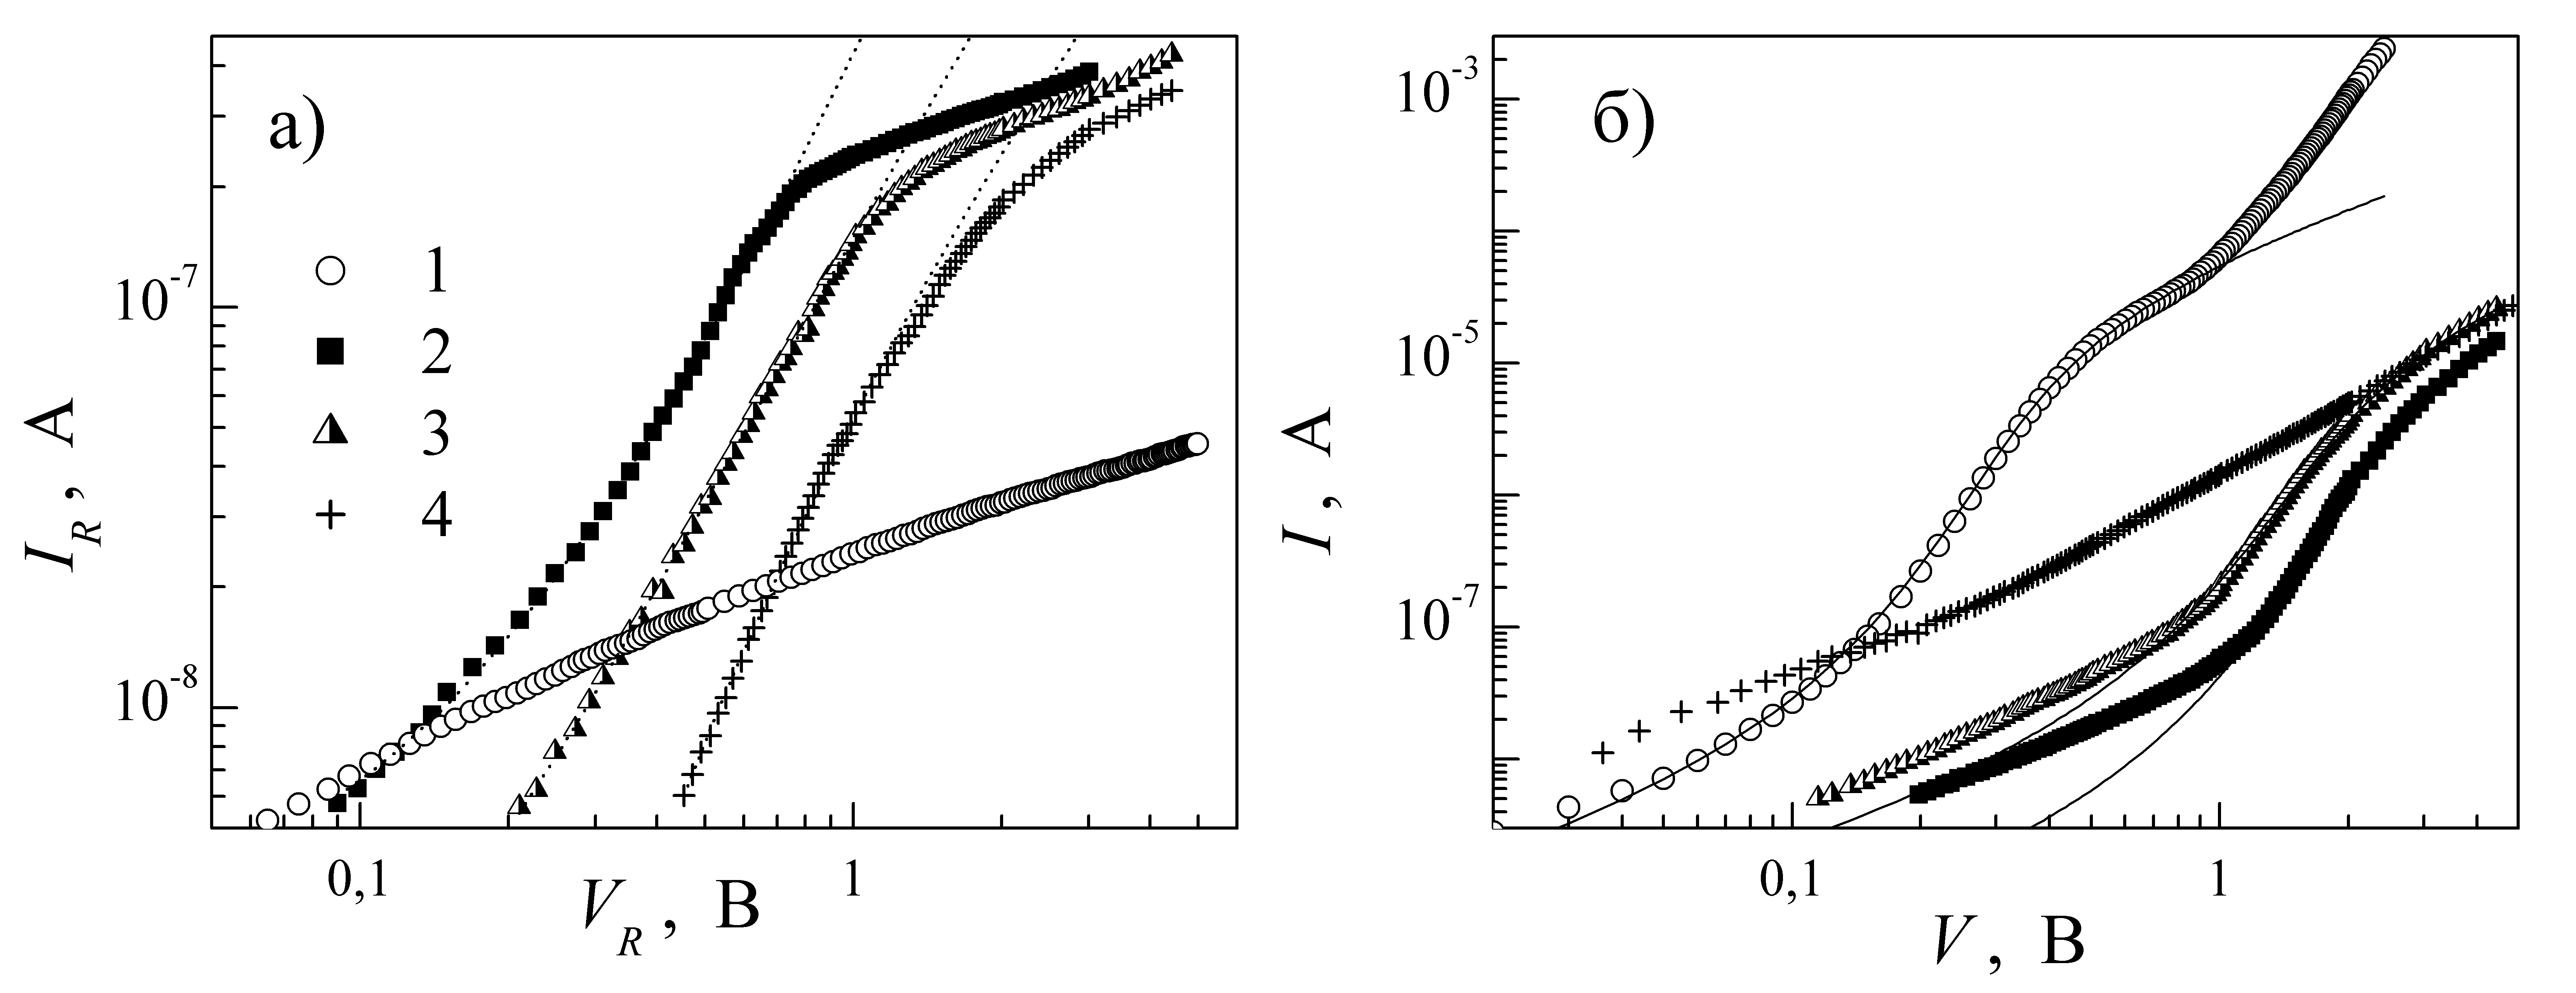
\includegraphics[width=0.95\textwidth]{figIV_MIS}%
\caption{\label{figIV_MIS}
Прямі (а, в) та зворотні (а, б) ВАХ структур Si--SiO$_2$--Au до (криві 1)
та після (2--4) опромінення $\gamma$--квантами в напівлогарифмічному (а)
та подвійному логарифмічному (б, в) масштабах.
$t_\mathtt{UST}$ , хв: 0 (2), 30 (3), 60 (4).
$T=300$~K.
Точки --- експеримент,
лінії --- апроксимація за формулами~(\ref{eqSDIV}) (суцільні) та (\ref{eqIVTAT}) (пунктир).
Параметри апроксимацій вказані в Таблиці~\ref{tabMIS}.
На вставці:
залежність прямої компоненти струму неопроміненого зразка (при $V>1.6$~В) в координатах Фаулера--Нордгейма;
пряма --- лінійна апроксимація.
}%
\end{figure}





Внаслідок $\gamma$--опромінення характер проходження струму суттєво змінився --- див. криві 2 на Рис.~\ref{figIV_MIS}.
Особливо це стосується зворотної гілки ВАХ (Рис.~\ref{figIV_MIS},б), де кардинальні видозміни польової залежності струму свідчать про зміну механізму перенесення заряду.
При прямому зміщенні залежність $I(V)$, очікувана в рамках ТЕ моделі, спостерігається лише при напрузі, більшій 1~В (Рис.~\ref{figIV_MIS},в), а величина струму суттєво менша, ніж до опромінення.
Як показала апроксимація відповідної ділянки ВАХ згідно з формулою~(\ref{eqSDIV}), в результаті опромінення відбулося значне  зростання фактору неідеальності та послідовного опору (причому зміни останнього суттєво перевищують зміни питомого опору, які спостерігаються в об'ємних зразках).
Радіаційноіндуковане збільшення $n_\mathrm{id}$, пов'язане з утворенням дефектів, і є головною причиною зменшення величини термоемісійного струму.
В роботі \cite{FZSi:Rad} проведено дослідження процесів дефектоутворення в кремнії, метод вирощування і питомий опір якого співпадають з дослідженими структурами, в результаті опромінення $\gamma$--квантами $^{60}$Co з дозою близько $9\cdot10^7$~рад.
Авторами  показано, що основними радіаційними дефектами в цьому випадку є комплекси VO$_i$, С$_i$C$_s$, $Н$--центр (V$_2$O$_i$), $\Gamma$--центр та міжвузольний дефект $I^{0/-}$.
Останній є вторинним дефектом і саме з ним пов'язуються процеси компенсації (інверсії) провідності.


\begin{table}
\caption{\label{tabMIS}Параметри структур Si--SiO$_2$--Au, визначені з ВАХ.
}
\center
\begin{tabular}{|l|c|c|c|c|}
\hline
\multicolumn{5}{|c|}{Стан структури}\\\hline
$\gamma$--опромінення&$-$&$+$&$+$&$+$\\ \hline
$t_\mathtt{UST}$ , хв&0&0&30&60\\ \hline
\multicolumn{5}{|c|}{Параметр}\\\hline
$I_s$, $10^{-9}$A & 3,3& 1,1& 4,9& \\ \hline
$R_s$, $10^{4}$Ом & 1,1& 13& 8,8& \\ \hline
$n_\mathrm{id}$ & 1,7& 10,3& 9,9& \\ \hline
$m_\mathrm{F}$ & &1,3& 1,6& 1,8 \\ \hline
$I_0$ & &$4,5\cdot10^{-8}$& $1,3\cdot10^{-7}$& $1,5\cdot10^{-6}$ \\ \hline
$I_{0,\mathrm{TAT}}$, відн.од. & &1& 0,14& 0,04 \\ \hline
$U_d$, B & &0,73& 0,44& 0,12 \\ \hline
$R_\mathrm{TAT}$, відн.од. & &1& 0,54& 0,33 \\ \hline
$K_\mathrm{RECT}$ ($V=0,5$~V)&770 &0,22& 1,33& 5,4 \\ \hline
\end{tabular}
\end{table}


Зростання послідовного опору (приблизно на порядок) призвело до зменшення частки падіння напруги на діелектричному прошарку.
Як наслідок, напруження електричного поля перестало бути достатнім для ефективного тунелювання Фаулера--Нордгейма і відповідна компонента струму перестала спостерігатися.

При малих зміщеннях ($V<1$~В), як видно з Рис.~\ref{figIV_MIS},в, пряма ВАХ опромінених структур добре описується показниковою залежністю
\begin{equation}\label{eqVIsclc}
  I=I_0\,V^{\,m_\mathrm{F}},
\end{equation}
де диференційний показник ступеня $m_\mathrm{F}$ може бути визначений використовуючи співвідношення
\begin{equation}\label{eqmsclc}
  m_\mathrm{F}=\frac{V}{I}\frac{\partial V}{\partial I}.
\end{equation}
Залежність (\ref{eqVIsclc}) характерна для проходження струму обмеженого просторовим зарядом \cite{SCLC:MA2016,Jafar,SCLC:Kaya}, при цьому величина $m_\mathrm{F}$ відображає енергетичний розподіл пасток, які емітують носії струму.
Для структур після $\gamma$--опромінення і перед УЗО $m_\mathrm{F}\approx1,3$, що свідчить про експоненційний розподіл рівнів пасток по енергії.
Як відомо \cite{SCLC:MA2016,Jafar,SCLC:Kaya}, в цьому випадку $I_0$ залежить від загальної концентрації пасток $N_t$
\begin{equation}\label{eqIoSCLC}
  I_0\sim N_t^{1-m_\mathrm{F}},
\end{equation}
а температурна залежність показника ступеня описується виразом
\begin{equation}\label{eqMT_IoSCLC}
  m_\mathrm{F}=1+\frac{T_c}{T},
\end{equation}
де
$T_c$ --- характеризує розподіл пасток по енергії:
концентрація рівнів на одиницю енергії $E$ пропорційна $\exp(-E/kT_c)$.

Вираз, що описує струм у SCLC--режимі також часто записують у вигляді \cite{Jafar}:
\begin{equation}\label{eqVIsclcT}
  I(V,T)=C\exp\left(-\frac{E_x}{kT}\right)\,V^{\,m_\mathrm{F}(T)},
\end{equation}
де
$C$ --- певна константа,
$E_x$ --- енергія активації, що визначається положенням заповнених пасток стосовно зони провідності.
На Рис.~\ref{figEa_MIS} представлена температурна залежність прямого струму при $V=0,4$~В, скорегована з врахуванням
температурної залежності показника ступеня (\ref{eqMT_IoSCLC}).
Видно, що вона дійсно добре описується виразом (\ref{eqVIsclcT}), причому $E_x=(0,32\pm0,01)$~еВ.

\begin{figure}
\center
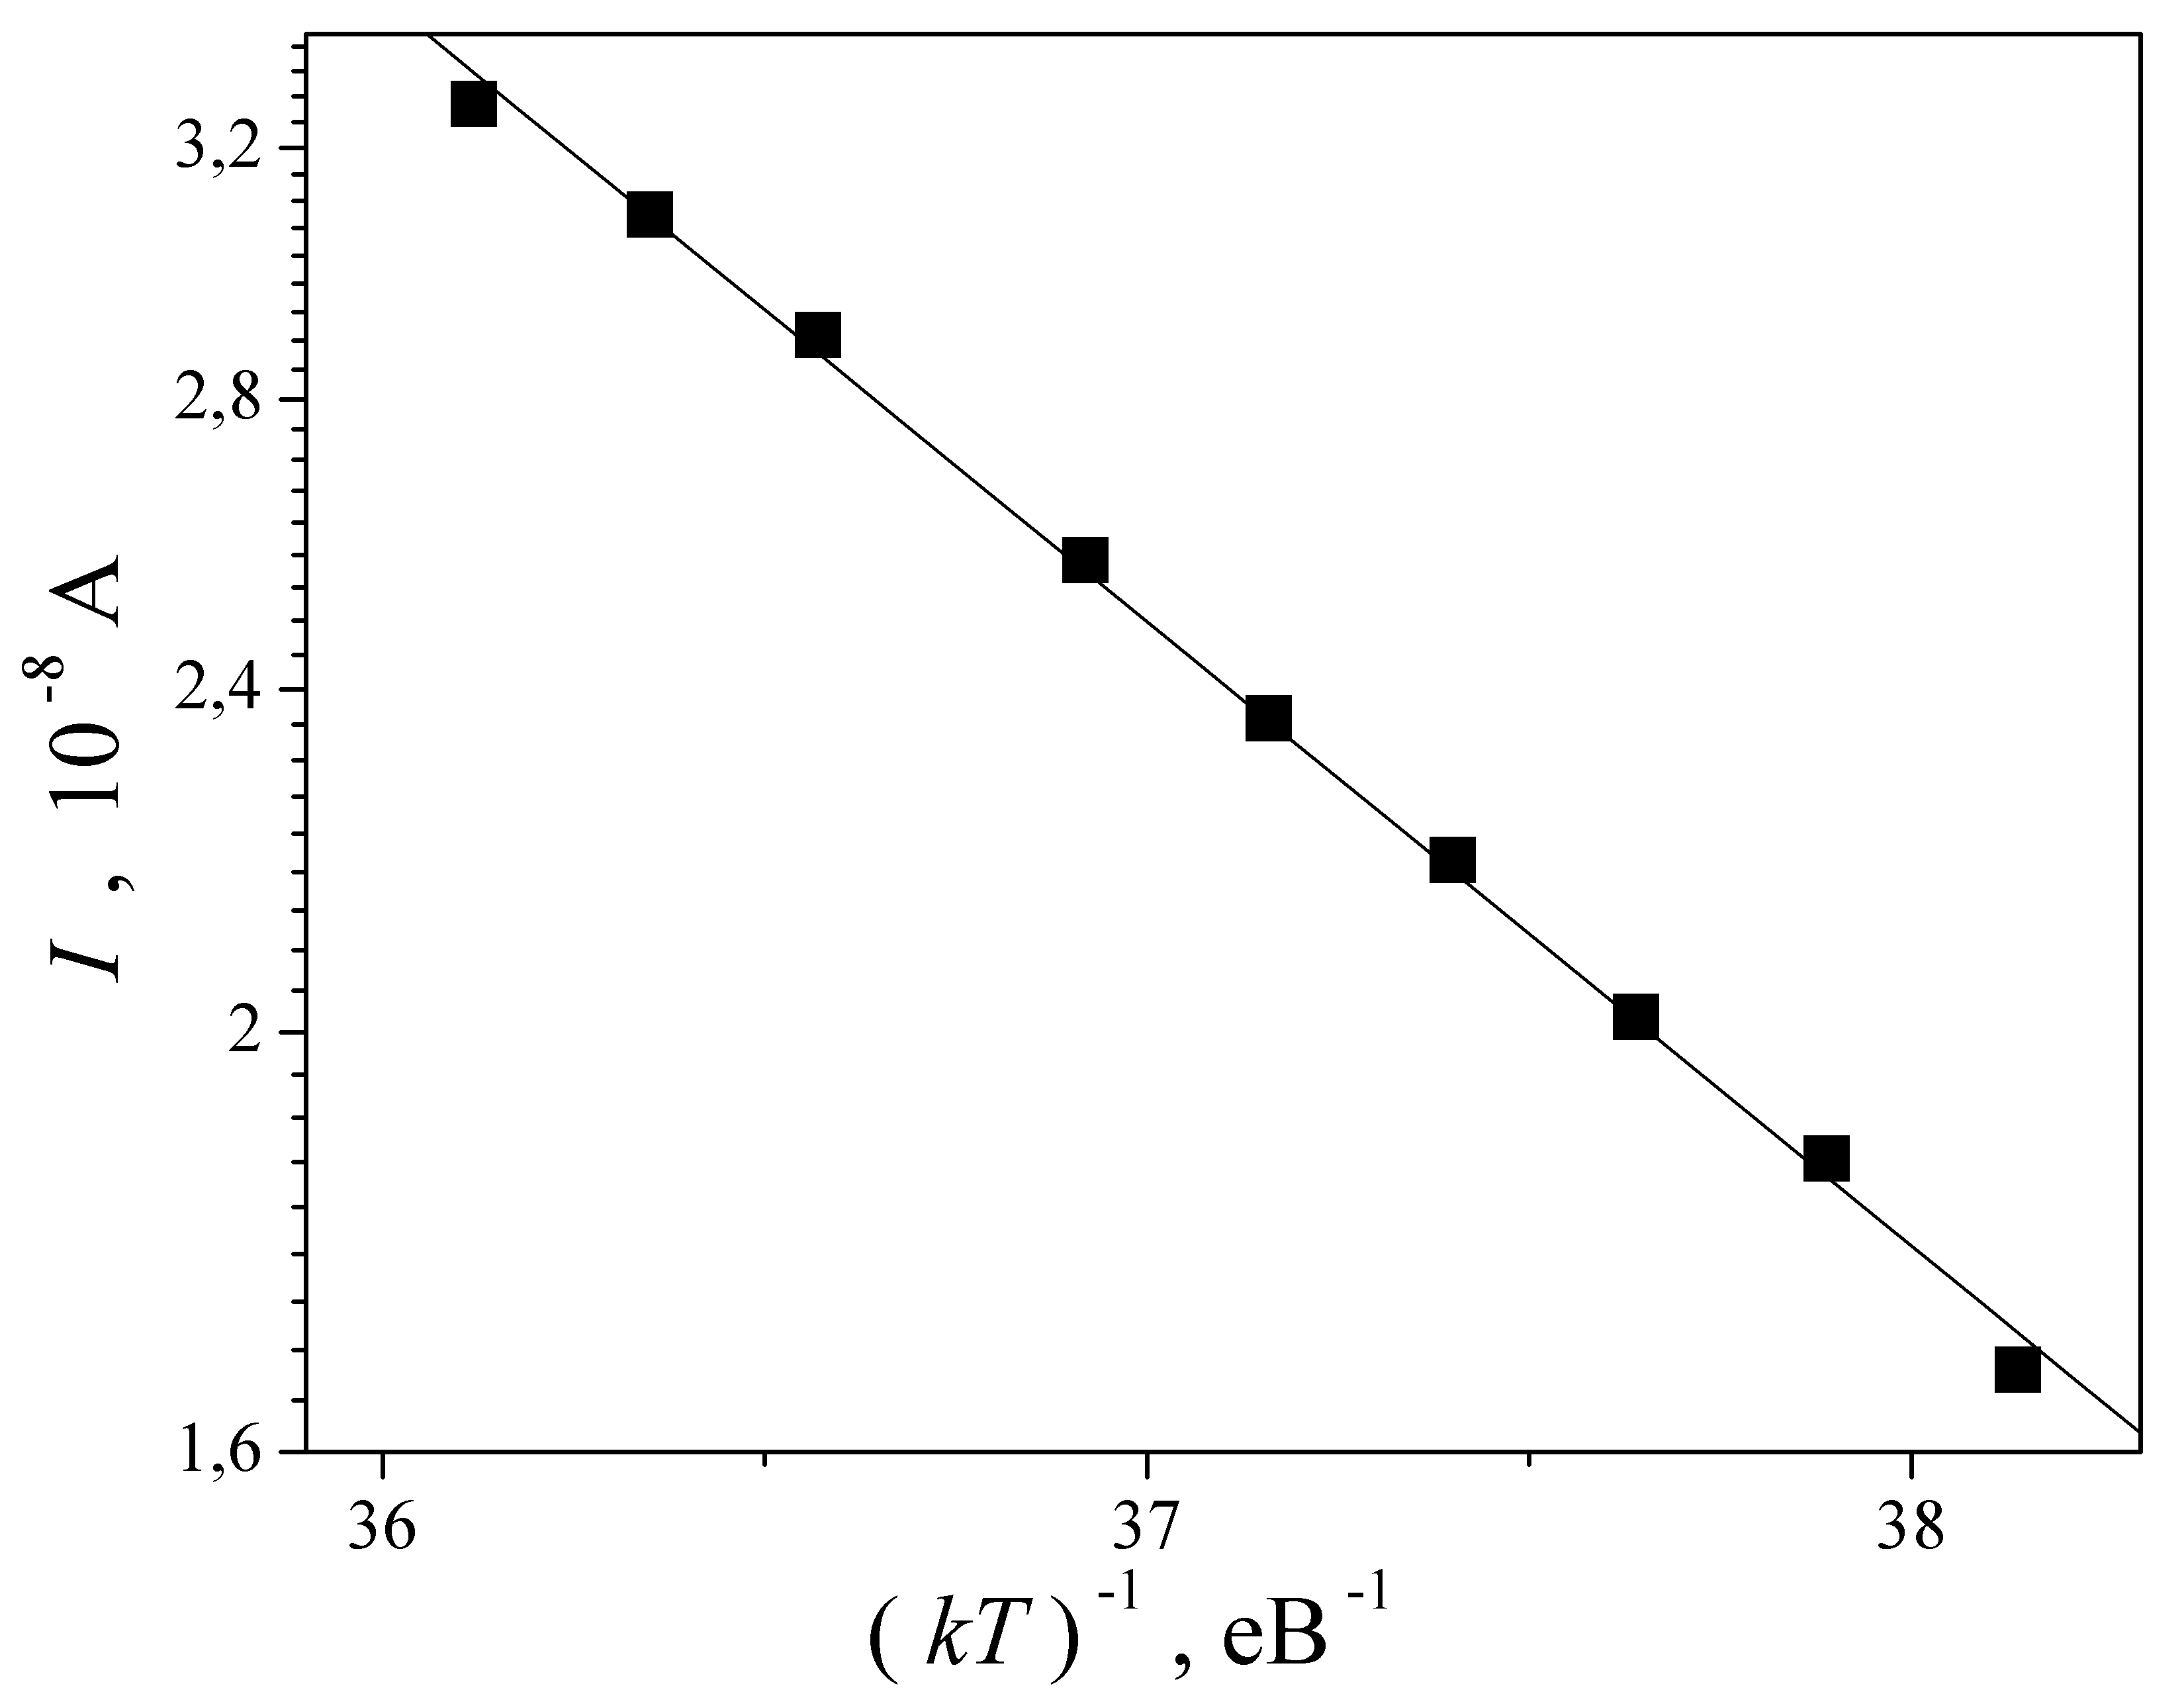
\includegraphics[width=0.65\textwidth]{figEa_MIS}%
\caption{\label{figEa_MIS}
Температурна залежність струму в SCLC--області  ($V=0,4$~В)
$\gamma$--опроміненої структури Si--SiO$_2$--Au до УЗО.
Точки --- експеримент,
пряма --- лінійна апроксимація.
}%
\end{figure}

Як відомо з літератури \cite{PersenkovBook}, при $\gamma$--опроміненні в системі Si--SiO$_2$
відбувається релаксація механічних напруг,
утворюються нові заряджені дефекти та заряджаються пастки, що вже були раніше.
Внаслідок цих процесів рельєф густини об'ємного заряду вирівнюється.
Вважається, що основними пастками, які захоплюють негативний заряд є центри інтерфейсній границі розділу,
тоді як позитивний заряд накопичується на $E'$--центрах, $E'_\delta$-- центрах та трьох рівнях, пов'язаних
з напруженими зв'язками \cite{SiO2:Devine,SiO2:Lenahan}.
Проте при фотонному дефектоутворенні (використанні рентгенівських променів чи $\gamma$--квантів) останні рівні утворюються у значно меншій кількості, ніж два перших \cite{SiO2:Devine}.
Зауважимо, що в нашому випадку достатньо низькі температура та парціальний тиск кисню призводили до утворення тонких шарів окису кремнію, проте в літературі \cite{SiO2:Cantin} показано, що в цьому випадку утворюються такі самі радіаційні дефекти, як і для прошарків більшої товщини.

Зазначимо, що ключовим фактором створення електричноактивних радіаційних дефектів у кремнієвих МОН структурах вважається вміст водню \cite{SiO2:Cantin}.
Плівки SiO$_2$ отримані термічним шляхом містять значну кількість атомів водню \cite{PersenkovBook}.
Утворення інтерфейсних рівнів пов'язується з розривом зв'язків $\equiv\!\text{Si}\!-\!\text{H}$ на границі Si--SiO$_2$ за наявності гарячих носіїв заряду \cite{SiO2:Mahapatra,SiO2:Esseni}.
Утворені ненасичені зв'язки $\equiv\text{Si}-$  діють як електронні пастки.
Загалом, розрізняють дефекти подібного типу залежно від орієнтації кремнієвої підкладки, на якій вирощено шар окису.
Вважається, що на границі з кремнієм, орієнтованим в площині (111), з'являються $P_b$--центри, тоді
як для (100) підкладки характерним є поява $P_{b1}$-- та $P_{b0}$--центрів \cite{SiO2:Rev}.
Ці центри хімічно ідентичні, проте характеризуються різною електричною активністю.
Крім того, при $\gamma$--опроміненні систем Si--SiO$_2$, вирощених на (111) підкладках, густина радіаційних поверхневих центрів вища ніж для (100) і досягає величини близько $10^{12}$~еВ/см при дозі $10^{7}$~рад \cite{PersenkovBook}.

Відомо що при перевищенні дози опромінення $\gamma$--квантами величини близько $5\cdot10^5$~рад у структурах Si--SiO$_2$ на основі кремнію з електронною провідністю спостерігається немонотонних розподіл інтерфейсних станів по енергії \cite{PersenkovBook},
причому, згідно з даними роботи \cite{ParchSiO2}, найбільша густина поверхневих станів спостерігається при
$E_c-(0,32\pm0,04)$~еВ.
Це величина збігається з отриманим значенням $E_x$.
Це свідчить про те, що проходження струму при малих прямих зміщеннях в досліджених структурах після опромінення пов'язане саме із захопленням електронів $P_b$--центрами.
Накопичення від'ємного заряду на інтерфейсі також викликає збільшення висоти бар'єру,
що відображається у виявленому зменшенні ТЕ струму.
В літературі і раніше повідомлялося про зменшення струмів внаслідок опромінення МОН--структур \cite{SiO2:Niu}.
Проте, як вже зазначалося вище, основною причиною зменшення ТЕ компоненти струму є дефектоутворення у приповерхневому шарі кремнію та відповідне зростання $n_\mathrm{id}$.

В результаті УЗО, як видно з Рис.~\ref{figIV_MIS}, спостерігається збільшення струму, обмеженого просторовим зарядом.
Зокрема, при $t_\mathtt{UST}=60$~хв, цей струм перевищив термоемісійний в дослідженому діапазоні напруг.
Параметри, отримані шляхом апроксимацій ВАХ, зведені в Таблиці~\ref{tabMIS}.
Виявлене збільшення $I_0$ свідчить, відповідно до формули~(\ref{eqIoSCLC}), про АІ зменшення концентрації $P_b$--центрів, а зростання $m_\mathrm{F}$ (або, що те саме, $T_c$) --- про звуження енергетичного розподілу відповідних рівнів.
З літератури \cite{SiO2:Takakura,SiO2:Wurzer} відомо, що відпал $P_b$--центрів відбувається внаслідок пасивації ненасичених зв'язків атомами водню.
Тобто, отримані результати свідчать, що УЗО стимулює дифузію водню.
Загалом, подібні процеси спостерігалися і раніше \cite{Ostap:SiO2,Ostap:PhotoLum,ostapenko1997}, проте в нашому випадку мова йде про АІ відпал радіаційних дефектів.


Як відомо \cite{Jafar}, випадок $m_\mathrm{F}=2$ відповідає наявності пасток з однаковим енергетичним рівнем.
Виявлене звуження енергетичного розподілу свідчить про певну вибірковість АІ процесів пасивації:
внаслідок УЗО атоми Н осідають переважно на зв'язки, яким відповідає цілком певне розташування рівнів у забороненій зоні.
На погляд автора, визначальним фактором того, які саме зв'язки будуть заповнені під час АІ відпалу є механічні напруги, неоднорідним чином розподілені на інтерфейсі.
Відомо, що дифузійна здатність домішок у напівпровідникових кристалах залежить від механічних напруг \cite{AZIZ2001}.
До речі, це може бути основною причиною переміщення водню в ультразвуковому полі.
Проте в даному випадку хотілося б звернути увагу в першу чергу на те, що від рівня деформації залежить ефективність АІ пасивації, а отже УЗО сприяє підвищенню однорідності структури.

Наслідком часткового зменшення від'ємного заряду, накопиченого $P_b$--центрами на інтерфейсі, є часткове зменшення висоти бар'єру, що викликає зростання ТЕ струму --- див. дані для $I_s$ в Таблиці~\ref{tabMIS}.
Водночас виявлене зменшення послідовного опору свідчить про АІ частковий відпал радіаційних дефектів у об'ємі напівпровідника.

Звільнені під час утворення $P_b$--центрів при $\gamma$--опроміненні атоми водню можуть
а)~взаємодіяти з іншими атомами Н на границі розділу, ще зв'язаними, відривати їх та викликати утворення додаткових $P_b$--центрів \cite{SiO2:Devine};
б)~переміщуючись в кремнієву підкладку генерувати дефекти та викликати деактивацію легуючої домішки \cite{SiO2:DiMaria};
б)~рухатися в об'єм діелектрика, де, за наявності гарячих носіїв заряду, призводити до появи $E'$--центрів (так званих, об'ємних пасток, bulk--oxide trap) внаслідок розриву зв'язків в системі $\equiv\!\text{Si}\!-\!\text{O}$ \cite{SiO2:Mahapatra,SiO2:Esseni}.
Тобто, за своєю структурою $E'$--центри --- це вакансії кисню в SiO$_2$ \cite{SiO2:Takakura,SiO2:Devine},
які накопичують позитивний заряд.
Загальна концентрація цих дефектів при $\gamma$--опроміненні з дозою $10^{7}$~рад складає приблизно $10^{18}$~см$^{-3}$, проте по товщині оксидної плівки вони розподілені нерівномірно, найбільша кількість спостерігається біля границі з кремнієм \cite{PersenkovBook}.
Ці центри стабільні при кімнатній температурі \cite{SiO2:Mahapatra}, температура відпалу складає $(200\div400)^\circ$C.

Наявність розірваних зв'язків в об'ємі оксиду є причиною появи так званих напругоіндукованих струмів втрат (stress-induced leakage current, SILC) \cite{SiO2:Mahapatra,SiO2:DiMaria}.
На нашу думку, саме цей струм і реєструється в опромінених структурах при зворотному зміщенні (див.~Рис.~\ref{figIV_MIS},а та б).
Відомо \cite{SiO2:Esseni,SiO2:DiMaria}, що перенесення заряду для SILC пов'язане з тунелювання по пасткам (trap--assisted tunneling, ТАТ) .
Відповідно до \cite{TAT:Gilmore,TAT:GopalSST,TAT:Gopal}, польова залежність ТАТ--струму може бути записана у наступному вигляді:
\begin{equation}\label{eqIVTAT}
  I=I_{0,\mathrm{TAT}}\,(U_d+V_R)\exp\left(-\frac{R_\mathrm{TAT}}{F_m}\right),
\end{equation}
де
$I_{0,\mathrm{TAT}}$ та $R_\mathrm{TAT}$ не залежать від напруги,
$I_{0,\mathrm{TAT}}$ прямопропорційно залежить від концентрації пасток,
$U_d$ --- висота бар'єру.
На Рис.~\ref{figIV_MIS} наведено результати апроксимації експериментально отриманих зворотних гілок ВАХ згідно з формулою~(\ref{eqIVTAT}), що підтверджують висловлене припущення про природу цього струму.
Відхилення від очікуваною залежності при великих зміщеннях може бути пов'язане з впливом послідовного опору.
Величини визначених в результаті апроксимації параметрів (див.~Таблицю~\ref{tabMIS}) свідчать про АІ відпал радіаційно утворених пасток та зниження висоти бар'єру.
На нашу думку, відпал $E'$--центрів також пов'язаний з викликаною УЗО дифузією міжвузольних атомів, у даному випадку  кисню.

Збільшення прямого струму та зменшення зворотного в результаті УЗО викликає збільшення коефіцієнта випрямлення струму
$K_\mathrm{RECT}$, який суттєво зменшився в результаті $\gamma$--опромінення.
Так в Таблиці~\ref{tabMIS} наведено значення цієї величини при напрузі 0,5 В.
Це також свідчить, що УЗО при температурах, близьких до кімнатних, здатна частково відновлювати характеристики напівпровідникових пристроїв, деградованих внаслідок дії радіаційного опромінення.







\section*{Висновки до розділу \ref{Ch_UST_MW}}
\addcontentsline{toc}{section}{Висновки до розділу \ref{Ch_UST_MW}}
  \begin{enumerate}
\item Експериментально досліджено вплив мікрохвильового опромінення на параметри точкових дефектів (поперечний переріз захоплення електронів,
розташування енергетичних рівнів у забороненій зоні) в монокристалах $n$--6$H$--SiC, $n$--GaAs та епітаксійних структурах на основі арсеніду галію.


\item Показано, що  дефекти у приповерхневому шарі, які ефективно захоплюють носії заряду, є власними вакансійного типу.
Виявлені зміни параметрів пасток обумовлені індукованим мікрохвильовим випромінюванням
збільшенням кількості міжвузольних атомів та релаксацією внутрішніх механічних напруг.
Показано, що наявність стискуючих напруг у приповерхневому шарі сприяє перетворенню дефектних комплексів внаслідок високочастотного опромінення.

     \item Вперше експериментально досліджено вплив ультразвукової обробки на параметри структури Au--TiB$_x$--$n$--$n^+$--GaAs з контактом Шотки
 в залежності від частоти та інтенсивності.
Виявлено, що вплив ультразвуку на зворотні гілки ВАХ значно суттєвіший ніж на прямі.
 Експериментально встановлено, що при малій інтенсивності ультразвуку (менше 2,5~Вт/см$^2$) характер УЗ впливу за величину зворотного струму залежить від механізму перенесення заряду:
  якщо домінуючим механізмом є тунельний, то УЗО викликає збільшення зворотного струму, якщо термоемісійний --- зменшення.
  Показано, що причиною виявлених ефектів може бути акусто--стимульована дифузія точкових дефектів.
  Зростання зворотного струму при перевищенні порогового значення інтенсивністю УЗО пов'язане з акусто--індукованою генерацією дефектів.

\item Виявлено, що зі збільшенням частоти ультразвукової обробки інтенсифікуються процеси перебудови дефектів.

\item Показано, що ультразвукова обробка здатна викликати зменшення розкиду параметрів і підвищення однорідності характеристик, створених в єдиному технологічному процесі.

\item Досліджено вплив ультразвукової обробки на парметри структур метал--окис--напівпровідник.
   Виявлено можливість низькотемпературного відпалу радіаційних дефектів в системі Si--SiO$_2$.
   Показано, що акустоіндукований відпал пов'язаний з дифузією міжвузольних атомів.

\item Виявлено, що ультразвукова обробка сприяє звуженню енергетичного спектру радіаційноіндукованих пасток
на інтерфейсі системи    Si--SiO$_2$.


\end{enumerate}	



Основні результати даного розділу представлені в роботах \cite{Olikh:SPQEO2003,Olikh:PJE2004,Olikh:PhChOM2005,Olikh:PZTF2006,Gorb2010,
3Tomsk,50IUFFC,9APTTE,ICU2007GA,6DrogGorb}.



%\cite{PersenkovBook}
%При гамма--опроміненні релаксація механічних напруг в системі Si--SiO$_2$:
%частина дірок, що утворилася при іонізації захоплюється на рівні напружених зв'язків, що призводить до їх розриву
%термічно отримані плівки SiO$_2$ поліморфні,
%%містять велику кількість водню
%
%%Е' центри (пастки дірок) розподілені нерівномірно, найбільша концентрація біля границі з Si.
%%загальна концентрація при 1е7 рад ---  близько 1е18 см-3.
%
%тривалентний кремній --- донороподібний центр,
%відповідає за додатній заряд, який накопичується в об'ємі при опроміненні
%
%%при опроміненні Si--SiO$_2$ утворюються нові заряджені дефекти та заряджаються пастки,
%%що вже були,
%%рельєф густини об'ємного заряду вирівнюється
%
%швидкі поверхневі стани розташовані в приповерхневому шарі напівпровідника,
%повільні --- в приграничній області оксиду.
%
%%густина утворених поверхневих станів при гамма--опроміненні найбільша при (111), найменша (100),
%%при 1е7 рад порядку 1е12 еВ/см2
%
%кореляція між густиною швидких поверхневих станів Nss та пасткових центрів в об'ємі SiO$_2$ No
%Nss=3.75t-6 см/еВ No,
%а отже однакова причина утворення дефектів:наявність напружених валентних зв'язків між атомами та їх розрив в результаті іонізації.
%
%%при опроміненні гамма--квантами найбільша густина станів в околі Ес-(0,3-0,4)еВ (для електронного, для діркового не так),
%%причому така нерівномірність спостерігається лише при перевищенні дозою порогу близько 5е5 рад.
%
%швидкість поверхневої рекомбінації визначається густиною поверхневих станів
%s~Nss
%
%в об'ємі напівпровідника час життя змінюється мало при гамма-опроміненні, в приповерхневому шарі зменшується
%
%%\cite{ParchSiO2}
%%часткова компенсація напівпровідникової підкладинки в процесі радіаційного дефектоутворення
%%гамма--кванти, до 2е7 рад, максимум спектру поверхневих станів Ес-(0,32+-0,04) ев, що характерно для високих доз -- див попередню
%%
%%електронне опромінення (n-тип, (100)) --- максимум густини поверхневих станів Ес-0,3 еВ \cite{LaiSiO2}
%
%
%
%%Interface trap (Nit) утворюються внаслідок розриву зв'язків $\equiv\!\text{Si}\!-\!\text{H}$ на інтерфейсі Si--SiO$_2$,
%%в результаті утворюються $\equiv\text{Si}-N_\text{iT}$, які реєструються як Pb центри.
%%Звільнені атоми водню рухаються в об'єм діелектрика.
%%За наявності гарячих носіїв заряду при цьому генеруються bulk--oxide trap Not внаслідок розриву $\equiv\!\text{Si}\!-\!\text{O}$.
%%Розірвані зв'язки $\equiv\!\text{Si}\!-\!\text{O}$ в об'ємі оксиду викликають появу stress-induced leakage current (SILC).
%%However, unlike $\equiv\!\text{Si}\!-\!\text{H}$  bonds, broken $\equiv\!\text{Si}\!-\!\text{O}$ bonds are not known to recover
%%at room temperature after the stress is removed.
%%В роботі пропонується, що $\equiv\!\text{Si}\!-\!\text{H}$ bonds are broken by holes (and not by electrons). \cite{SiO2:Mahapatra}
%
%
%%Гарячі електрони ведуть до звільнення водню з інтерфейсу Si--SiO$_2$,
%%міграція Н в оксиді викликає появу bulk--oxide trap.
%%Механізм SILC --- trap--assisted tunneling
%%The results reported so far demonstrate that in the channel hot electron stress conditions there is no correlation between and SILC generation.
%%В самій роботі Nit generation is evidently related to stress-induced leakage current (H/D) release \cite{SiO2:Esseni}
%%
%%SILCs  (This  phenomenon  is  often  referred  to  as  trap-assisted  tunneling ) can  be  best  explained  by  the generation  of  neutral  electron  traps  in  the  oxide  layer.
%%These  studies  have  directly  shown  the  relationship  of SILCs  to  the  trap  creation  phenomenon.
%%Trapped  holes  or  sites  produced by  trapped-hole  annihilation  by  free  electrons  will  be demonstrated  not  to  contribute  to  SILC  for  most  stressing conditions.
%%Since  the  oxide  deterioration  producing  SILC  will  be shown  here  to  be  caused  by  electron  heating  in  the  oxide layer,
%%oxide  defect  formation  due  to  hot  carriers  will  be briefly  reviewed.
%%The  production  of  interface  states or  traps by  the  annihilation  of  trapped  holes  and/or  their  presence  is
%%one  component  of  the  oxide  degradation  process.
%%The other  component  is  due  to  the  trap  creation  process  also  caused by  hot  electrons.
%%  Also, the  most  significant  component  contributing  to  the  SILC  in the  experiments  discussed here  appears to  be due  to  the  generation  of  the  neutral-electron  traps,  not  the  interface  states and/or  anode positive  charge.
%%Also,  generation--recombination  sites  and boron  deactivation  can be produced  in  the Si  substrate by  the hydrogen.
%%However,  during  trap  creation,  many  different  defect  sites  with  different  processing  dependencies  from  one wafer  run  to  another  can  occur.  These  defects  include  interface  states, generation-recombination  centers  in  the  Si  substrate,  neutral  electron  traps  in  the  oxide  bulk  distributed  away  from  the  cathode/oxide  interface,  and positively  charged  oxide  sites  (mostly  <<slow  states>> )  near the  anode/oxide  interface.\cite{SiO2:DiMaria}
%
%%На границі з (111) --- Pb центр,
%%на границі з (100) --- Pb1 та Pb0.
%%центри хімічно ідентичні, різна електрична активність (Pb1, здається не активний)
%%взагалі робота --- огляд.. там багато всякого про інтерфейсні рівні \cite{SiO2:Rev}
%
%%Опромінення гамма--квантами, доза 1е6,
%%утворилися нові інтерфейсні рівні (порядку 3е10 см-2).. головна ідея -- при прикладенні напруги в опромінених структурах генеруються більше пасток \cite{AASSIME1997}
%
%%тонкі (20--40 ангстрем) шари , опромінення х-променями (10 кев), утворюються такі самі дефекти (Е' (позитивно заряджені вакансії кисню) та два типи Pb, бо (100) пластинки)
%%that one key parameter for the moddication of the electrically  active  defects  in  MOS  structures  is their hydrogen content \cite{SiO2:Cantin}
%
%%опромінення протонами (еквівалентна доза гамма--квантів близько 1е6) --- зміни струмів різних (там транзистор) можуть бути і від'ємні після опроміненя
%%is  shown  to be  a result  of  the increase  in  fixed oxide  charge  and  surface  trap  densities,  in combination with the different SRH  recombination rate limiting
%%mechanisms in the presence of high density surface traps \cite{SiO2:Niu}
%
%%огляд радіаційних дефектів в SiO2:
%%пастки, які захоплюють позитивний заряд--- відпалюються при температурах 200--400 градусів цельсію
%%Е' центр (вакансія кисню) --- основний,
%%$E'_\delta$ (комплекс вакансія кисню--кремній), тяжко утворюється при дії фотонів (гамма та Х)
%%три пастки пов'язані з напруженими зв'язками
%%негативний заряд
%%Pb центри (причому звільнені атоми водню можуть взаємодіяти і іншими, ще зв'язаними, і відривати їх також)
%%як не дивно, знову вакансії кисню
%%we generally expect the neutral oxygen-vacancy to be a hole trap, it may also trap electrons leading  to a negatively charged state in the SiO2  bandgap
%%about 1  eV below the conduction band edge \cite{SiO2:Devine}
%
%%decrease of base current during annealing. We  found that two mechanisms
%%are responsible for annealing: the recombination  of charges and
%%the bonding of hydrogen atoms on interface traps.
%%процеси з двома енергіями активації -- 0,23 ев та 0,046ев
%%As  the  Shockley-Read-Hall  current  is  proportional to the
%%density of  interface traps,  the decrease of  the base current
%%is proportional to  the  density of  the  annealed interface traps. \cite{SiO2:Wurzer}
%
%%Ще одна робота про результат опромінення: переважно Е', Pb (або два варіанти для 100) все повторюється..
%%і те, що Pb амфотерний (може захоплювати і дірки, якщо його рівень в нижній половині забороненої зони)\cite{SiO2:Lenahan}
%
%%It is well established nowadays that one of the main hole trapping centres responsible for irradiation-induced positive
%%charge is the E'-centre. Electron spin resonance (ESR)
%%studies have revealed that the E'-centre is a defect resulting
%%from an oxygen vacancy in SiO2. A direct correlation has been
%%established between the annealing of the oxide-trapped charge.
%%The key SiO2/Si interface defect is called Pb-centre and
%%corresponds to a silicon dangling bond at the interface, back-
%%bonded by three other silicon atoms . Passivation of these dangling bonds (DBs) occurs
%%through binding with hydrogen.
%%From this result it is concluded that the degradation
%%and recovery of the device performance are mainly caused by
%%trapped-oxide charge
%%Вираз для струму, пов'язаного з поверхневою рекомбінацією, близький до того, що використовували ми
%%\cite{SiO2:Takakura}
%
%%залежність дифузійної здатності від механічних напруг \cite{AZIZ2001}
%%
%%\cite{Ostap:SiO2} стан границі Si--SiO2, підсилення дифузії водню
%%\cite{Ostap:PhotoLum,ostapenko1997} підсилення дифузії водню
